%\documentclass[mat2, tisk]{fmfdelo}
% \documentclass[fin2, tisk]{fmfdelo}
\documentclass[isrm2, tisk]{fmfdelo}


\usepackage[caption = false]{subfig}


% - ime datoteke z viri (vključno s končnico .bib), če uporabljate BibTeX


% \documentclass[ped, tisk]{fmfdelo}
% Če pobrišete možnost tisk, bodo povezave obarvane,
% na začetku pa ne bo praznih strani po naslovu, …

%%%%%%%%%%%%%%%%%%%%%%%%%%%%%%%%%%%%%%%%%%%%%%%%%%%%%%%%%%%%%%%%%%%%%%%%%%%%%%%
% METAPODATKI
%%%%%%%%%%%%%%%%%%%%%%%%%%%%%%%%%%%%%%%%%%%%%%%%%%%%%%%%%%%%%%%%%%%%%%%%%%%%%%%

% - vaše ime
\avtor{Kevin Štampar}

% - naslov dela v slovenščini
\naslov{Orodje za grafični prikaz lastnosti Bézierjevih in PH krivulj}

% - naslov dela v angleščini
\title{Tool for graphically displaying the properties of Bézier and PH curves}

% - ime mentorja/mentorice s polnim nazivom:
%   - doc.~dr.~Ime Priimek
%   - izr.~prof.~dr.~Ime Priimek
%   - prof.~dr.~Ime Priimek
%   za druge variante uporabite ustrezne ukaze
\mentor{prof.~dr.~Emil Žagar}
% \somentor{...}
% \mentorica{...}
% \somentorica{...}
% \mentorja{...}{...}
% \somentorja{...}{...}
% \mentorici{...}{...}
% \somentorici{...}{...}

% - leto magisterija
\letnica{2024}

% - povzetek v slovenščini
%   V povzetku na kratko opišite vsebinske rezultate dela. Sem ne sodi razlaga
%   organizacije dela, torej v katerem razdelku je kaj, pač pa le opis vsebine.
\povzetek{Tukaj napišemo povzetek vsebine. Sem sodi razlaga vsebine in ne opis tega, kako je delo organizirano.}

% - povzetek v angleščini
\abstract{An abstract of the work is written here. This includes a short description of
the content and not the structure of your work.}

% - klasifikacijske oznake, ločene z vejicami
%   Oznake, ki opisujejo področje dela, so dostopne na strani https://www.ams.org/msc/
\klasifikacija{74B05, 65N99}

% - ključne besede, ki nastopajo v delu, ločene s \sep
\kljucnebesede{integracija\sep kompleks}

% - angleški prevod ključnih besed
\keywords{integration\sep complex} % angleški prevod ključnih besed

% - neobvezna zahvala
\zahvala{
    Zahvaljujem se mentorju za zelo sproščen odnos!
}

% - program dela, ki ga napiše mentor z osnovno literaturo
\programdela{
    Mentor naj napiše program dela skupaj z osnovno literaturo.
}

\osnovnaliteratura{
% Literatura mora biti tukaj posebej samostojno navedena (po pomembnosti) in ne
% le citirana. V tem razdelku literature ne oštevilčimo po svoje, ampak uporabljamo
% ukaz \vnosliterature, v katerega vpišemo citat
%    \vnosliterature{24ac2b10-13c2-3e17-bc91-5f7366bf076c}
}

% - ime datoteke z viri (vključno s končnico .bib), če uporabljate BibTeX
\literatura{literatura.bib}

%%%%%%%%%%%%%%%%%%%%%%%%%%%%%%%%%%%%%%%%%%%%%%%%%%%%%%%%%%%%%%%%%%%%%%%%%%%%%%%
% DODATNE DEFINICIJE
%%%%%%%%%%%%%%%%%%%%%%%%%%%%%%%%%%%%%%%%%%%%%%%%%%%%%%%%%%%%%%%%%%%%%%%%%%%%%%%

% naložite dodatne pakete, ki jih potrebujete
\usepackage{units}        % fizikalne enote kot \unit[12]{kg} s polovico nedeljivega presledka, glej primer v kodi
\usepackage{graphicx}     % za slike
% \usepackage{tikz}
% VEČ ZANIMIVIH PAKETOV
% \usepackage{array}      % več možnosti za tabele
% \usepackage[list=true,listformat=simple]{subcaption}  % več kot ena slika na figure, omogoči slika 1a, slika 1b
% \usepackage[all]{xy}    % diagrami
% \usepackage{doi}        % za clickable DOI entrye v bibliografiji
\usepackage{enumitem}     % več možnosti za sezname

% Za barvanje source kode
% \usepackage{minted}
% \renewcommand\listingscaption{Program}

% Za pisanje psevdokode
\usepackage{algpseudocode}  % za psevdokodo
\usepackage{algorithm}
\usepackage{algorithmicx}
\usepackage{mathtools}
\usepackage{hyperref}
\usepackage{graphics}
\floatname{algorithm}{Algoritem}
\renewcommand{\listalgorithmname}{Kazalo algoritmov}

% deklarirajte vse matematične operatorje, da jih bo LaTeX pravilno stavil
% \DeclareMathOperator{\...}{...}

% vstavite svoje definicije ...
\newcommand{\R}{\mathbb R}
\newcommand{\N}{\mathbb N}
\newcommand{\Z}{\mathbb Z}
% Lahko se zgodi, da je ukaz \C definiral že paket hyperref,
% zato dobite napako: Command \C already defined.
% V tem primeru namesto ukaza \newcommand uporabite \renewcommand
\newcommand{\C}{\mathbb C}
\newcommand{\Q}{\mathbb Q}
\newcommand{\Pn}{\mathbb P_n}
\newcommand{\p}{\mathbf{p}}
\newcommand{\B}{\mathbf{B}}

\newcommand{\groupimagewidth}{0.28\textwidth}
%0.27 = 33 strani

%Bernstein
\newcommand{\bernsteinbase}[3]{\binom{#1}{#2}t^{#1}(1-t)^{#2}}
\newcommand{\bernstein}[2]{\binom{#1}{#2}t^{#2}(1-t)^{#1-#2}}
\newcommand{\lilb}[2]{B_{#1}^{#2}(t)}
\newcommand{\bigb}[1]{B_{#1}(t)}
\newcommand{\bigbb}[1]{\textbf{B}_{#1}(t)}
\newcommand{\bigbbod}[2]{\textbf{B}_{#1}(#2)}
\newcommand{\bigbbt}{\textbf{B}(t)}
\newcommand{\bigbo}[1]{B'_{#1}(t)}
\newcommand{\bernsteinsum}[2]{\sum_{#1=0}^{#2} \beta_{#1}\lilb{#1}{#2}}
\newcommand{\bernsteinsump}[2]{\sum_{#1=0}^{#2} \p_{#1}\lilb{#1}{#2}}
\newcommand{\bernsteinsumtri}[3]{\sum_{#1=0}^{#2} #3_{#1}\lilb{#1}{#2}}
\newcommand{\bernsteinsumtritri}[3]{\sum_{#1=0}^{#2} #3\lilb{#1}{#2}}
\newcommand{\bernsteinsumtridva}[2]{\sum_{#1=0}^{#2} \lilb{#1}{#2}}

\newcommand{\bsum}{\bernsteinsum{i}{n}}

% Komentarji znotraj vsebine
\newcommand{\mycomment}[1]{\textbf{\textcolor{red}{#1}}}
\newcommand{\missingref}[1]{\mycomment{referenca-#1}}


%%%%%%%%%%%%%%%%%%%%%%%%%%%%%%%%%%%%%%%%%%%%%%%%%%%%%%%%%%%%%%%%%%%%%%%%%%%%%%%
% ZAČETEK VSEBINE
%%%%%%%%%%%%%%%%%%%%%%%%%%%%%%%%%%%%%%%%%%%%%%%%%%%%%%%%%%%%%%%%%%%%%%%%%%%%%%%

\begin{document}

    \section{Uvod}
    Napišite kratek zgodovinski in matematični uvod. Pojasnite motivacijo za problem, kje
    nastopa, kje vse je bil obravnavan. Na koncu opišite tudi organizacijo dela -- kaj je v
    katerem razdelku.


    \mycomment{Ker je v okviru magistrskega dela nastalo orodje za grafični prikaz konceptov, bo delo polno s slikovnimi primeri.}

    \newpage


    \section{Bézierjeve krivulje}\label{sec:bezierjeve-krivulje}

    \subsection{Bernsteinovi bazni polinomi}\label{subsec:bernsteinovi-polinomi}
    V tem podrazdelku bomo predstavili Bernsteinove bazne polinome in nekaj njihovih lastnosti, ki bodo ključne pri vpeljavi Bézierjevih krivulj.
    Začnimo z njihovo definicijo.
    \begin{definicija}
        \label{def:bernstein}
        Za nenegativna cela števila $n$ je $i$-ti \textit{Bernsteinov bazni polinom} podan s predpisom \[B_i^n(t)\coloneqq\bernstein{n}{i},\quad i\in\Z.\]
    \end{definicija}
    % V definiciji Bernsteinovega polinoma smo uporabili le bazne polinome z indeksi $i=0,\ldots,n$.
    \noindent Iz definicije je očitno, da so za indekse $i>n$, oziroma $i<0$, Bernsteinovi bazni polinomi ničelni.
    Pri določeni stopnji $n$ je neničelnih Bernsteinovih baznih polinomov torej $n+1$.
    Brez dokaza povejmo, da so linearno neodvisni in zato tvorijo bazo prostora polinomov stopnje manjše ali enake $n$ ($\mathbb{P}_n$).
    Takšni bazi pravimo \textit{Bernsteinova baza}, polinomu, izraženemu v njej, pa pravimo \textit{Bernsteinov polinom}.
    \begin{primer}
        \label{primer:bernsteinovi}
        Za primer si bomo ogledali Bernsteinove bazne polinome stopenj $n=0,1,2,3$.
        Pri stopnji $0$ imamo konstantni polinom s funkcijskim predpisom $B_{0}^{0}(t) = 1$.
        Za stopnjo $1$ dobimo dva polinoma s funkcijskima predpisoma $B_{0}^{1}(t) = 1-t$ in $B_{1}^{1}(t) = t$.
        Funkcijski predpisi kvadratnih in kubičnih Bernsteinovih baznih polinomov pa so:
        \begin{align*}
            &B_{0}^{2}(t) = (1-t)^2,\quad B_{1}^{2}(t) = 2t(1-t),\quad B_{2}^{2}(t) = t^2,  \\
            &B_{0}^{3}(t) = (1-t)^3,\quad B_{1}^{3}(t) = 3t(1-t)^2,\quad B_{2}^{2}(t) = 3t^2(1-t),\quad B_{3}^{3}(t) = t^3.
        \end{align*}
        Grafe polinomov iz primera si lahko ogledamo na sliki~\ref{fig:bernstein-base}.
    \end{primer}
    \begin{figure}[h!]
        \captionsetup[subfigure]{labelformat=empty}
        \centering
        \subfloat[$n=0$]{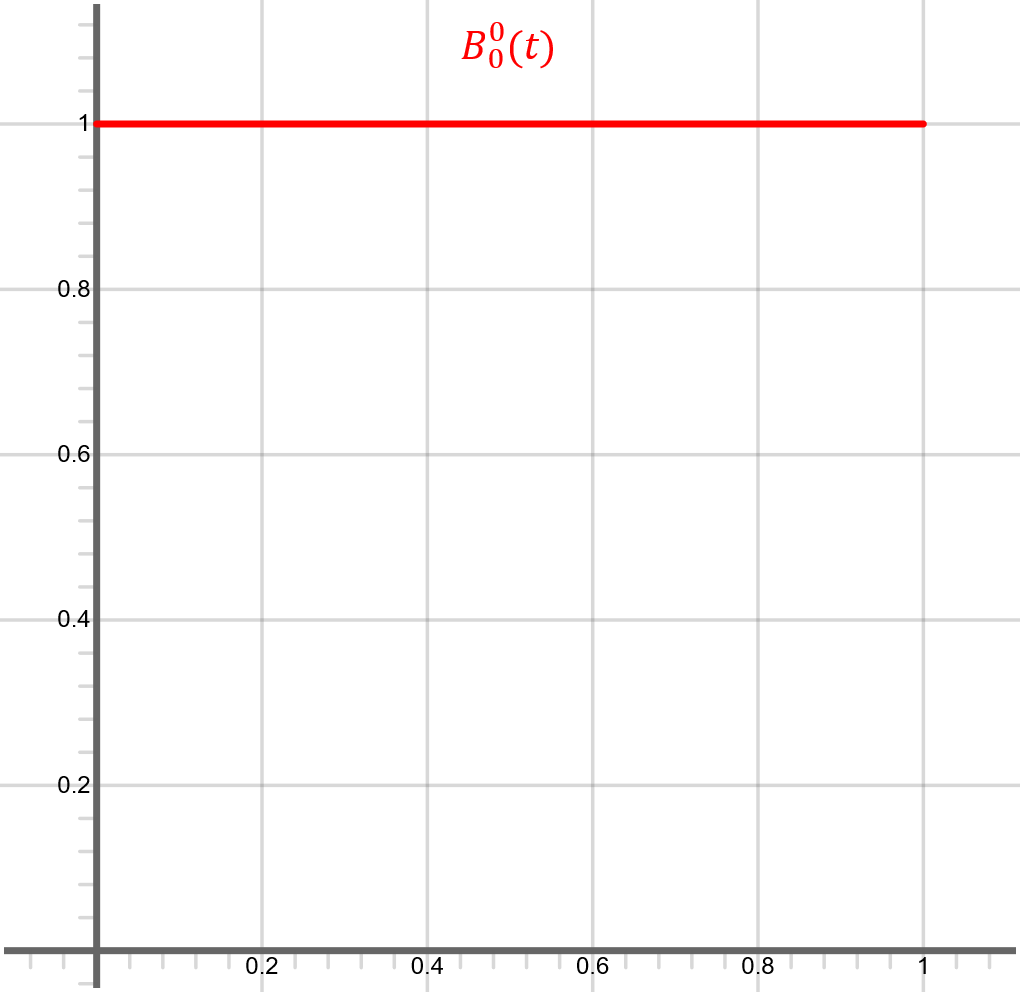
\includegraphics[width = \groupimagewidth]{images/bernstein-0}}
        \qquad
        \subfloat[$n=1$]{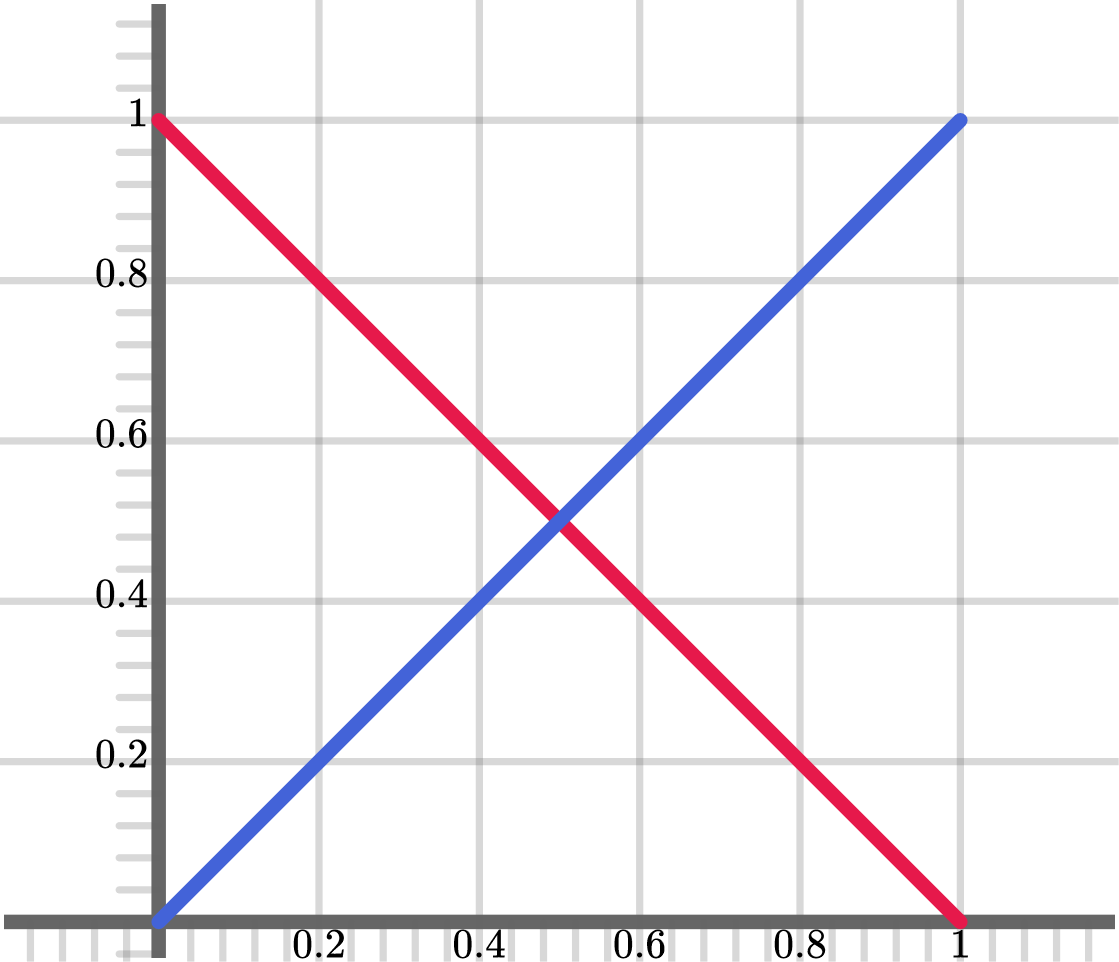
\includegraphics[width = \groupimagewidth]{images/bernstein-1}} \\
        \subfloat[$n=2$]{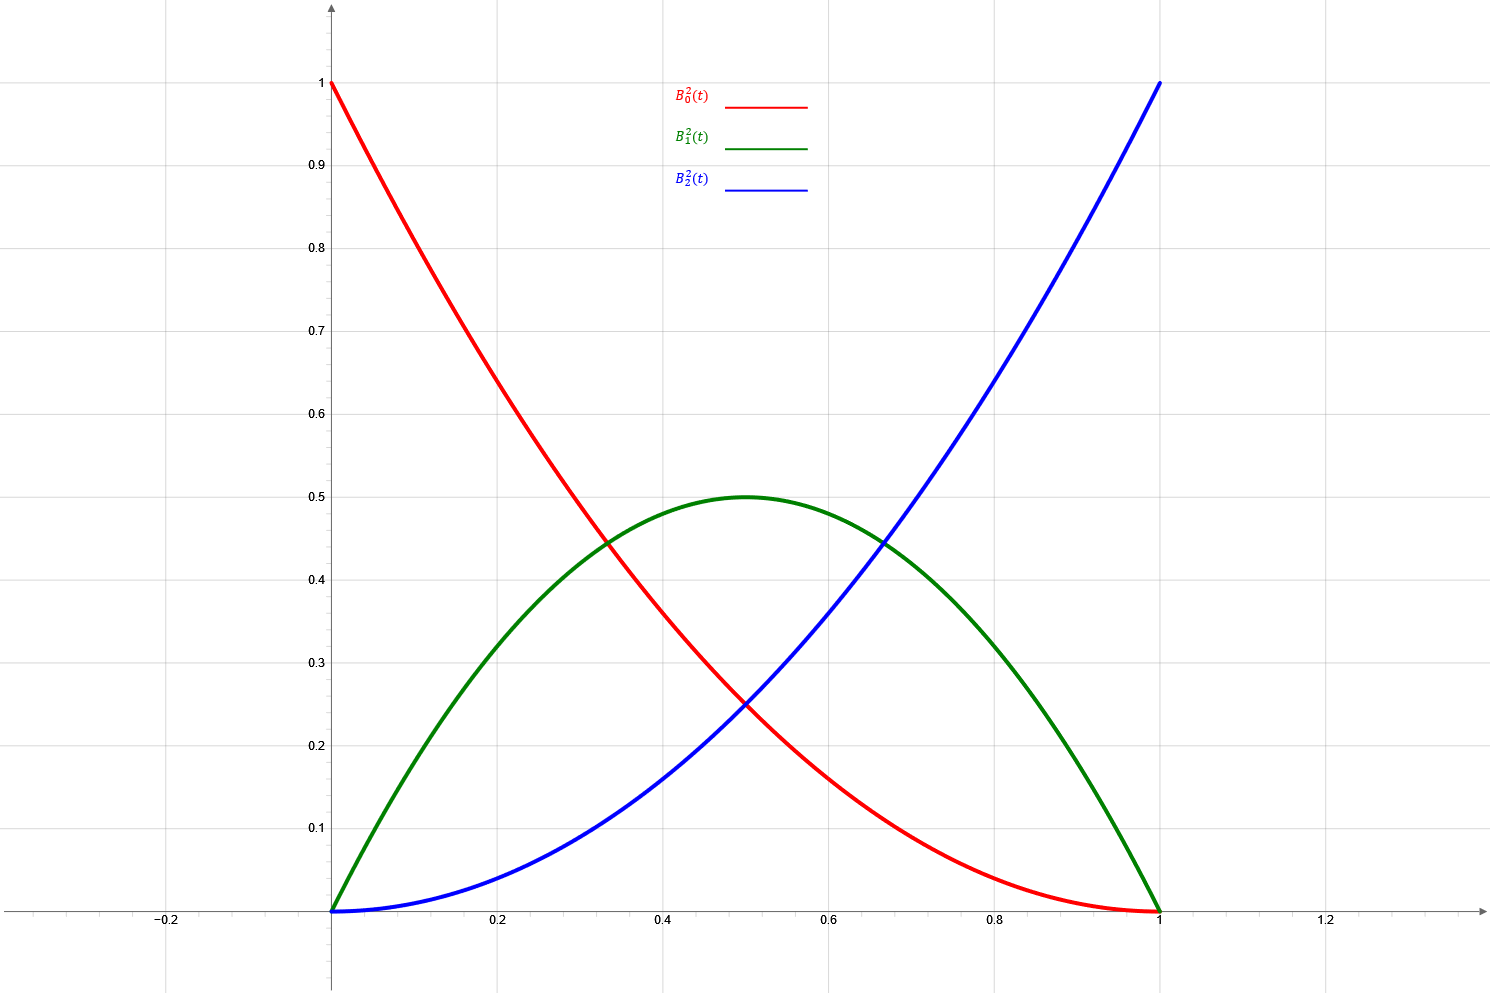
\includegraphics[width = \groupimagewidth]{images/bernstein-2}}
        \qquad
        \subfloat[$n=3$]{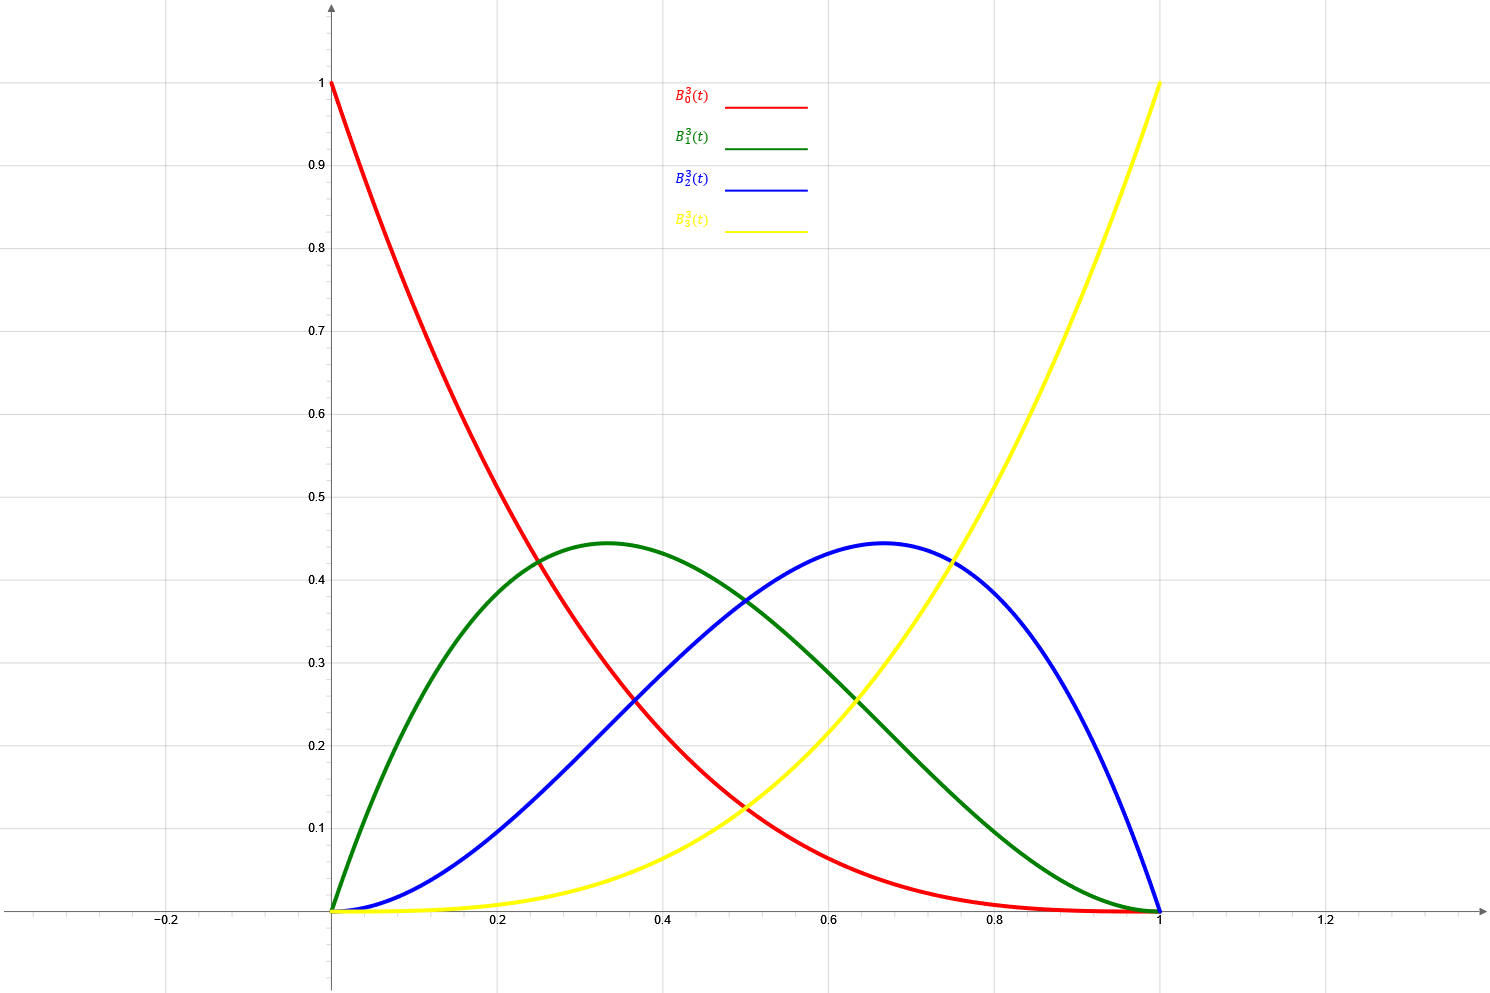
\includegraphics[width = \groupimagewidth]{images/bernstein-3}}
        \caption{Bernsteinovi bazni polinomi stopenj $n=0,1,2,3$.}
        \label{fig:bernstein-base}
    \end{figure}
    Brez dokaza v naslednjem izreku naštejmo nekaj osnovnih lastnosti Bernsteinovih baznih polinomov.
    \begin{izrek}
        Za Bernsteinove bazne polinome $B_i^n$ veljajo naslednje lastnosti.
        \label{izrek:bernsteinovi_lastnosti}
        \begin{enumerate}
            \item So nenegativni na intervalu $[0,1]$.\label{izrek:bernsteinovi_lastnosti:pozitivnost}
            \item $B_i^n(0) = \delta_{i,0}$ in $B_i^n(1) = \delta_{i,n}$, kjer je $\delta_{i,j} = \begin{cases}
                                                                                                      1, & i=j, \\
                                                                                                      0, & 1\neq j.
            \end{cases}.$
            \item So simetrični, tj.\ $B_i^n(1-t) = B^n_{n-i}(t)$, $t\in\R$. \label{izrek:bernsteinovi_lastnosti:simetrija}
            \item Tvorijo razčlenitev enote, tj.\  $\sum_{i=0}^{n}B_{i}^{n}(t) = 1$, $t\in\R$.\label{izrek:bernsteinovi_lastnosti:enota}
        \end{enumerate}
    \end{izrek}
%    \begin{dokaz}
%        Lastnost (1) očitno izhaja iz lastnosti binomskega simbola, lastnost (2) pa iz definicije.
%        Dokažimo simetričnost in razčlenitev enote.\\
%        \noindent(3) Namesto spremenljivke $t$ v enačbo za bernsteinov bazni polinom $B_i^n(t)$ vstavimo izraz $1-t$ in uporabimo lastnost binomskega simbola $\binom{n}{i} = \binom{n}{n-i}$, dobimo
%        \[B_i^n(1-t) = \binom{n}{i}(1-t)^i(1-(1-t))^{n-i} =  \binom{n}{n-i}(1-t)^it^{n-i} = B^{n-i}_{i}(t).\]
%        \noindent(5) Za $1 = 1^n = (1-t+t)^n = ((1-t) + t)^n$ uporabimo binomski izrek, dobimo
%        \[\left((1-t) + t\right)^n = \sum_{i=0}^{n}\bernstein{n}{i} = \sum_{i=0}^n B_i^n(t).\]
%    \end{dokaz}
    \noindent Prve tri lastnosti iz izreka lahko opazimo na že prej omenjeni sliki~\ref{fig:bernstein-base}.
    Četrto lastnost pa je moč opaziti na sliki~\ref{fig:bernstein-base-sum}, kjer so prikazani naloženi ploščinski grafikoni Bernsteinovih baznih polinomov. % za stopnje $n=0,1,2,3$.
    Količina barve pri določenem parametru $t\in[0,1]$ pove, koliko pripadajoč polinom $B_i^n$ prispeva k razčlenitvi enote.
    \begin{figure}[h]
        \captionsetup[subfigure]{labelformat=empty}
        \centering
        \subfloat[$n=0$]{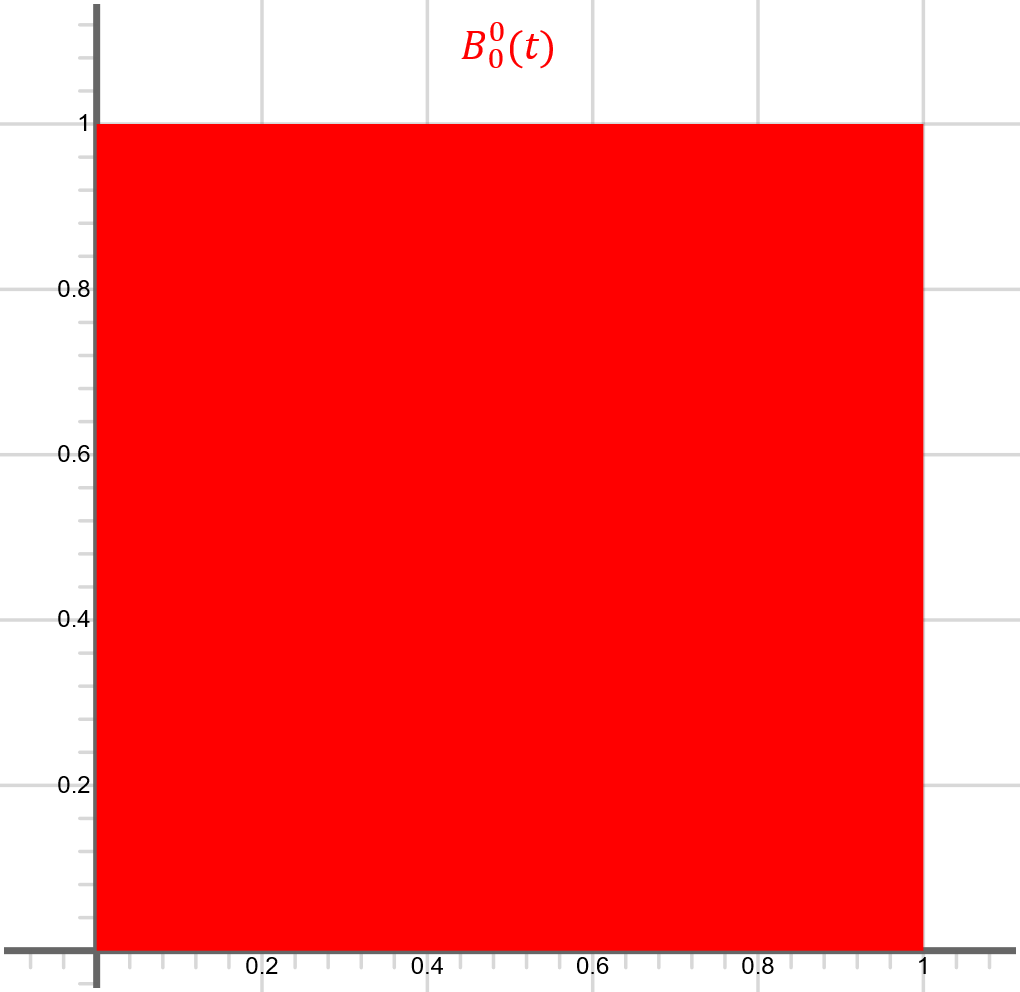
\includegraphics[width = \groupimagewidth]{images/bernstein-sum-0}}
        \qquad
        \subfloat[$n=1$]{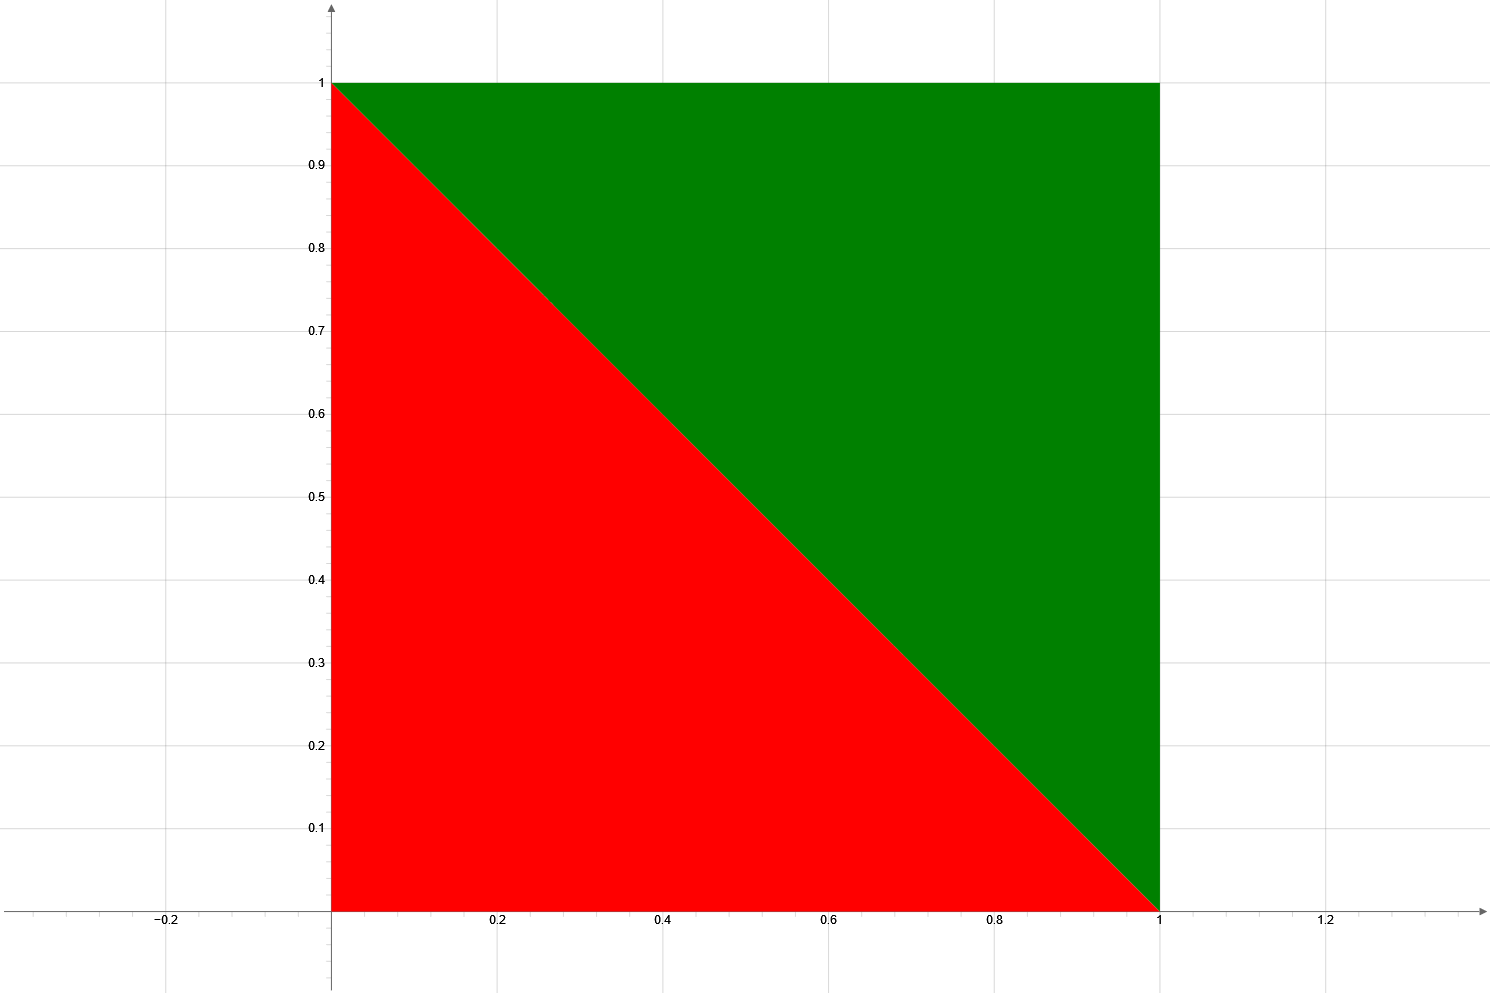
\includegraphics[width = \groupimagewidth]{images/bernstein-sum-1}} \\
        \subfloat[$n=2$]{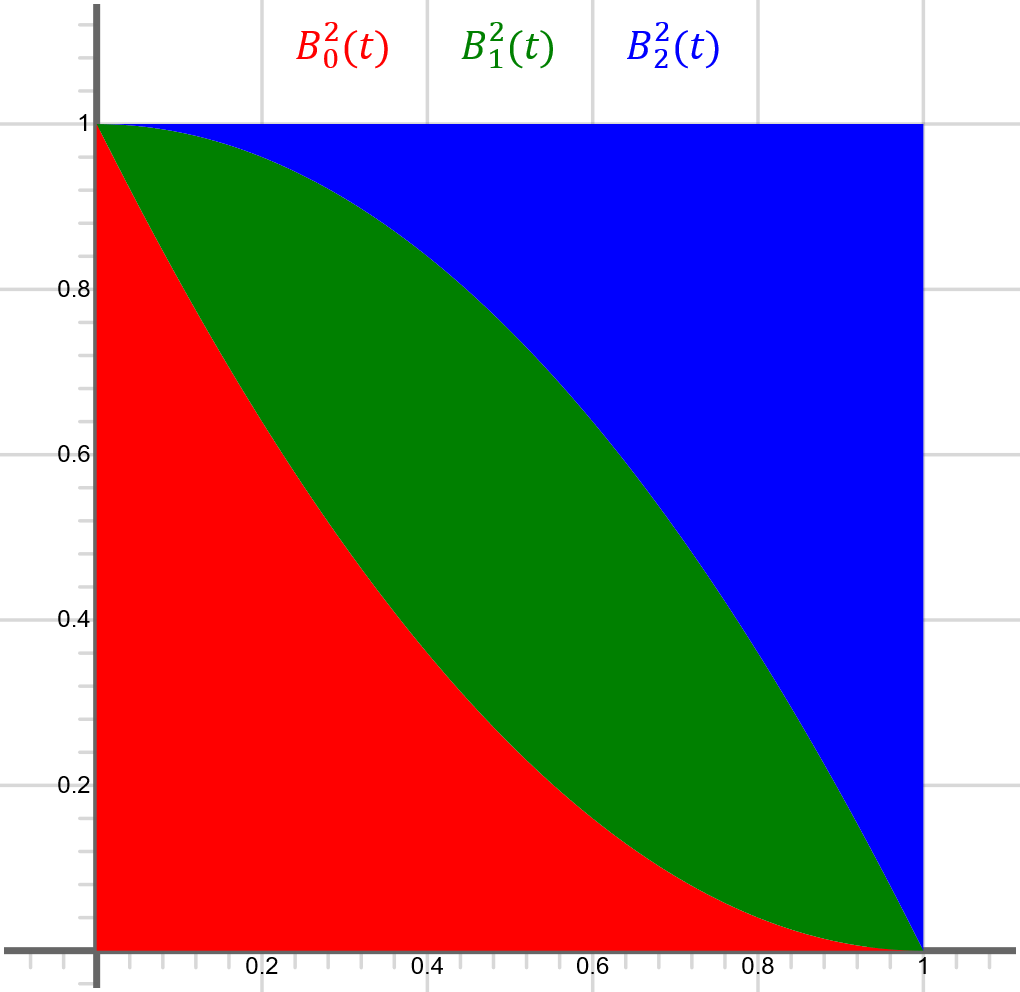
\includegraphics[width = \groupimagewidth]{images/bernstein-sum-2}}
        \qquad
        \subfloat[$n=3$]{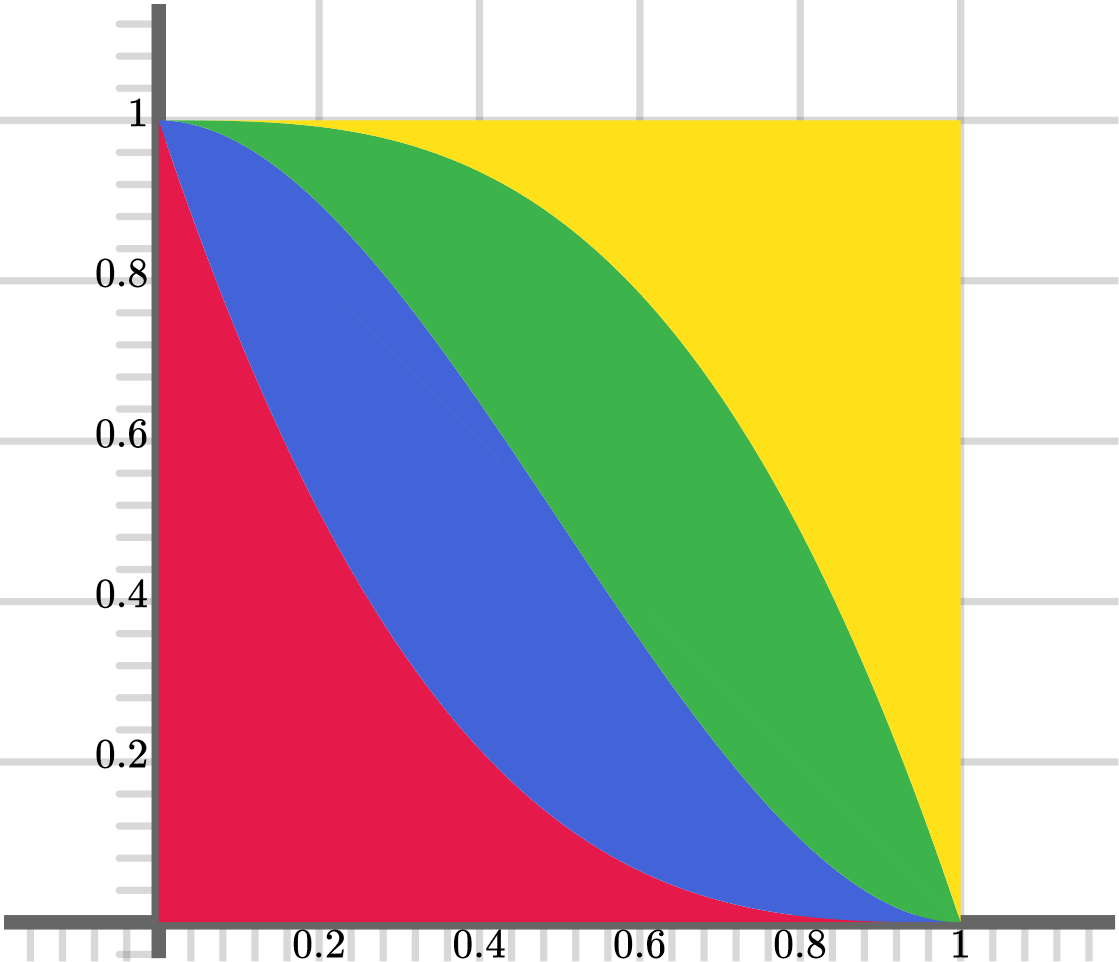
\includegraphics[width = \groupimagewidth]{images/bernstein-sum-3}}
        \caption{Naloženi ploščinski grafikoni Bernsteinovih baznih polinomov.}
        \label{fig:bernstein-base-sum}
    \end{figure}

    S sledečim izrekom podamo rekurzivno zvezo za računanje vrednosti Bernsteinovih baznih polinomov.
    \begin{izrek}
        \label{izrek:bernsteinovi_lastnosti:rekruzija}
        Za Bernsteinove bazne polinome stopnje $n\geq1$ velja rekurzivna zveza
        \[B_i^n(t) = (1-t)B_i^{n-1}(t) + tB_{i-1}^{n-1}(t),\ t\in\R.\]
    \end{izrek}
    \noindent Izrek je enostavno dokazati s pomočjo indukcije, zato bomo dokaz izpustili.
%    Rekurzivno zvezo dokažimo z indukcijo.
%    \begin{dokaz}
%        Za $n=1$ zveza drži, saj iz nje dobimo $B_i^1(t) = (1-t)B_i^{0}(t) + tB_{i-1}^{0}(t)$ oziroma $B_0^1(t) = (1-t)$ in $B_1^1(t) = t$.
%        Za indukcijski korak pa desni del rekurzivne zveze manipuliramo, da pridemo do levega
%        \begin{align*}
%        (1-t)
%            B_i^{n-1}(t) + tB_{i-1}^{n-1}(t) &= \binom{n-1}{i}t^{i}(1-t)^{n-i} + \binom{n-1}{i-1}t^{i}(1-t)^{n-i}  \\
%            &\stackrel{(1)}{=} \binom{n}{i}t^{i}(1-t)^{n-i} = B_i^n(t),
%        \end{align*}
%        kjer smo pri enakosti (1) uporabili lastnost binomskega simbola $\binom{n-1}{i} + \binom{n-1}{i-1} = \binom{n}{i}.$
%    \end{dokaz}
    V kasnejših razdelkih bomo potrebovali tudi odvode Bernsteinovih baznih polinomov.
    Ker Bernsteinovi bazni polinomi stopnje $n$ tvorijo bazo prostora $\mathbb{P}_n$, lahko njihove odvode izrazimo v Bernsteinovi bazi dimenzije $n-1$.
    Z nekaj računanja pridemo do sledečega rezultata.
    \begin{izrek}
        \label{izrek:bernstein-odvod}
        Za odvode Bernsteinovih baznih polinomov velja zveza
        \[B_{i}^{n\prime}=n(B_{i-1}^{n-1} - B_{i}^{n-1}).\]
    \end{izrek}
%    \begin{dokaz}
%        Bernsteinov bazni polinom najprej odvajamo da dobimo
%        \begin{align*}
%            B_{i}^{n\prime}(t) &=\binom{n}{i}\left(it^{i-1}(1-t)^{n-i} - (n-i) t^i(1-t)^{n-i-1} \right) \\
%            &=\binom{n}{i}it^{i-1}(1-t)^{n-i} - \binom{n}{i}(n-i) t^i(1-t)^{n-i-1}.
%        \end{align*}
%        Nato v zgornje vstavimo binomski zvezi $\binom{n}{i}i = \frac{n!i}{(n-i)i!} =  \frac{n(n-1)!}{(n-i)(i-1)!} = n\binom{n-1}{i-1}$ in $\binom{n}{i}(n-i) = \frac{n!(n-i)}{(n-i)!}  = \frac{n(n-1)!}{(n-i-1)!} =n\binom{n-1}{i}$ in dobimo željeno.
%    \end{dokaz}
    Za konec podrazdelka izpeljimo še formulo za zmnožek dveh Bernsteinovih polinomov.
    \begin{izrek}
        Naj bosta $f$ in $g$ Bernsteinova polinoma definirana kot $f=\sum_{i=0}^{m}\alpha_iB_i^m$ in $g=\sum_{i=0}^{n}\beta_iB_i^n$.
        Potem za njun zmnožek velja
        \[ fg = \sum_{i=0}^{m+n}\left(\sum_{j=\max(0,i-n)}^{\min(m,i)} \frac{\binom{m}{j}\binom{n}{i-j}}{\binom{m+n}{i}} \alpha_i\beta_{i-j} \right)B_{i}^{m+n}.\]
    \end{izrek}
    \begin{dokaz}
        Naj bosta $f$ in $g$ Bernsteinova polinoma iz predpostavk izreka.
        Polinoma zmnožimo in dobimo
        \[fg =\sum_{i=0}^{m}\alpha_iB_{i}^{m}\sum_{j=0}^{n}\beta_jB_{j}^{n} = \sum_{i=0}^{m+n}\sum_{l=0}^i \alpha_lB_{l}^{m}\beta_{i-l}B_{i-l}^{n}. \]
        V zadnji izraz vstavimo funkcijske predpise Bernsteinovih baznih polinomov, ga poenostavimo in dobimo
        %&= \sum_{i=0}^{m+n}\sum_{l=0}^i \alpha_l \binom{m}{l}t^{l}(1-t)^{m-l} \beta_{i-l} \binom{n}{i-l}t^{i-l}(1-t)^{n-i+l} \\
        \[\sum_{i=0}^{m+n}\sum_{l=0}^i \alpha_l \beta_{i-l} \binom{m}{l}\binom{n}{i-l}t^{i}(1-t)^{m+n-i}.\]
        Kar lahko z izpostavitvijo binoma $\binom{m+n}{i}$ predstavimo v Bernsteinovi bazi kot
        \[\sum_{i=0}^{m+n} \left(\sum_{l=0}^i  \alpha_l \beta_{i-l}\frac{\binom{m}{l}\binom{n}{i-l}}{\binom{m+n}{i}}\right) B_{i}^{m+n}.\]
        V primerih, ko velja $l>m$ ali $i-l>n$ imamo v števcu ulomka $0$, kar privede do zapisa iz izreka.
    \end{dokaz}

    \subsection{Večdimenzionalne oznake}
    Da bodo zapisi v sledečih razdelkih bolj pregledni, bomo uvedli večdimenzionalne oznake.
%    Večdimenzionalnost bomo ponazarjali z odebelitvijo črke.
    Točke v večdimenzionalnem prostoru bomo označili z odebeljenimi črkami, na primer $\mathbf{x}=(x_0,x_1,\dots,x_n)\in\R^{n+1}$.
    Podobno bomo odebelili črke funkcij, ki v večdimenzionalni prostor slikajo, na primer $\mathbf{f}:\R\to\R^{n+1}$.
%    Tako bomo večdimenzionalnost točke $x\in\R^{n+1}$ označili z $\mathbf{x}=(x_0,x_1,\dots,x_n)$, večdimenzionalnost funkcije $f:\R\to\R^{n+1}$ pa z $\mathbf{f}=\left( f_0,f_1,\dots,f_n\right)$.

    \subsection{Bézierjeve krivulje}
    Če v Bernsteinovem polinomu skalarne koeficiente zamenjamo s točkami, dobimo predpis parametrizacije Bézierjeve krivulje.
    \begin{definicija}
        Bézierjeva krivulja $\mathbf{B}: [0,1]\to \R^d$ stopnje $n\in\N$ je polinomska krivulja podana s točkami $\p_i\in\R^d$,  $i=0,1,\ldots,n$, in parametrizacijo
        \[\mathbf{B}=\bernsteinsump{i}{n}.\]
        Točkam $\p_i$ pravimo \textit{kontrolne točke}.
        Če zaporedne kontrolne točke povežemo, dobimo \textit{kontrolni poligon}.
    \end{definicija}
    \begin{opomba}
        \label{opomba:dim-0}
        Kjer je potrebno, lahko definicijo razširimo tudi na stopnjo $n=0$.
        Iz zgornje parametrizacije potem sledi $\mathbf{B}(t)=\p_0$.
    \end{opomba}
    \begin{opomba}
        Pri slikovnem gradivu iz dela se bomo omejili na prostor dimenzije $d=2$, torej na Bézierjeve krivulje v ravnini.
    \end{opomba}
    \noindent Na sliki~\ref{fig:bezierjeva-krivulja} si lahko ogledamo primere Bézierjevih krivulj stopenj $n=1,2,3,4$ s pripadajočimi kontrolnimi poligoni.
    \begin{figure}[ht]
        \captionsetup[subfigure]{labelformat=empty}
        \centering
        \subfloat[$n=1$]{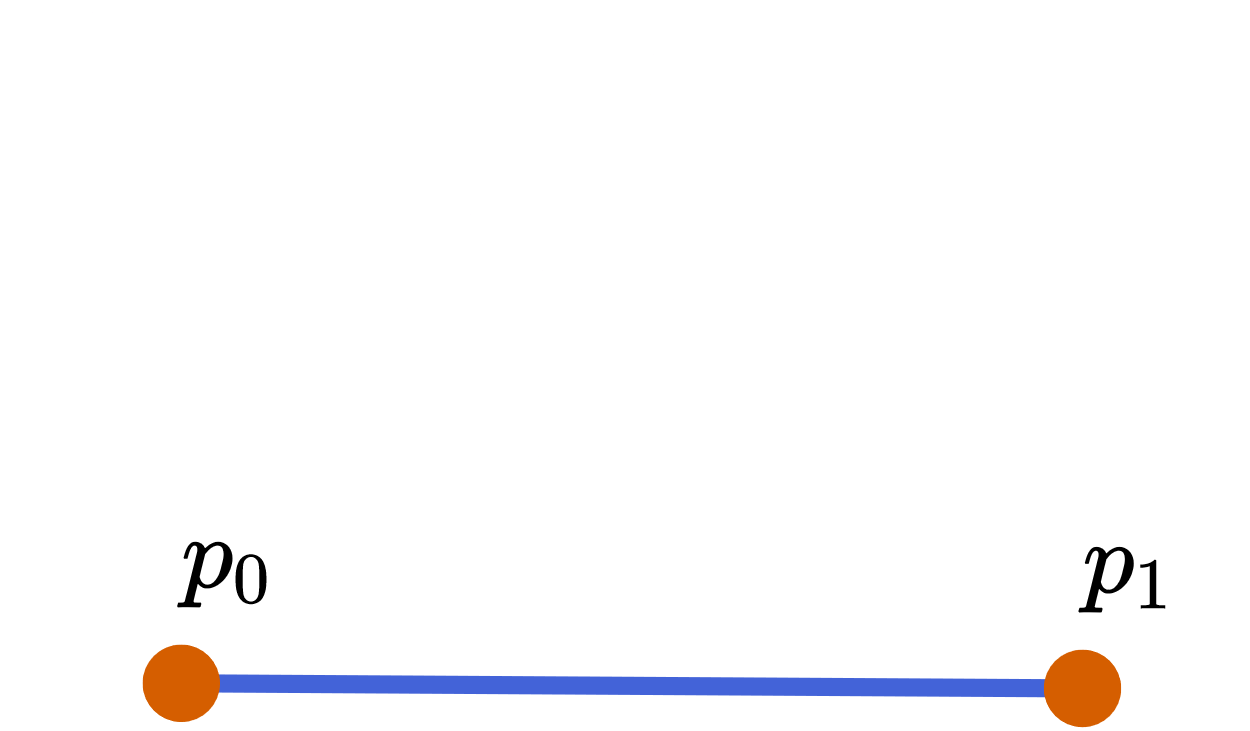
\includegraphics[width = \groupimagewidth]{images/bezier-curve-1}}
        \qquad
        \subfloat[$n=2$]{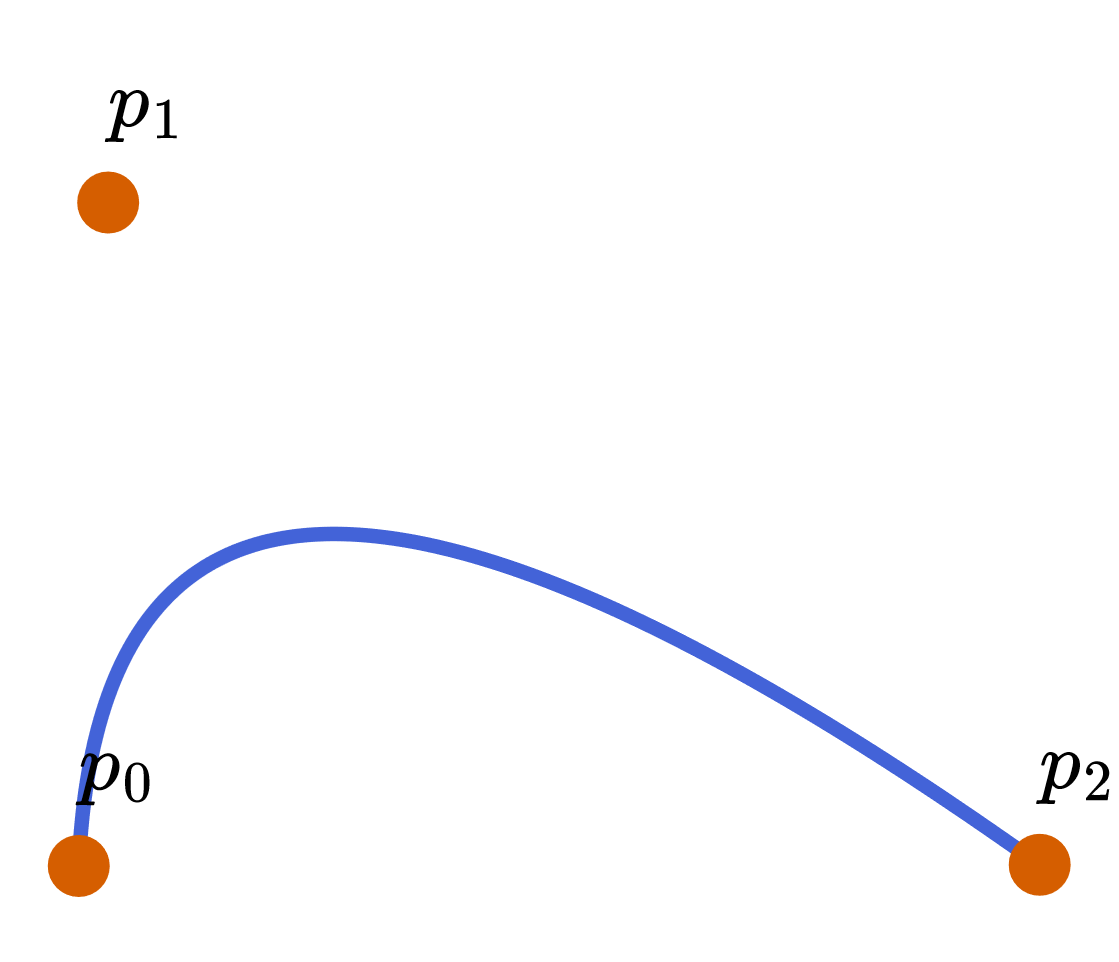
\includegraphics[width = \groupimagewidth]{images/bezier-curve-2}} \\
        \subfloat[$n=3$]{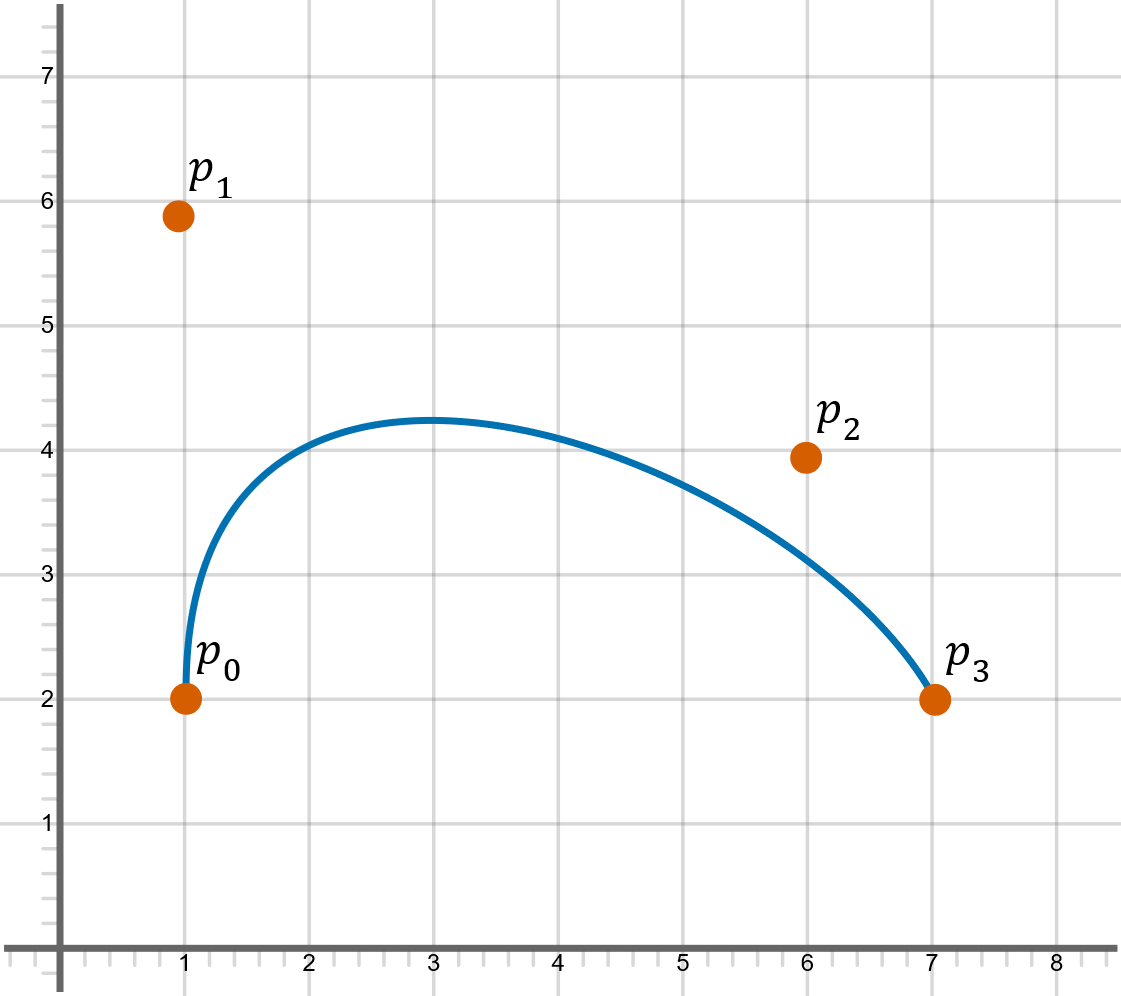
\includegraphics[width = \groupimagewidth]{images/bezier-curve-3}}
        \qquad
        \subfloat[$n=4$]{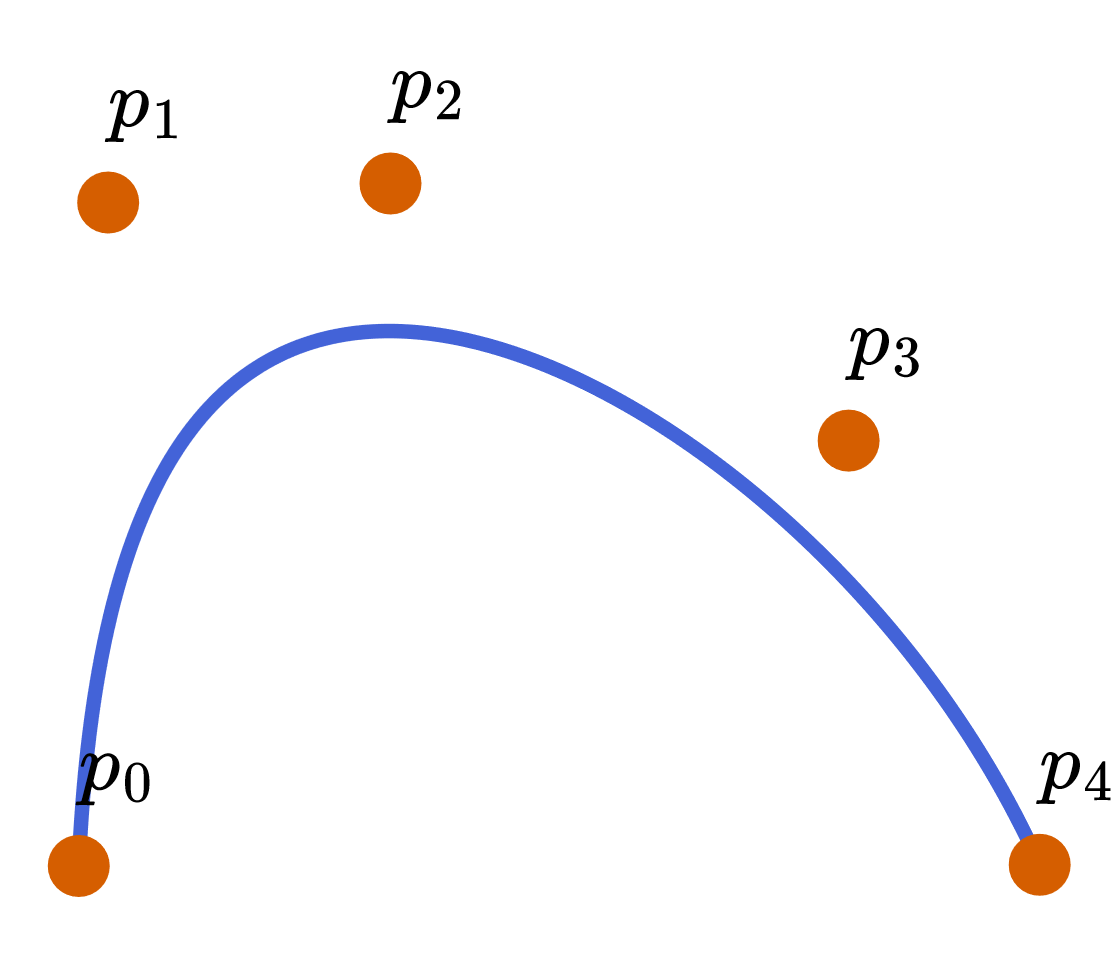
\includegraphics[width = \groupimagewidth]{images/bezier-curve-4}}
        \caption{Bézierjeve krivulje s pripadajočimi kontrolnimi poligoni za stopnje $n=1,2,3,4$.}
        \label{fig:bezierjeva-krivulja}
    \end{figure}

    Zapišimo sedaj nekaj osnovnih lastnosti Bézierjevih krivulj.
    \begin{izrek}{Bézierjeva krivulja $\mathbf{B}$ s kontrolnimi točkami $\p_i$, $i=0,1\ldots,n$, ima sledeče lastnosti.}
        \label{izrek:lastnosti-bezierjevih-krivulj}
        \begin{enumerate}
            \item Interpolira končni točki, tj.\ velja $\mathbf{B}(0)=\p_0$ in $\mathbf{B}(1)=\p_n$.
            \item Je afino invariantna, tj.\ za poljubno afino transformacijo $A$ velja \[A \left(\bernsteinsump{i}{n}\right) =\bernsteinsumtritri{i}{n}{A(\p_i)}.\]
            \item Leži znotraj konveksne ovojnice svojih kontrolnih točk.
        \end{enumerate}
    \end{izrek}
    \noindent Dokazi lastnosti so enostavni, zato jih izpustimo.
    Preden si lastnosti ogledamo na slikah, povejmo zakaj so pomembne za CAGD sisteme.
    Interpolacija končnih točk uporabniku omogoča kontrolo nad tem, kje se bo krivulja začela in kje zaključila.
    Zaradi afine invariance lahko uporabnikove transformacije krivulje v ozadju CAGD sistema prevedemo v transformacije kontrolnih točk.
    Tretja lastnost pa uporabniku s kontrolnimi točkami omogoča upravljanje krivulje, kjer je krivulja zmerom v bližini svojih kontrolnih točk.
    Lastnosti si sedaj oglejmo na slikah.
    Interpolacijo končnih točk je bilo moč videti že na sliki~\ref{fig:bezierjeva-krivulja}.
    Posledice afine invariance si lahko ogledamo na sliki~\ref{fig:bezier-affine-transform}.
    Na sliki~\ref{fig:bezier-convex-hull} pa si lahko ogledamo konveksni ovojnici kontrolnih točk dveh Bézierjevih krivulj.
    Vidimo, da krivulji ležita znotraj njih.
    \begin{figure}[ht!]
        \captionsetup[subfigure]{labelformat=empty}
        \centering
        \subfloat[začetna krivulja]{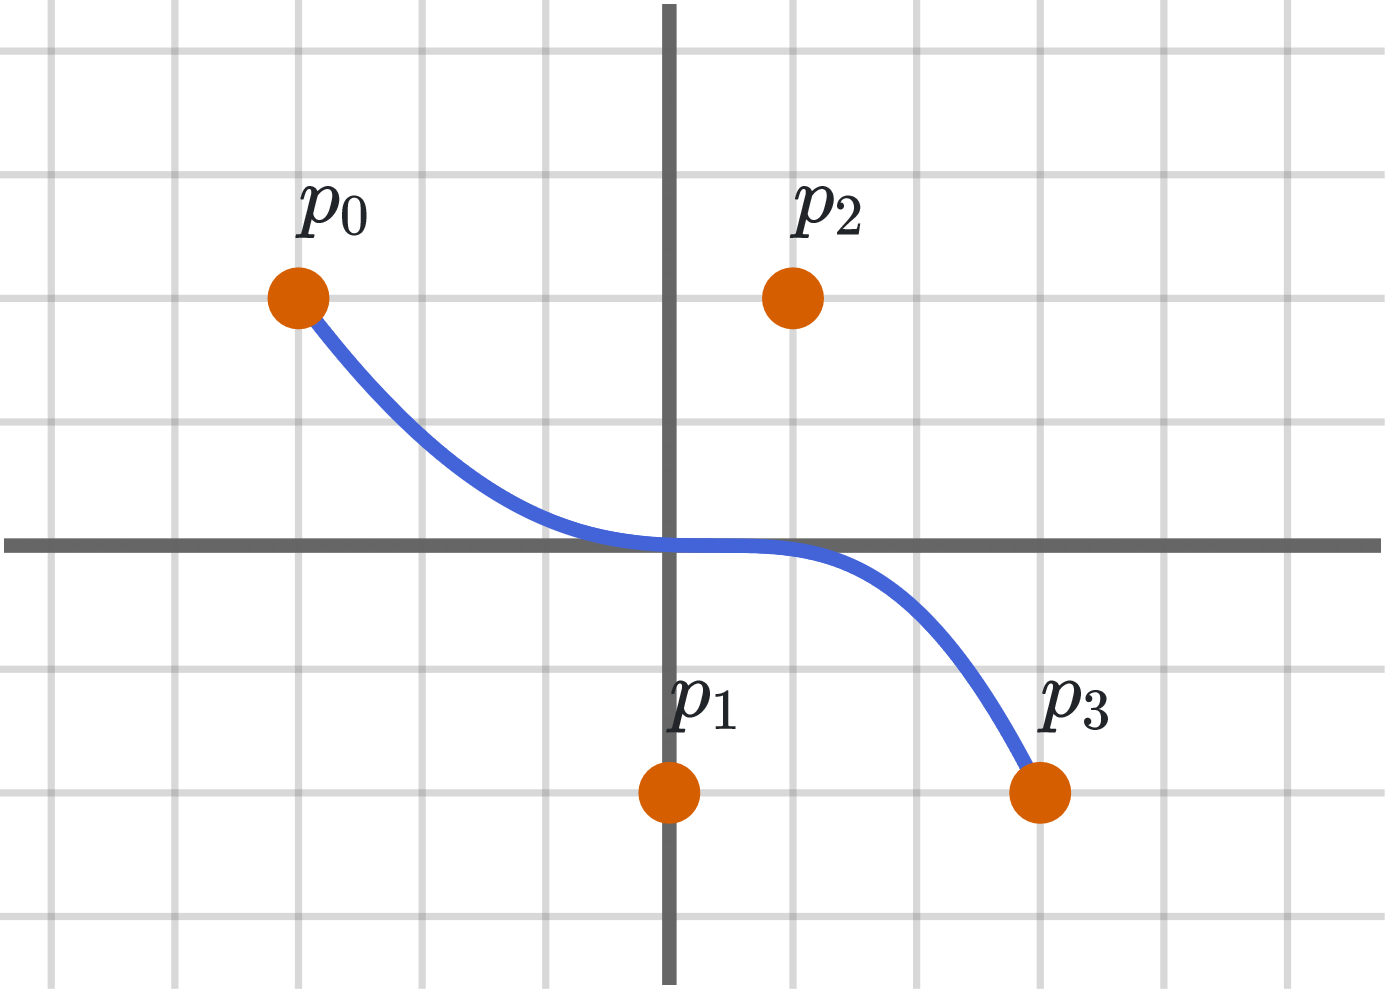
\includegraphics[width = \groupimagewidth]{images/afine-transform-start}}
        \qquad
        \subfloat[povečanje]{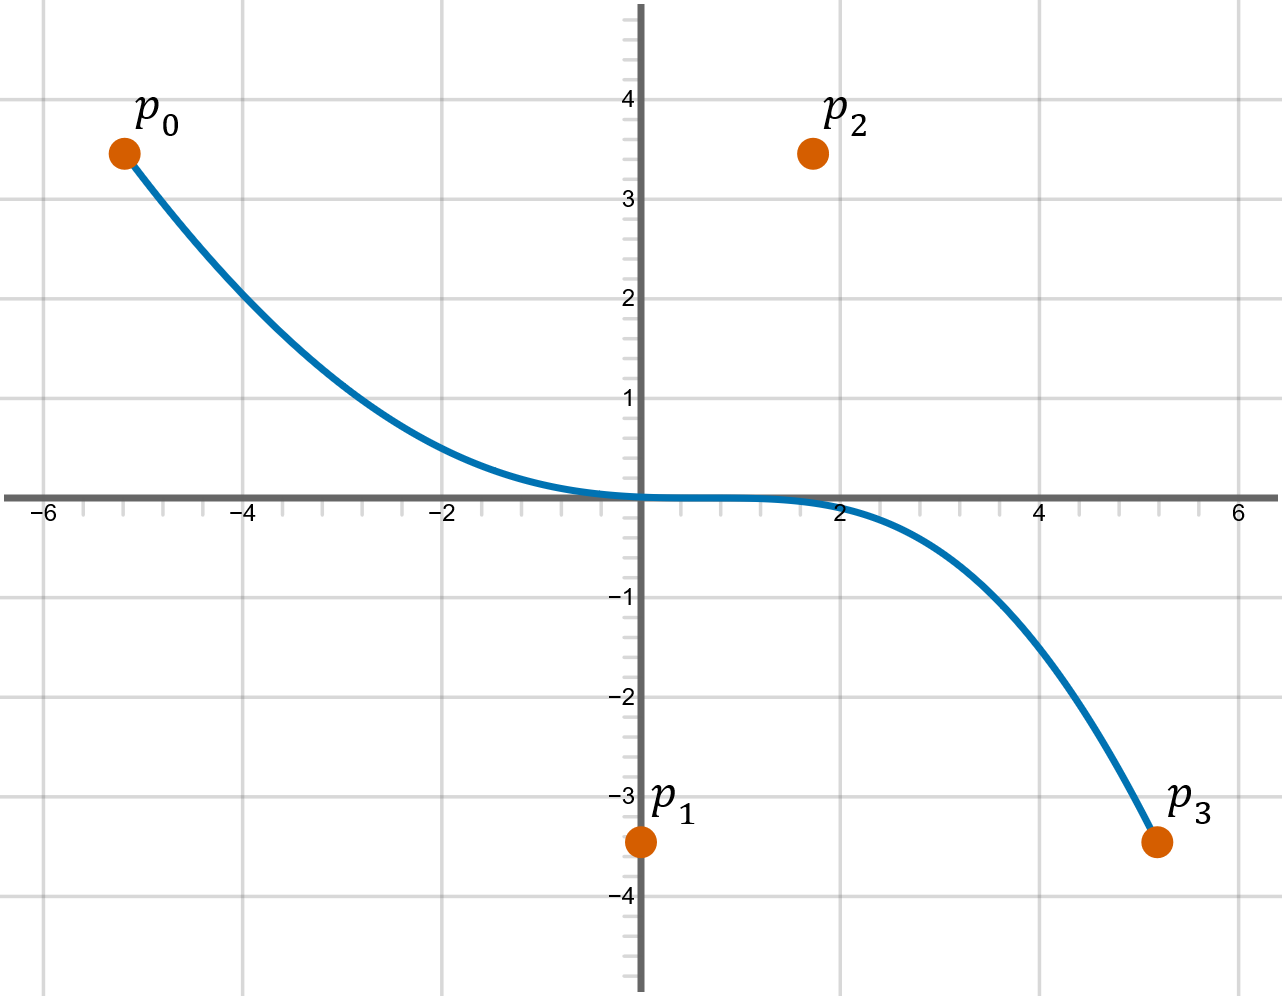
\includegraphics[width = \groupimagewidth]{images/afine-transform-bigger}} \\
        \subfloat[zrcaljenje čez $x$ os]{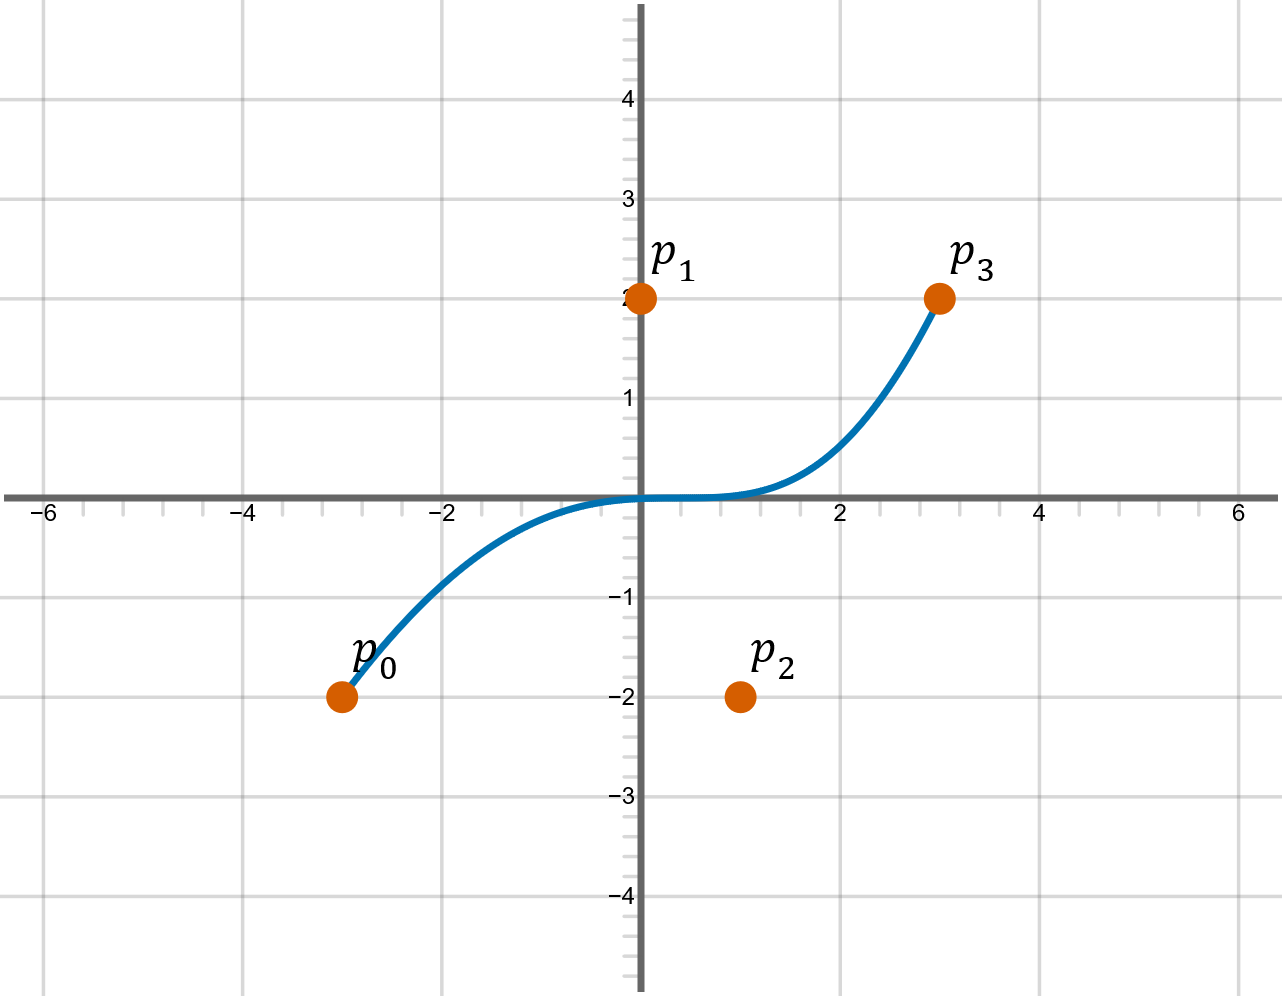
\includegraphics[width = \groupimagewidth]{images/afine-transform-flip}}
        \qquad
        \subfloat[rotiranje za $\frac{\pi}{2}$]{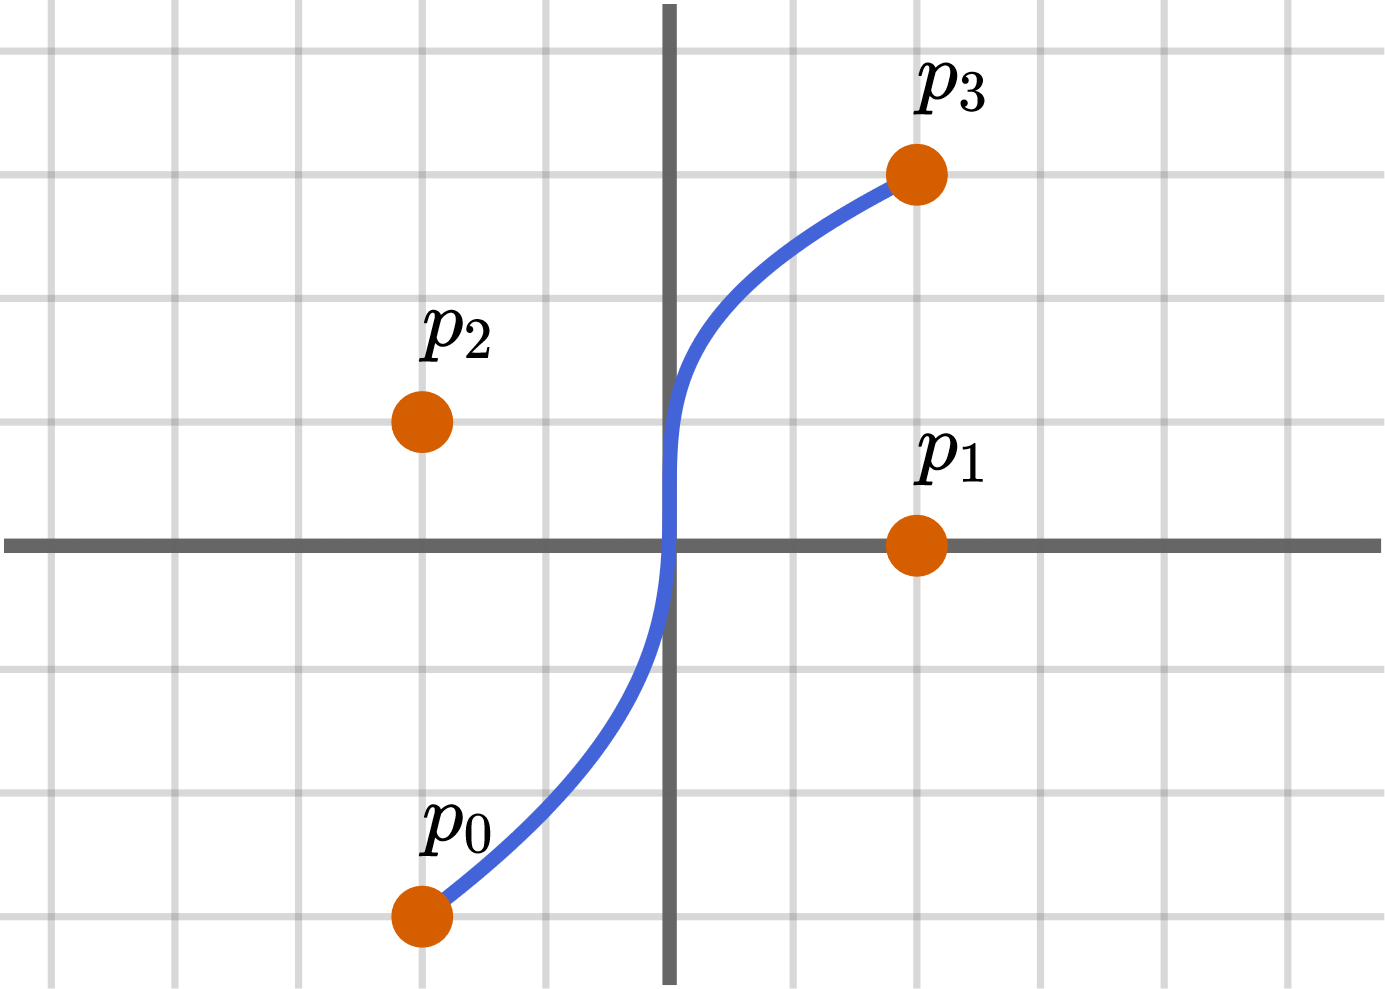
\includegraphics[width = \groupimagewidth]{images/afine-transform-rotate}}
        \caption{Afine transformacije Bézierjeve krivulje.}
        \label{fig:bezier-affine-transform}
    \end{figure}
    \begin{figure}[ht!]
        \captionsetup[subfigure]{labelformat=empty}
        \centering
        \subfloat[]{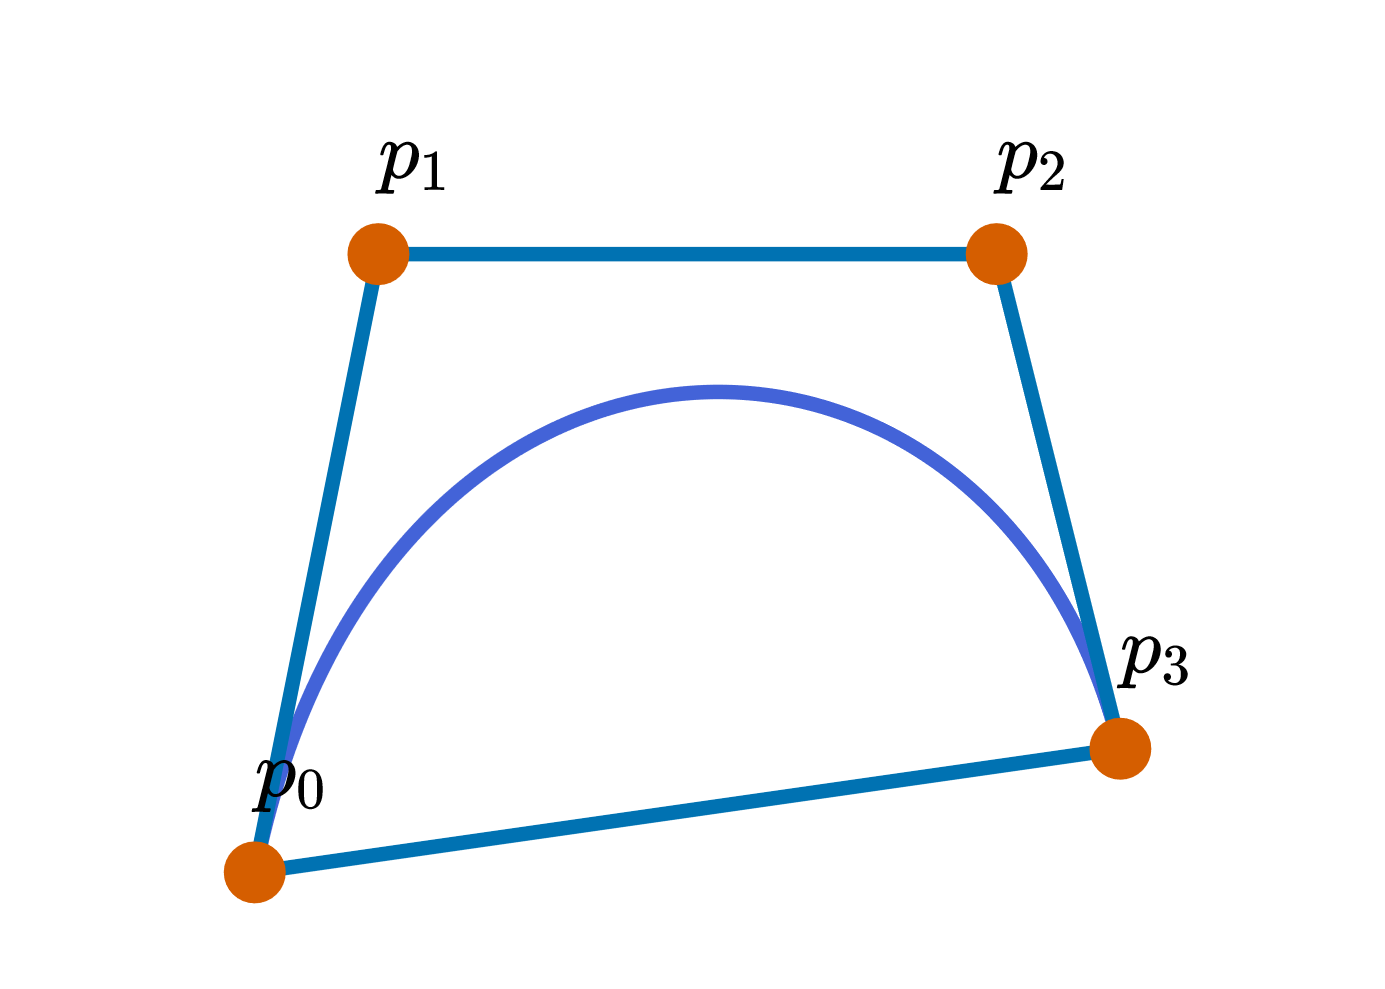
\includegraphics[width = \groupimagewidth]{images/bezier-curve-convex-hull-1}}
        \qquad
        \subfloat[]{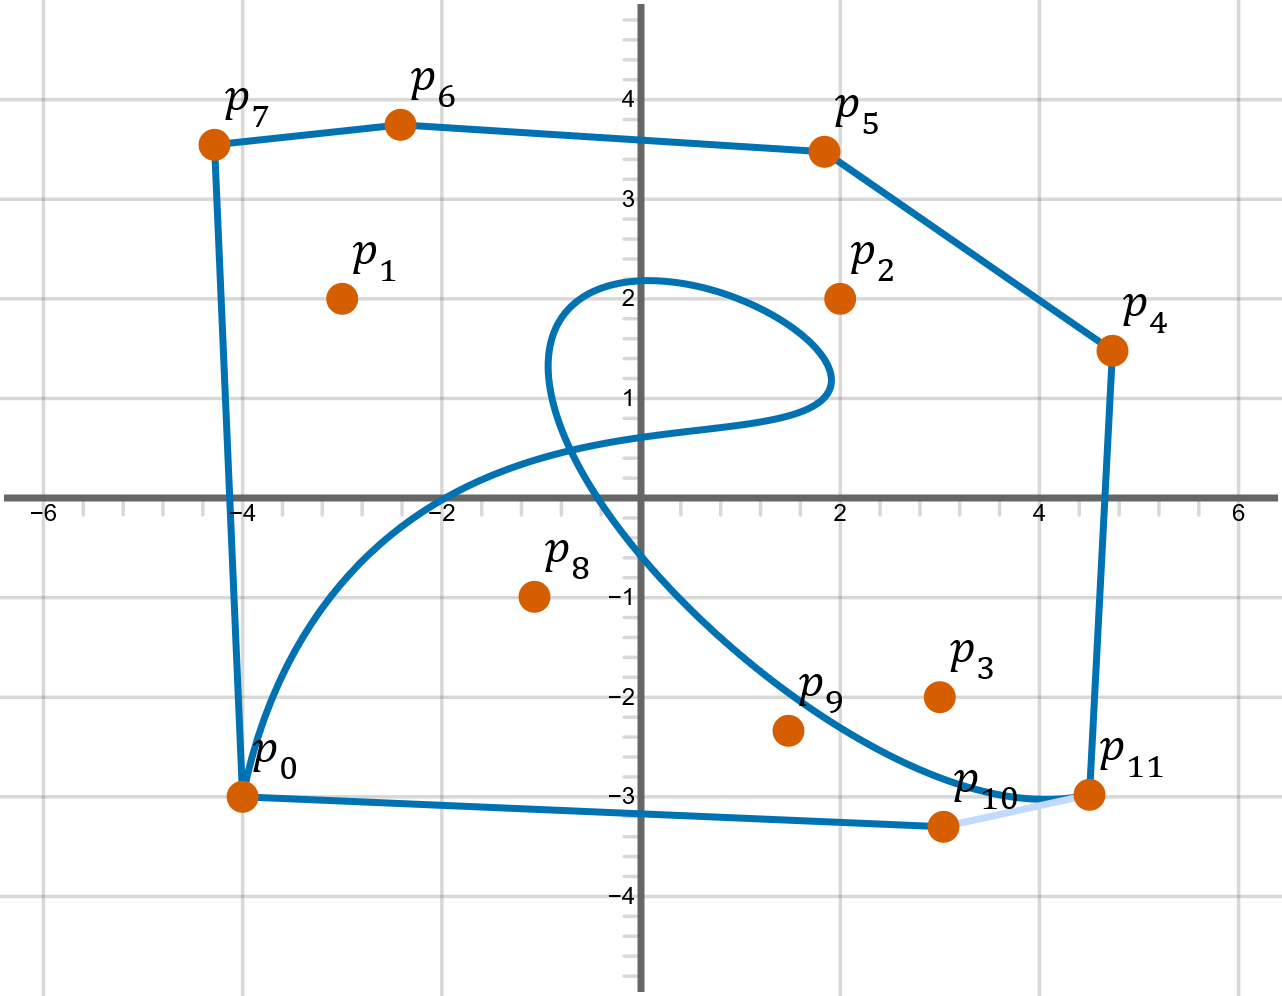
\includegraphics[width = \groupimagewidth]{images/bezier-curve-convex-hull-2}}
        \caption{Konveksni ovojnici kontrolnih točk Bézierjevih krivulj.}
        \label{fig:bezier-convex-hull}
    \end{figure}

%    Izrek~\ref{izrek:lastnosti-bezierjevih-krivulj} sedaj tudi dokažimo.
%    \begin{dokaz}
%        \noindent Lastnost (1) dokažemo s pomočjo izreka~\ref{izrek:bernsteinovi_lastnosti}.
%        Iz njega sledi
%        \[ \bigbbod{n}{0}=\sum_{i=0}^{n}\p_{i}B_i^n(t)(0) = \sum_{i=0}^{n}\p_{i}\delta_{0,i} = \p_0.\]%,\ \text{in} \ \bigbbod{n}{1}=\sum_{i=0}^{n}\p_{i}B_i^n(t)(1) = \sum_{i=0}^{n}\p_{i}\delta_{n,i} = \p_n\]
%        Podobno lahko naredimo tudi za $\bigbbod{n}{1}.$
%        Dokažimo sedaj lastnost (2).
%        Naj bo $\varphi$ afina preslikava.
%        Zanjo torej velja $\varphi(x) = A\mathbf{x} + \mathbf{b}$.
%        Potem za afino transformacijo Bézierjeve krivulje velja
%        \begin{align*}
%            \varphi\left(\sum_{i=0}^{n}\p_{i}B_i^n(t)(t)\right) &= A\left(\sum_{i=0}^{n}\p_{i}B_i^n(t)(t)\right) + \mathbf{b} &&=  \sum_{i=0}^{n}A\p_{i}B_i^n(t)(t) + \mathbf{b}  \\
%            &= \sum_{i=0}^{n}A\p_{i}B_i^n(t)(t) + \sum_{i=0}^{n}\mathbf{b}B_i^n(t)(t) &&= \sum_{i=0}^{n}(A\p_{i}+\mathbf{b})B_i^n(t)(t) \\
%            &= \bernsteinsumtritri{i}{n}{\varphi(\p_i).}
%        \end{align*}
%        Kar smo tudi želeli dokazati.
%        Za lastnost (3) posežemo po definiciji konveksne ovojnice.
%        Konveksna ovojnica kontrolnih točk Bézierjeve krivulje je množica vseh konveksnih kombinacij teh točk, tj.\ $\sum_{i=0}^{n}\lambda_i\p_{i}$, kjer so $\lambda_i$ nenegativna realna števila za katere velja $\lambda_0 + \lambda_1 + \dots + \lambda_n = 1$.
%        Ker so Bernsteinovi polinomi razčlenitev enote in nenegativni na intervalu $[0,1]$, lahko zapišemo $\lambda_i=B_i^n(t)$.
%    \end{dokaz}

    \subsection{De Casteljaujev algoritem}
    Stabilnost metod je v CAD in CAGD sistemih bistvene narave.
    Direktno računanje vrednosti Bernsteinovih polinomov preko izrazov iz definicije~\ref{def:bernstein} pa ni stabilno~\ref{placeholder}.
    Da lahko točke Bézierjevih krivulj računamo stabilno, potrebujemo sledeč izrek.
    \begin{izrek}
        \label{izrek:decastelaju-rekurzija}
        Označimo z $\mathbf{B}_{[\p_0,\p_1,\dots,\p_n]}$ Bézierjevo krivuljo s kontrolnimi točkami \\
        $\p_0,\p_1,\dots,\p_n$.
        Potem za poljubno realno število $t$ in naravno število $n$ velja rekurzivna zveza \[\bigbbt_{[\p_0,\p_1,\dots,\p_n]} = (1-t)\bigbbt_{[\p_0,\p_1,\dots,\p_{n-1}]} +t\bigbbt_{[\p_1,\p_2,\dots,\p_n]}.\]
    \end{izrek}
    \noindent Izrek s pomočjo indukcije tudi dokažimo.
    \begin{dokaz}
        Za $n=1$ zveza drži, saj je  \[\bigbbt_{[\p_0,\p_1]} = (1-t)\p_2 +t\p_1 = (1-t)\bigbbt_{[\p_0]} +t\bigbbt_{[\p_1]}.\]
        Indukcijski korak pa dokažemo tako, da v desni del rekurzivne zveze iz izreka vstavimo parametrizaciji Bézierjevih krivulj in dobimo
        \[ (1-t) \bigbbt_{[\p_0,\p_1,\dots,\p_{n-1}]}+t\bigbbt_{[\p_1,\p_2,\dots,\p_n]} = (1-t)\bernsteinsump{i}{n-1}+t\sum_{i=0}^{n-1} \p_{i+1}B_i^{n-1}(t).\]
        Nato zamaknemo indeks desne vsote in skupne točke postavimo pod eno vsoto.
        Od tod sledi
        \begin{align*}
            &(1-t)\bernsteinsump{i}{n-1}+ t\sum_{i=1}^{n} \p_{i}B_{i-1}^{n-1}(t) \\
            %  &= \p_0(1-t)B_{0}^{n-1}(t) + \sum_{i=1}^{n-1}\p_{i}(1-t)B_i^{n-1}(t) +  \sum_{i=1}^{n-1} \p_{i}tB_{i-1}^{n-1}(t) + \p_n B_{n-1}^{n-1}(t) \\
            &= \p_0(1-t)B_{0}^{n-1}(t) + \sum_{i=1}^{n-1}\left((1-t)B_i^{n-1}(t) + tB_{i-1}^{n-1}(t)\right)\p_{i} + \p_n B_{n-1}^{n-1}(t). \\
        \end{align*}
        Uporabimo še rekurzivno zvezo Bernsteinovih baznih polinomov iz izreka~\ref{izrek:bernsteinovi_lastnosti:rekruzija}, da dobimo
        \begin{align*}
            \p_0B_{0}^{n}(t) + \sum_{i=1}^{n-1}\p_{i}B_i^n(t) + \p_n B_{n}^{n}(t) = \sum_{i=0}^{n}\p_{i}B_i^n(t).
        \end{align*}
    \end{dokaz}
    \noindent Na sliki~\ref{fig:decasteljau-2} lahko vidimo, kako lahko točke Bézierjeve krivulje $\mathbf{B}_{[\p_0,\p_1,\p_2,\p_3,\p_4]}$ računamo s pomočjo točk Bézierjevih krivulj $\mathbf{B}_{[\p_0,\p_1,\p_2,\p_3]}$ in $\mathbf{B}_{[\p_1,\p_2,\p_3,\p_4]}$.
    \begin{figure}[h]
        \captionsetup[subfigure]{labelformat=empty}
        \centering
        \subfloat[$t=0.25$]{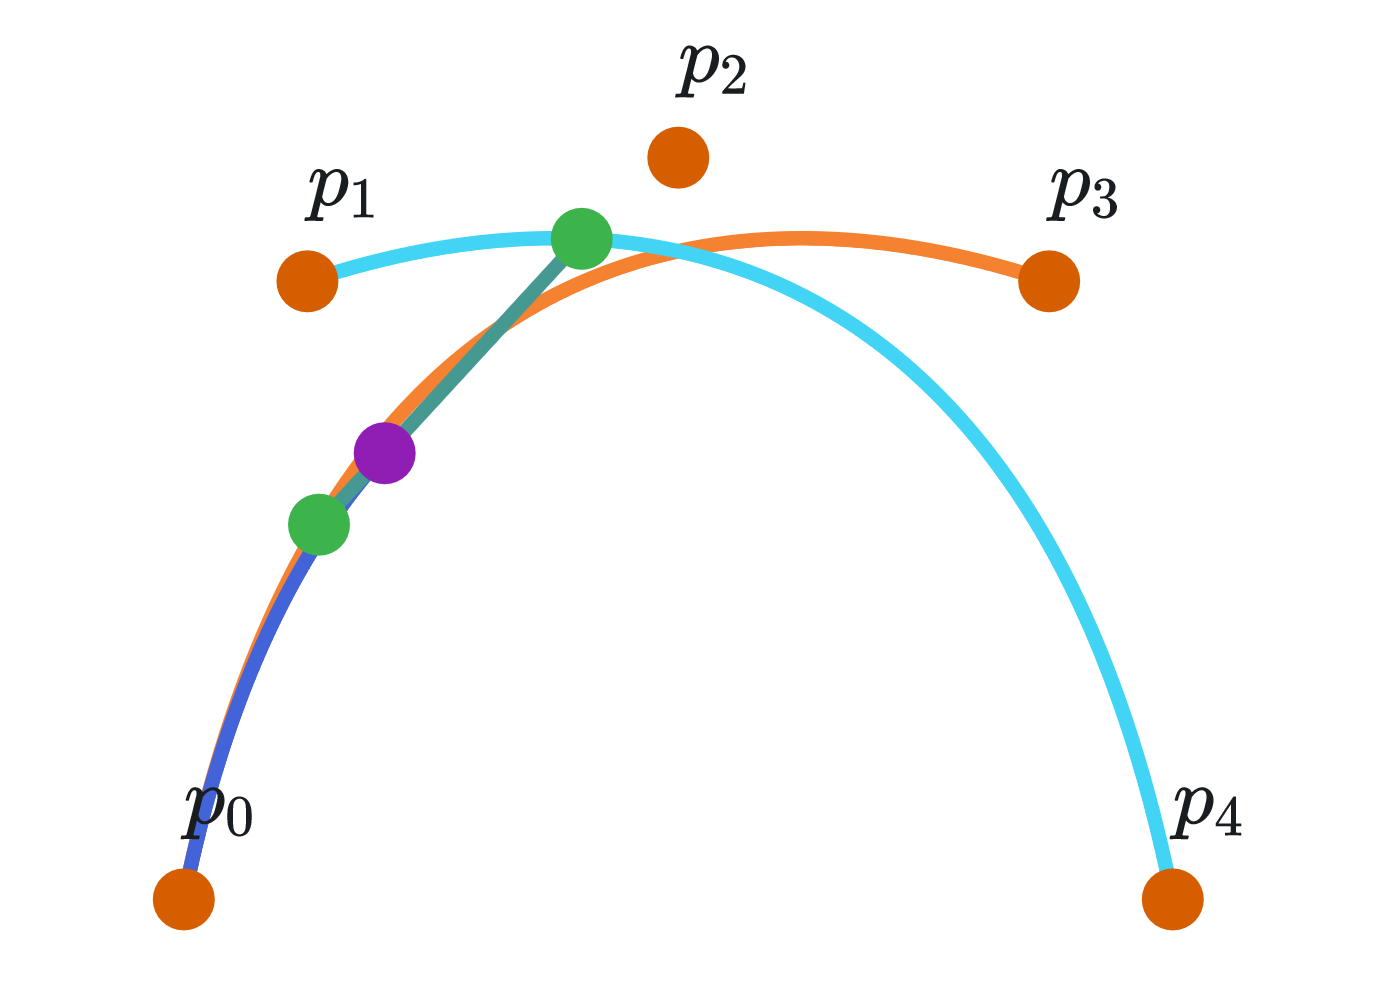
\includegraphics[width = \groupimagewidth]{images/decasteljau-2-t-025}}
        \qquad
        \subfloat[$t=0.5$]{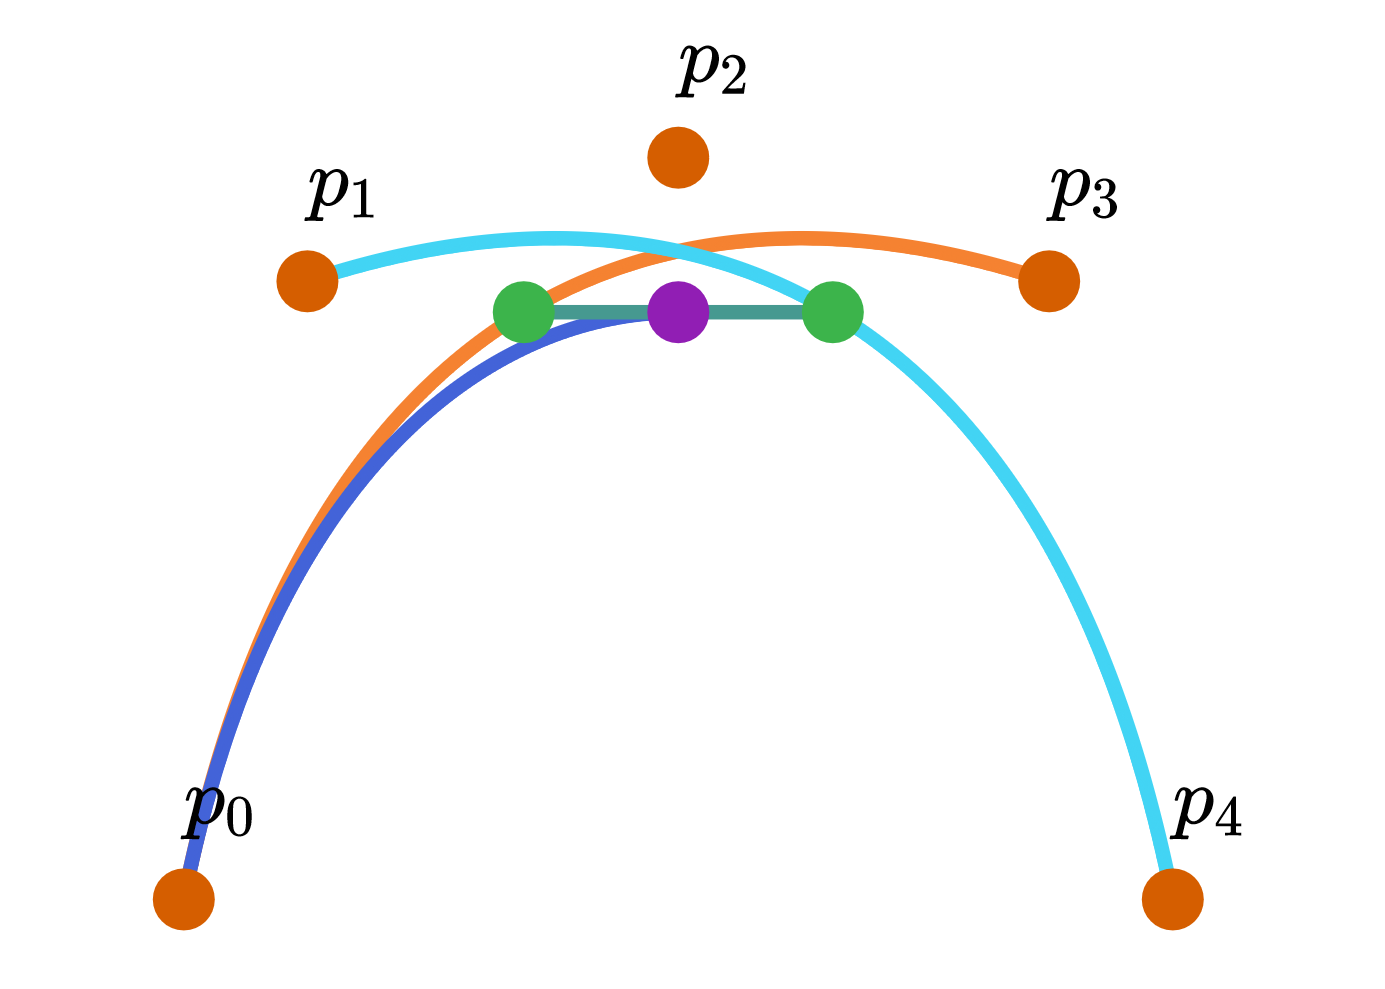
\includegraphics[width = \groupimagewidth]{images/decasteljau-2-t-05}}\\
        \subfloat[$t=0.75$]{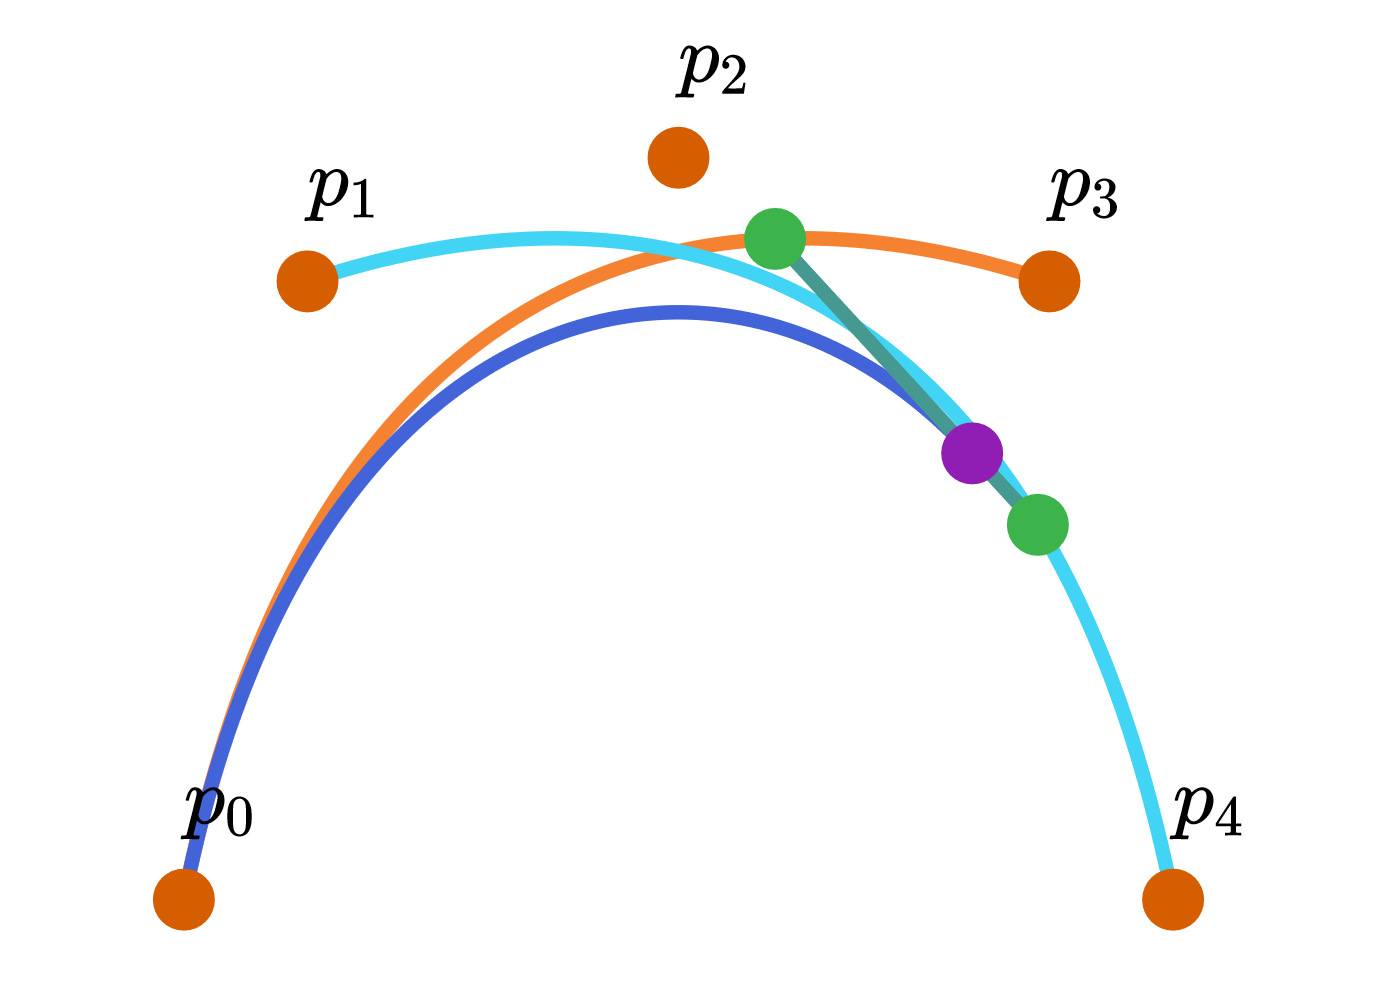
\includegraphics[width = \groupimagewidth]{images/decasteljau-2-t-075}}
        \qquad
        \subfloat[$t=1$]{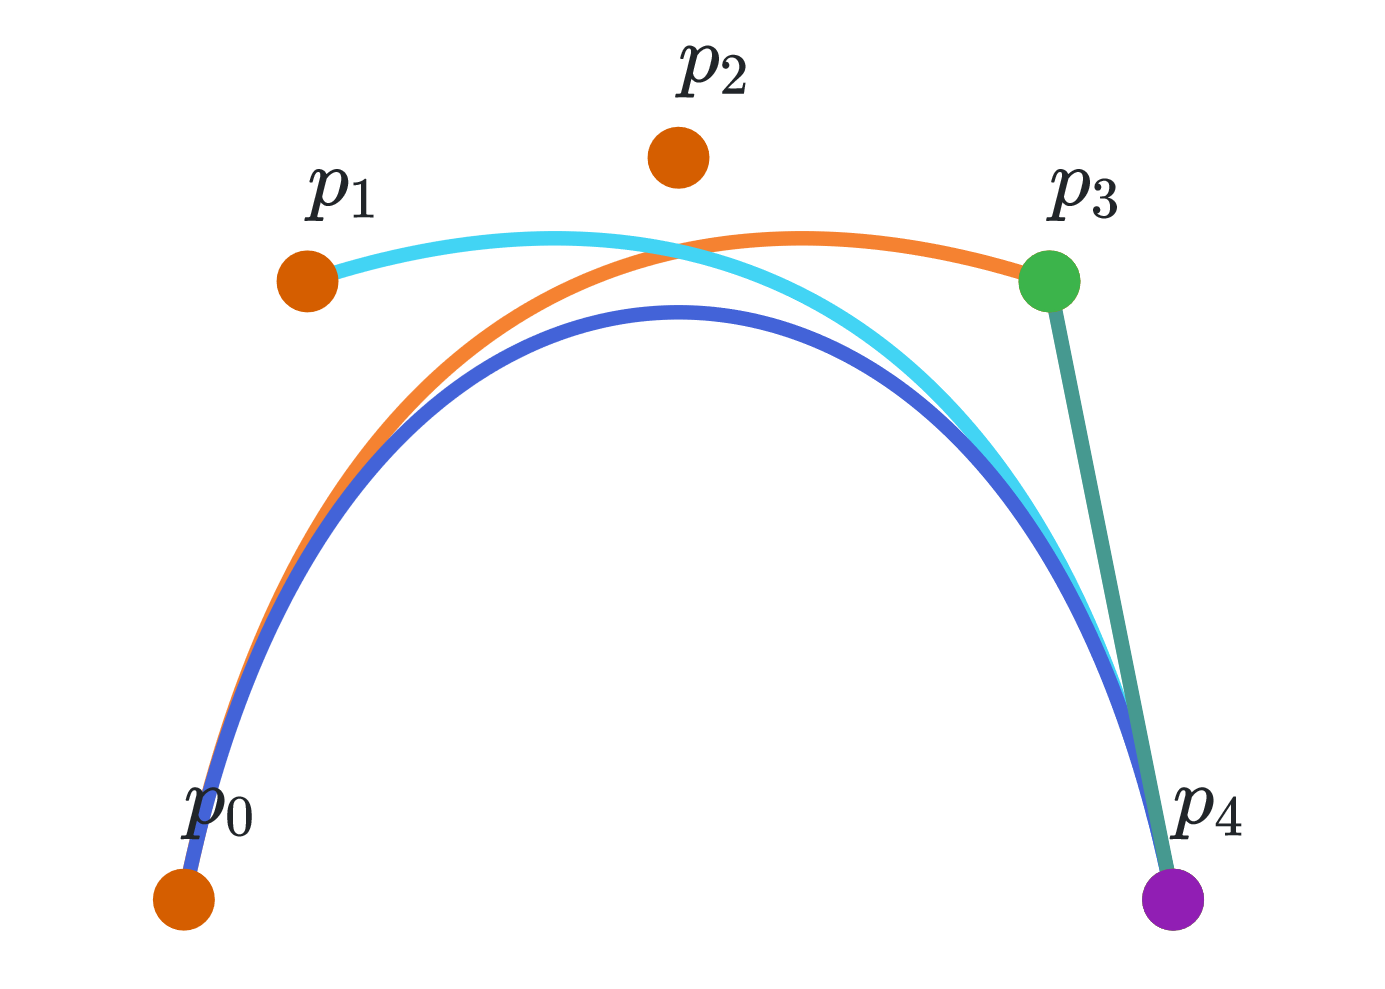
\includegraphics[width = \groupimagewidth]{images/decasteljau-2-t-1}}
        \caption{Izračun točke Bézierjeve krivulje.}
        \label{fig:decasteljau-2}
    \end{figure}

    Označimo sedaj $\p_{i}^r(t) = \bigbbt_{[\p_i,\p_{i+1},\dots,\p_{i+r}]}$.
    Velja torej $\p_{i}^0(t)=\p_i$ in  $\p_{0}^n(t)=\bigbbt_{[\p_0,\p_1,\dots,\p_n]}$.
    Iz izreka~\ref{izrek:decastelaju-rekurzija} sledi, da lahko točke Bézierjeve krivulje $\bigbbt_{[\p_0,\p_1,\dots,\p_n]}$ računamo s pomočjo \textit{de Casteljaujeve sheme}, ki jo lahko vidimo na sliki~\ref{fig:decasteljau-scheme}.
    V shemi diagonalne puščice ponazarjajo množenje točke z vrednostjo $t$, vertikalne pa z vrednostjo $1-t$.
    V vrhu puščic dobljene vrednosti seštejemo.
    \begin{figure}[H]
        \label{fig:decasteljau-scheme}
        \begin{tabular}{ c c c c c c c c c c c}
            $\p_{0}^n(t)$     &            &                   &            &               &            &          &            &                 &            &               \\
            $\uparrow$        & $\nwarrow$ &                   &            &               &            &          &            &                 &            &               \\
            $\p_{0}^{n-1}(t)$ &            & $\p_{1}^{n-1}(t)$ &            &               &            &          &            &                 &            &               \\
            $\vdots$          & $\vdots$   & $\vdots$          & $\vdots$   & $\vdots$      &            & $\vdots$ &            &                 &            &               \\
            $\uparrow$        & $\nwarrow$ & $\uparrow$        & $\nwarrow$ & $\uparrow$    & $\nwarrow$ & $\cdots$ & $\nwarrow$ &                 &            &               \\
            $\p_{0}^1(t)$     &            & $\p_{1}^1(t)$     &            & $\p_{2}^1(t)$ &            & $\cdots$ &            & $\p_{n-1}^1(t)$ &            &               \\
            $\uparrow$        & $\nwarrow$ & $\uparrow$        & $\nwarrow$ & $\uparrow$    & $\nwarrow$ & $\cdots$ & $\nwarrow$ & $\uparrow$      & $\nwarrow$     &\\
            $\p_{0}^0(t)$     &            & $\p_{1}^0(t)$     &            & $\p_{2}^0(t)$ &            & $\cdots$ &            & $\p_{n-1}^0(t)$ &            & $\p_{n}^0(t)$
        \end{tabular}
        \caption{De Casteljaujeva shema.}
    \end{figure}
    \noindent Izračun točke Bézierjeve krivulje pri poljubnem parametru $t$ lahko sedaj podamo v obliki \textit{de Casteljaujevega algoritma}~\ref{alg:decasteljau}.
    \begin{algorithm}[H]
        \caption{De Casteljaujev algoritem}
        \label{alg:decasteljau}
        \begin{algorithmic}
            \State $\p \gets \p_0,\p_1,\dots,\p_n$
            \State $t \gets t$
            \For{$i = 0,1,\dots n$}
                \State $\p_i^0(t)=\p_i$
            \EndFor
            \For{$r = 1,2,\dots n$}
                \For{$i=0,1,\dots,n-r$}
                    \State $\p_i^r(t)=(1-t)\p_i^{r-1}(t)+t\p_{i+1}^{r-1}(t)$
                \EndFor
            \EndFor
            \State \Return $\p_0^n(t)$
        \end{algorithmic}
    \end{algorithm}
    \noindent De Casteljaujev algoritem ima tudi geometrijski pomen.
    Pri stopnji $n=1$ se prevede na interpolacijo dveh točk, kar lahko vidimo na sliki~\ref{fig:dec-alg-n1}.
    Pri višjih stopnjah $n$ pa algoritem predstavlja zaporedno interpolacijo točk, saj v njem za vsak nivo $r=1,2,\ldots,n$ interpoliramo sosednje točke prejšnjega nivoja.
    Slednje lahko vidimo na slikama~\ref{fig:dec-alg-n2} in~\ref{fig:dec-alg-n3}.
    \begin{figure}[h!]
        \captionsetup[subfigure]{labelformat=empty}
        \centering
        \subfloat[$t=0.25$]{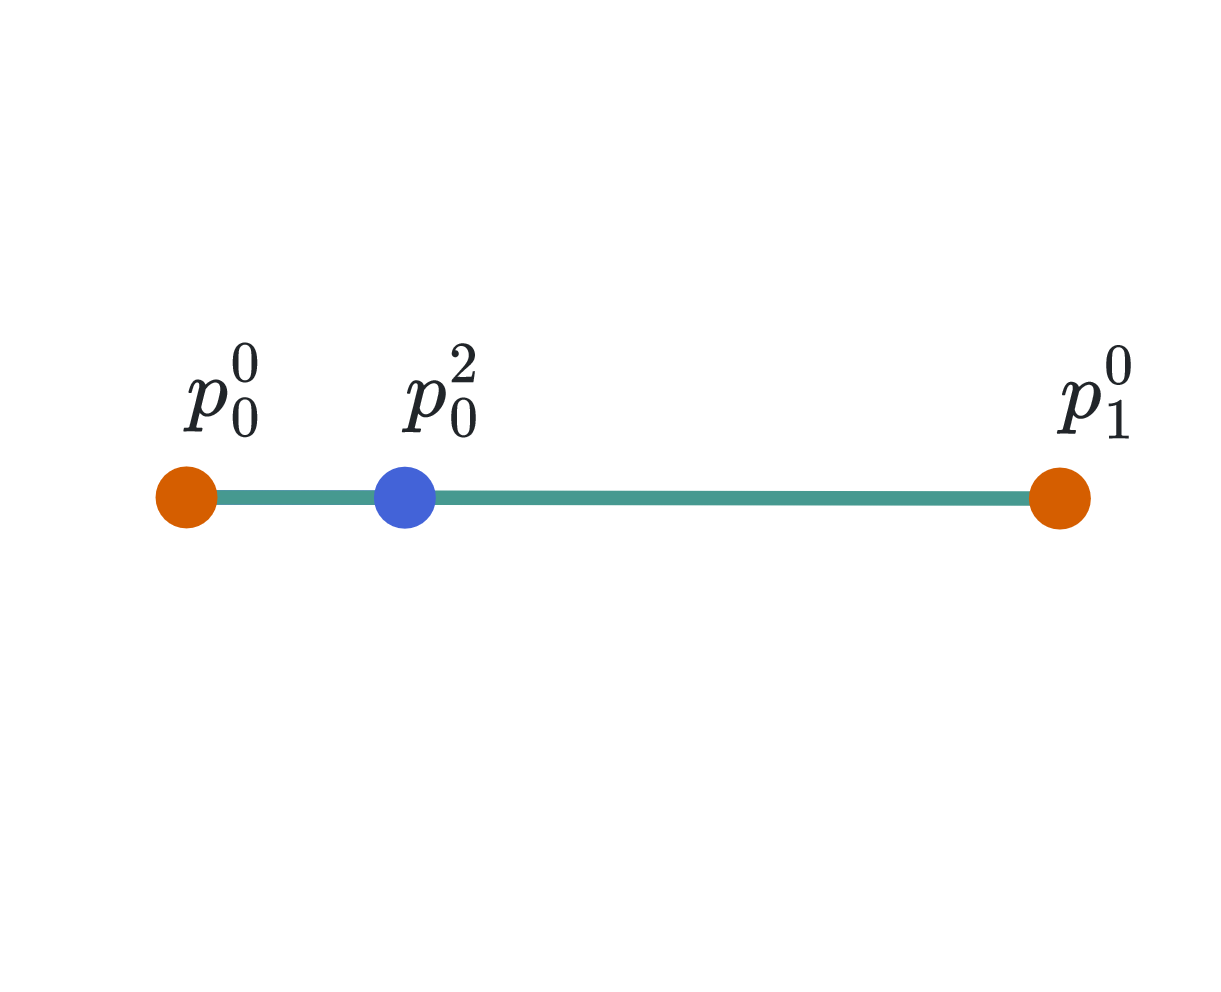
\includegraphics[width = \groupimagewidth]{images/decasteljau-n-1-t-025}}
        \qquad
        \subfloat[$t=0.5$]{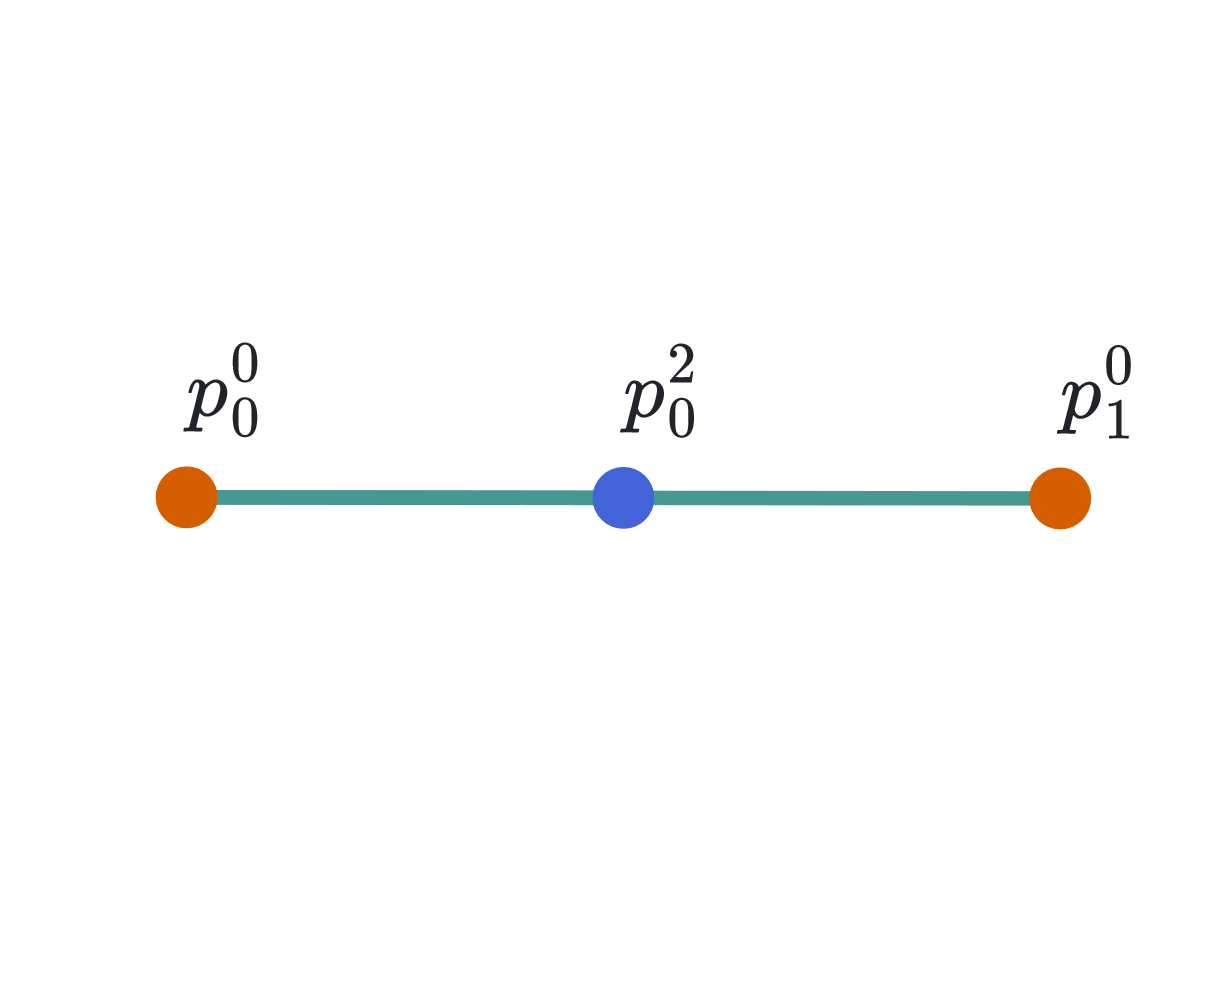
\includegraphics[width = \groupimagewidth]{images/decasteljau-n-1-t-05}}
        \\
        \subfloat[$t=0.75$]{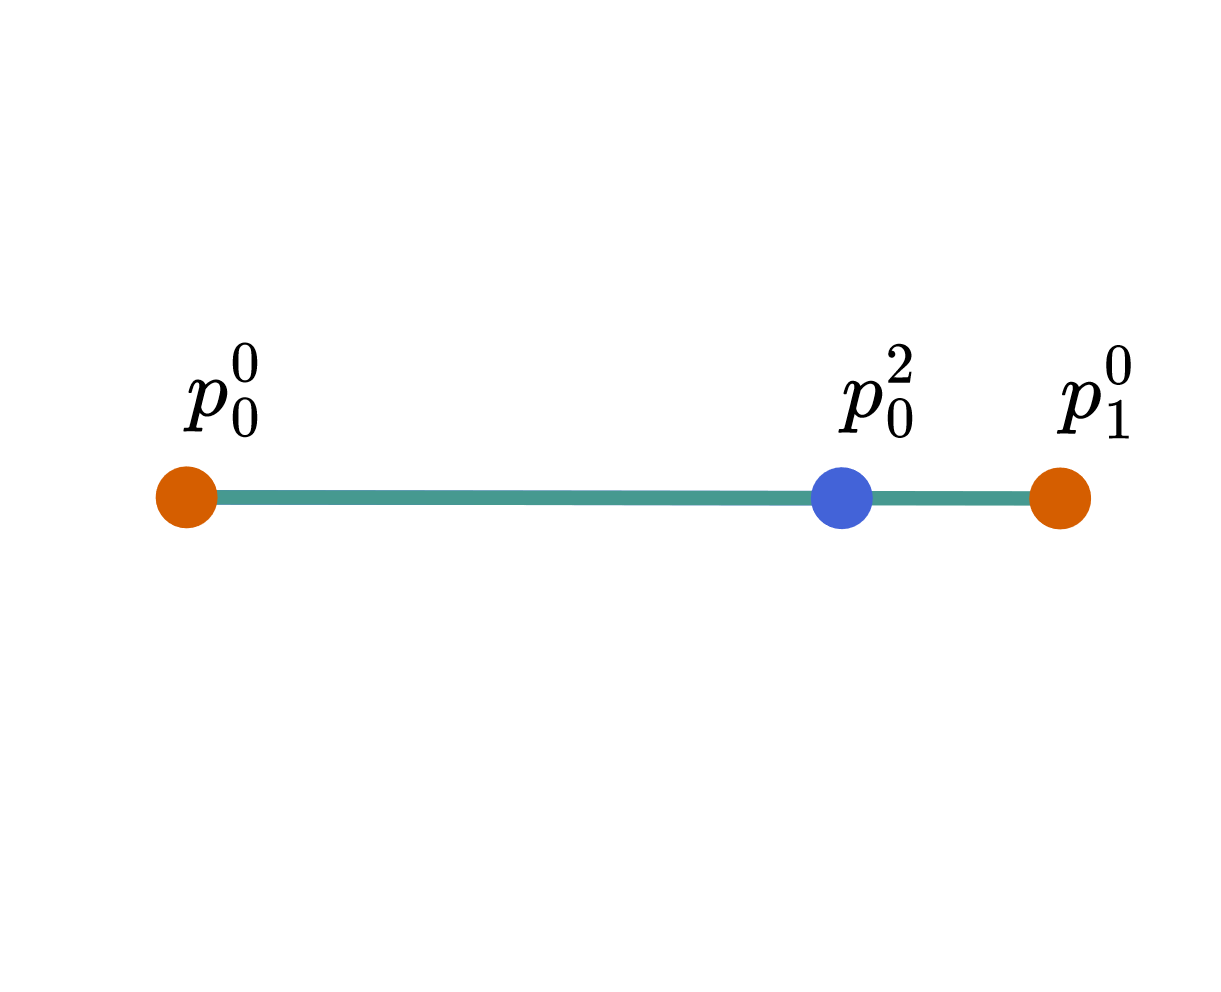
\includegraphics[width = \groupimagewidth]{images/decasteljau-n-1-t-075}}
        \qquad
        \subfloat[$t=1$]{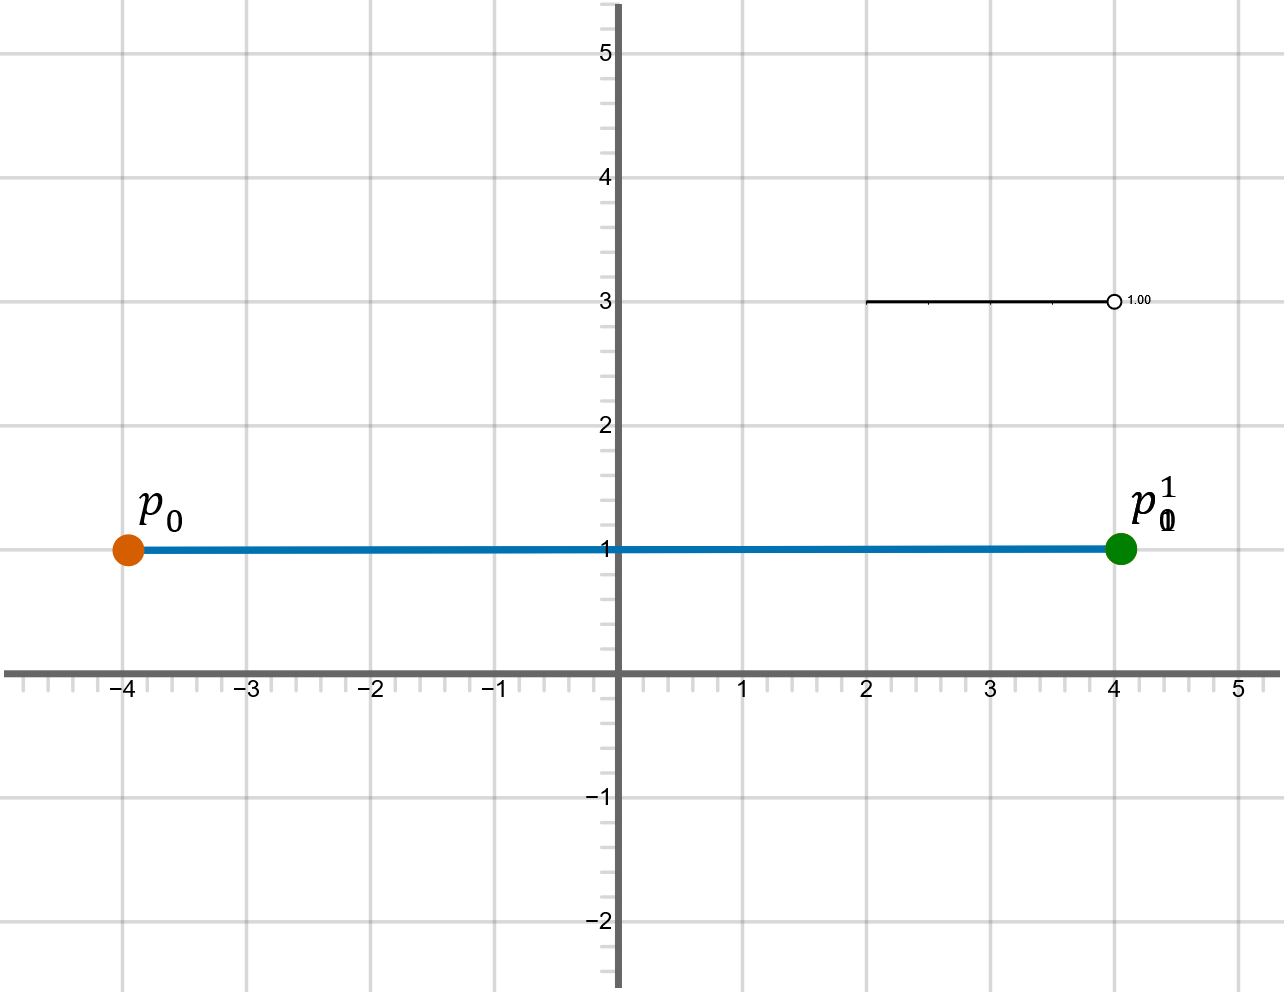
\includegraphics[width = \groupimagewidth]{images/decasteljau-n-1-t-1}}
        \caption{De Casteljaujev algoritem za $n=1$.}
        \label{fig:dec-alg-n1}
    \end{figure}
    \begin{figure}[h!]
        \captionsetup[subfigure]{labelformat=empty}
        \centering
        \subfloat[$t=0.25$]{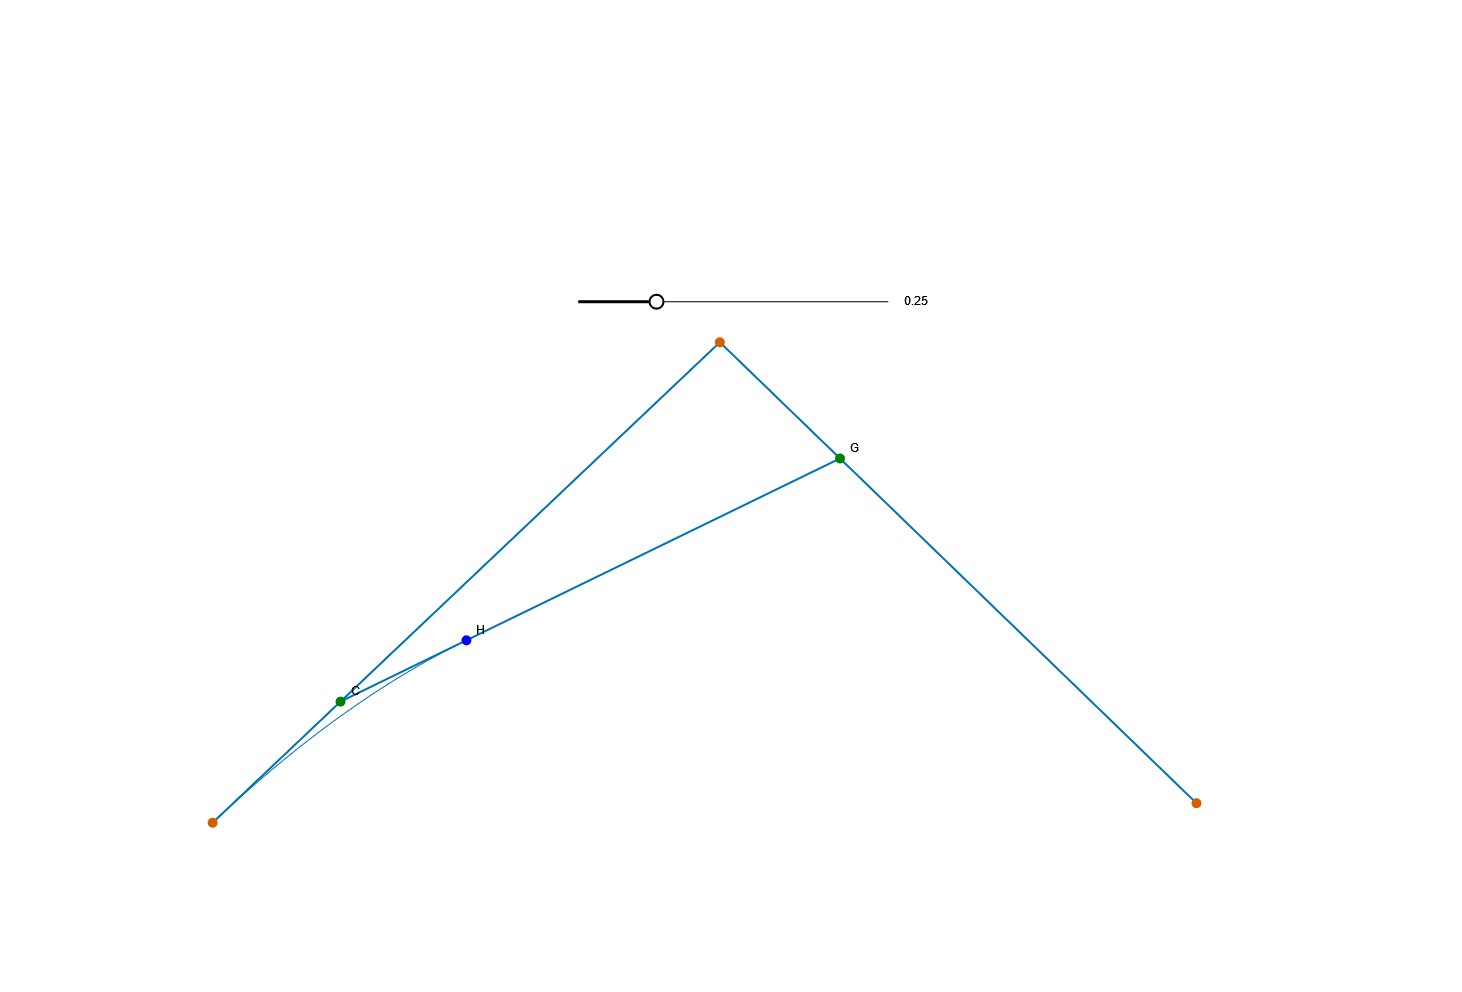
\includegraphics[width = \groupimagewidth]{images/decasteljau-n-2-t-025}}
        \qquad
        \subfloat[$t=0.5$]{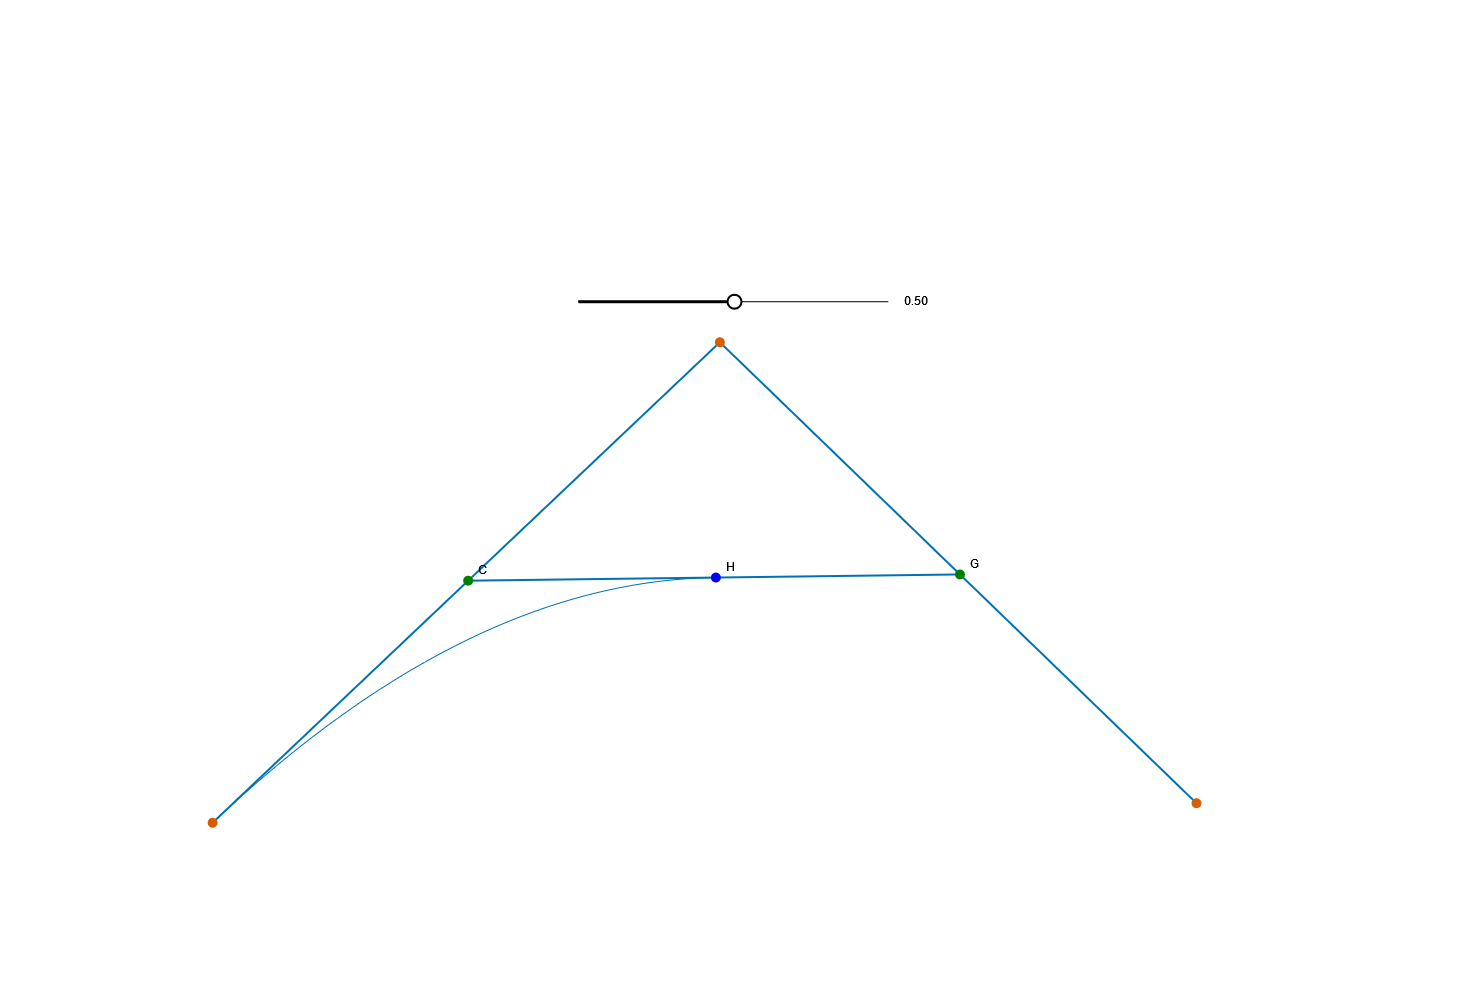
\includegraphics[width = \groupimagewidth]{images/decasteljau-n-2-t-05}}
        \\
        \subfloat[$t=0.75$]{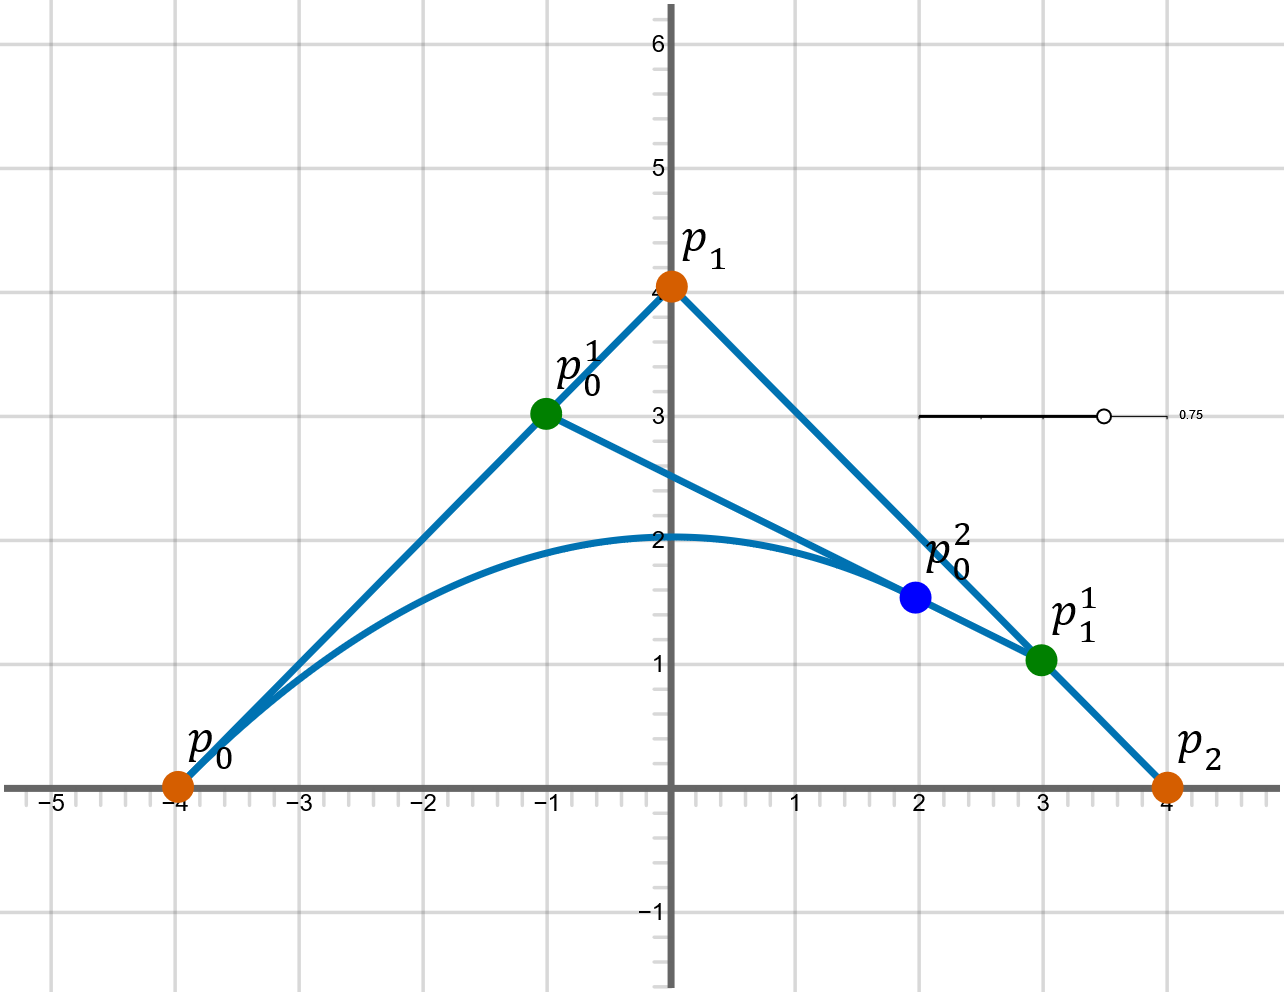
\includegraphics[width = \groupimagewidth]{images/decasteljau-n-2-t-075}}
        \qquad
        \subfloat[$t=1$]{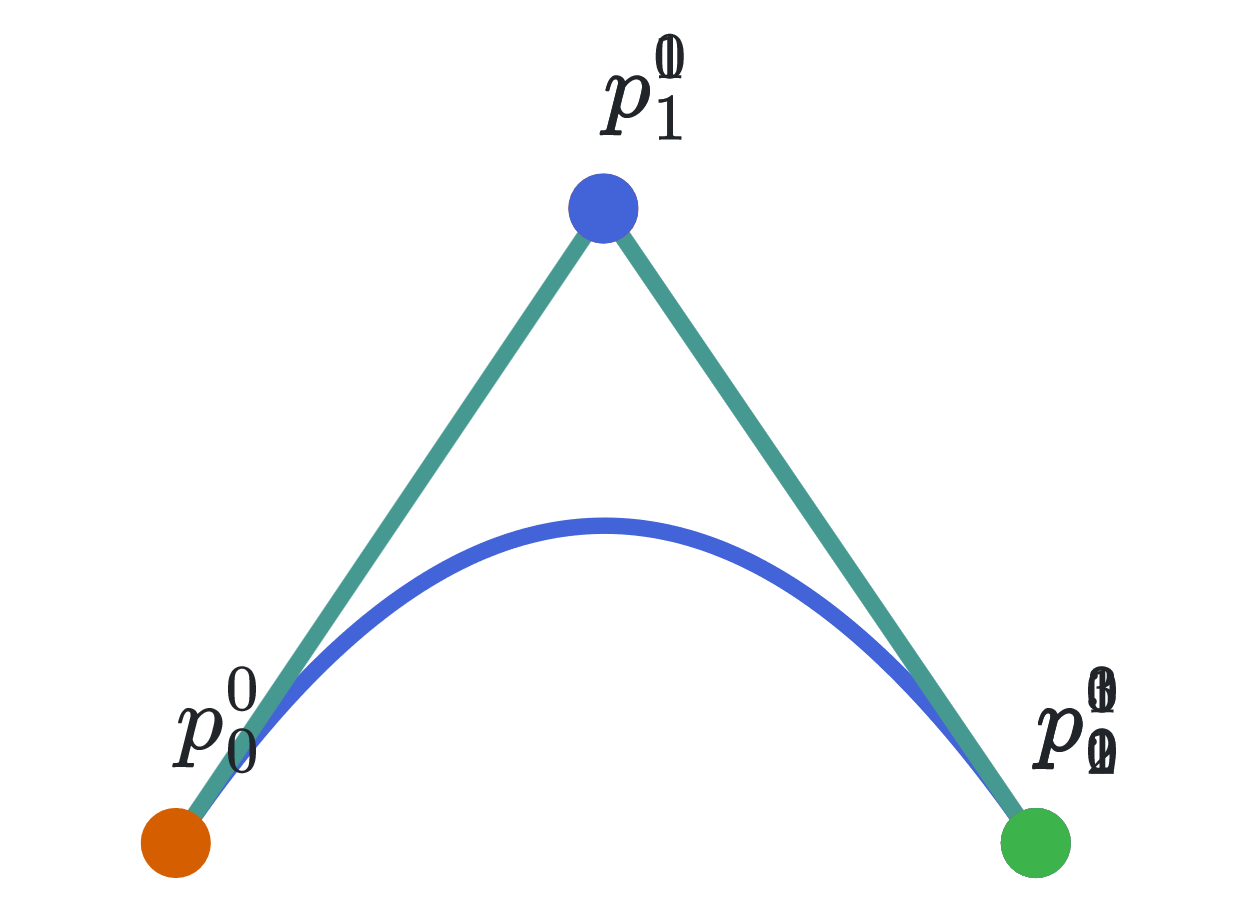
\includegraphics[width = \groupimagewidth]{images/decasteljau-n-2-t-1}}
        \caption{De Casteljaujev algoritem za $n=2$.}
        \label{fig:dec-alg-n2}
    \end{figure}
    \begin{figure}[h!]
        \captionsetup[subfigure]{labelformat=empty}
        \centering
        \subfloat[$t=0.25$]{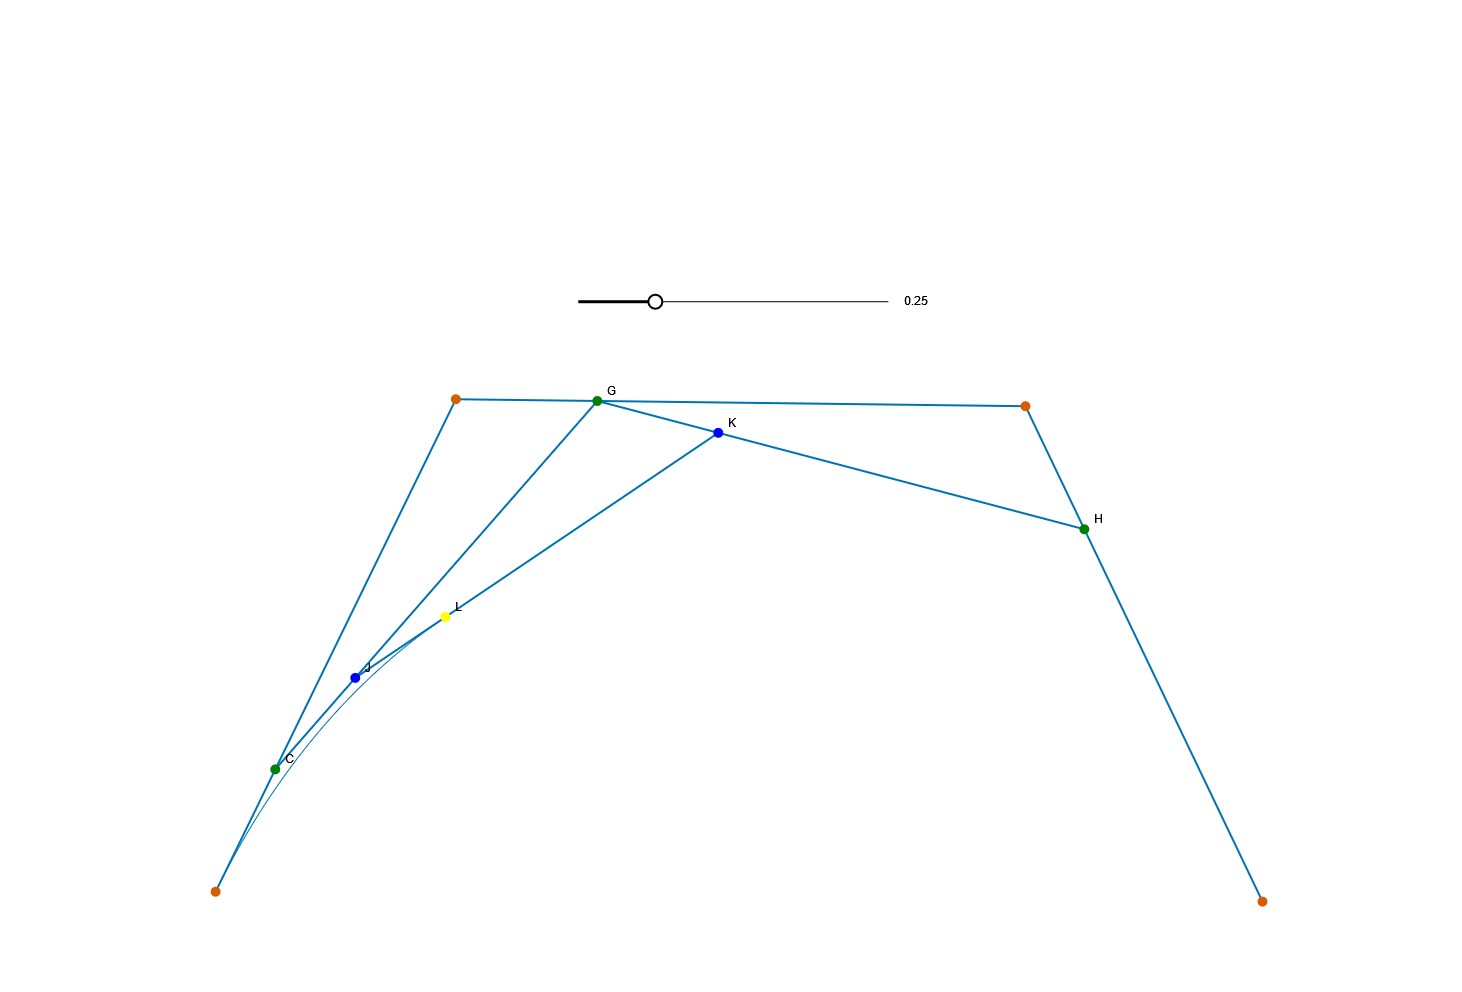
\includegraphics[width = \groupimagewidth]{images/decasteljau-n-3-t-025}}
        \qquad
        \subfloat[$t=0.5$]{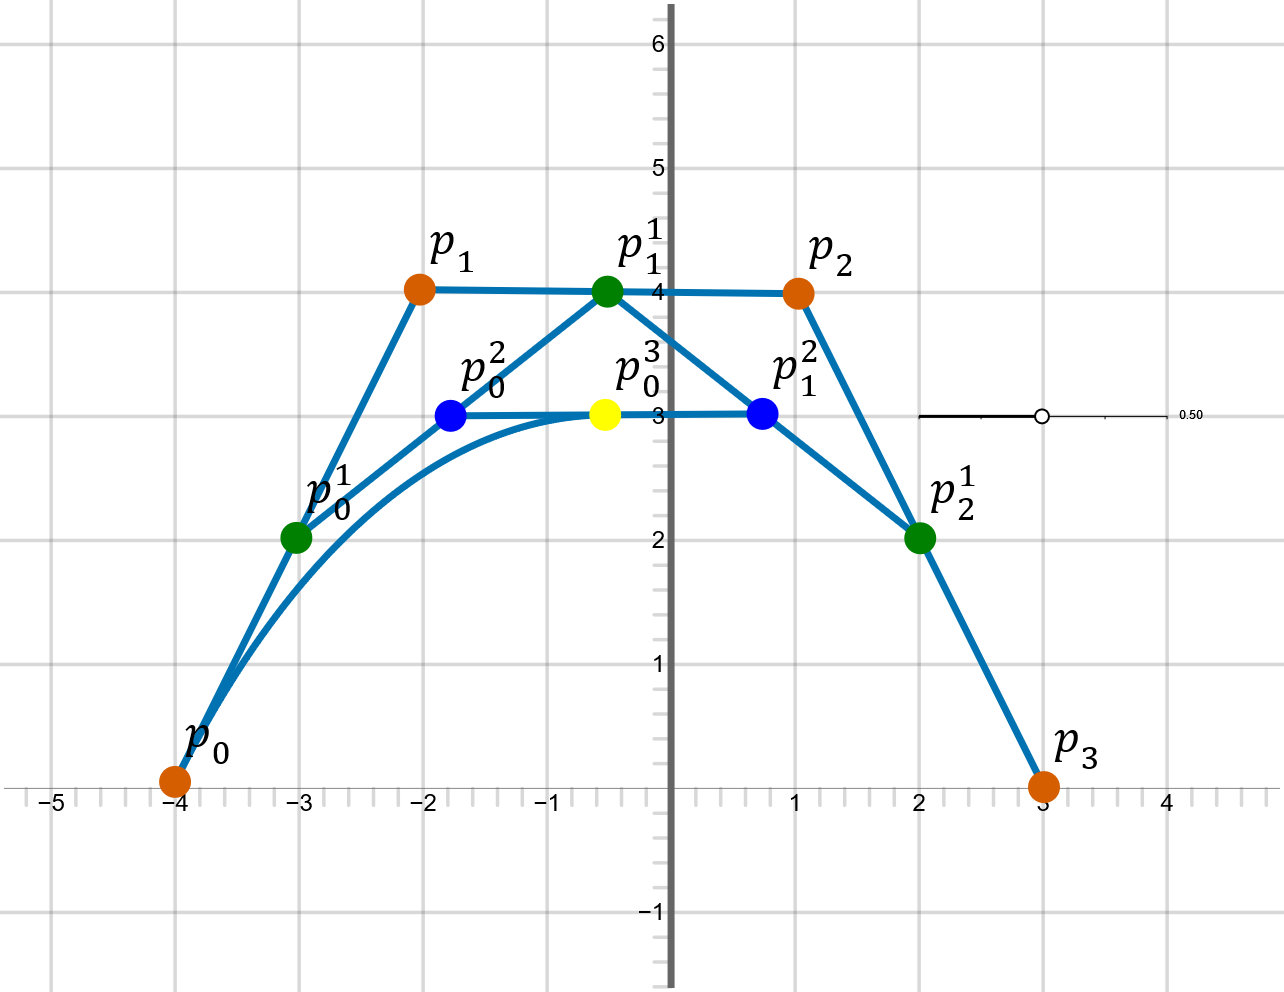
\includegraphics[width = \groupimagewidth]{images/decasteljau-n-3-t-05}}
        \\
        \subfloat[$t=0.75$]{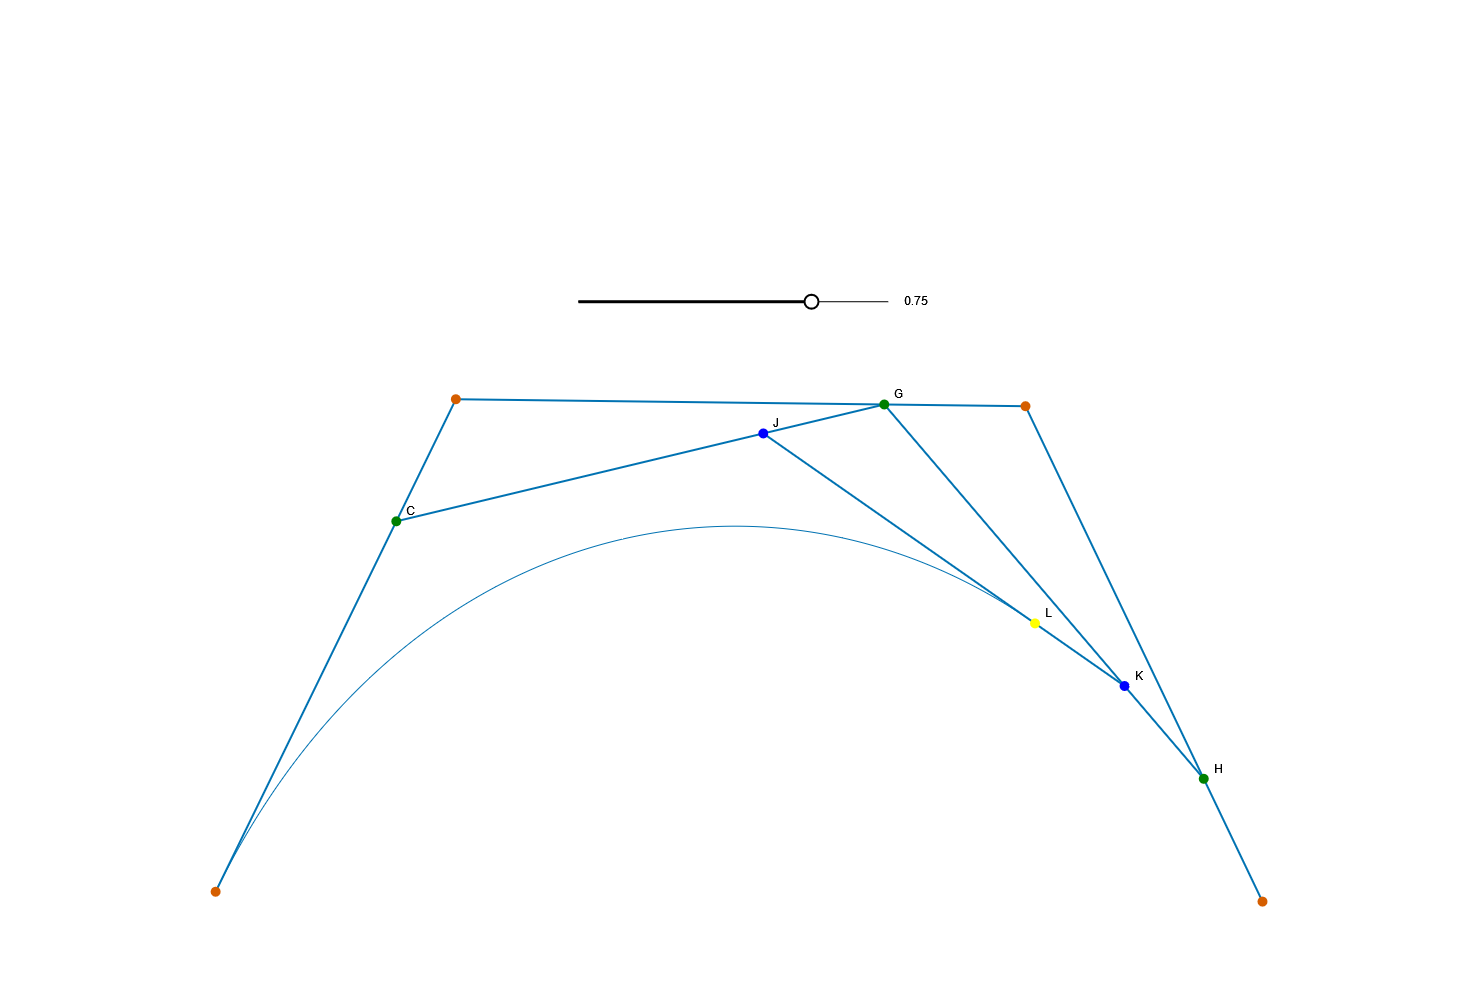
\includegraphics[width = \groupimagewidth]{images/decasteljau-n-3-t-075}}
        \qquad
        \subfloat[$t=1$]{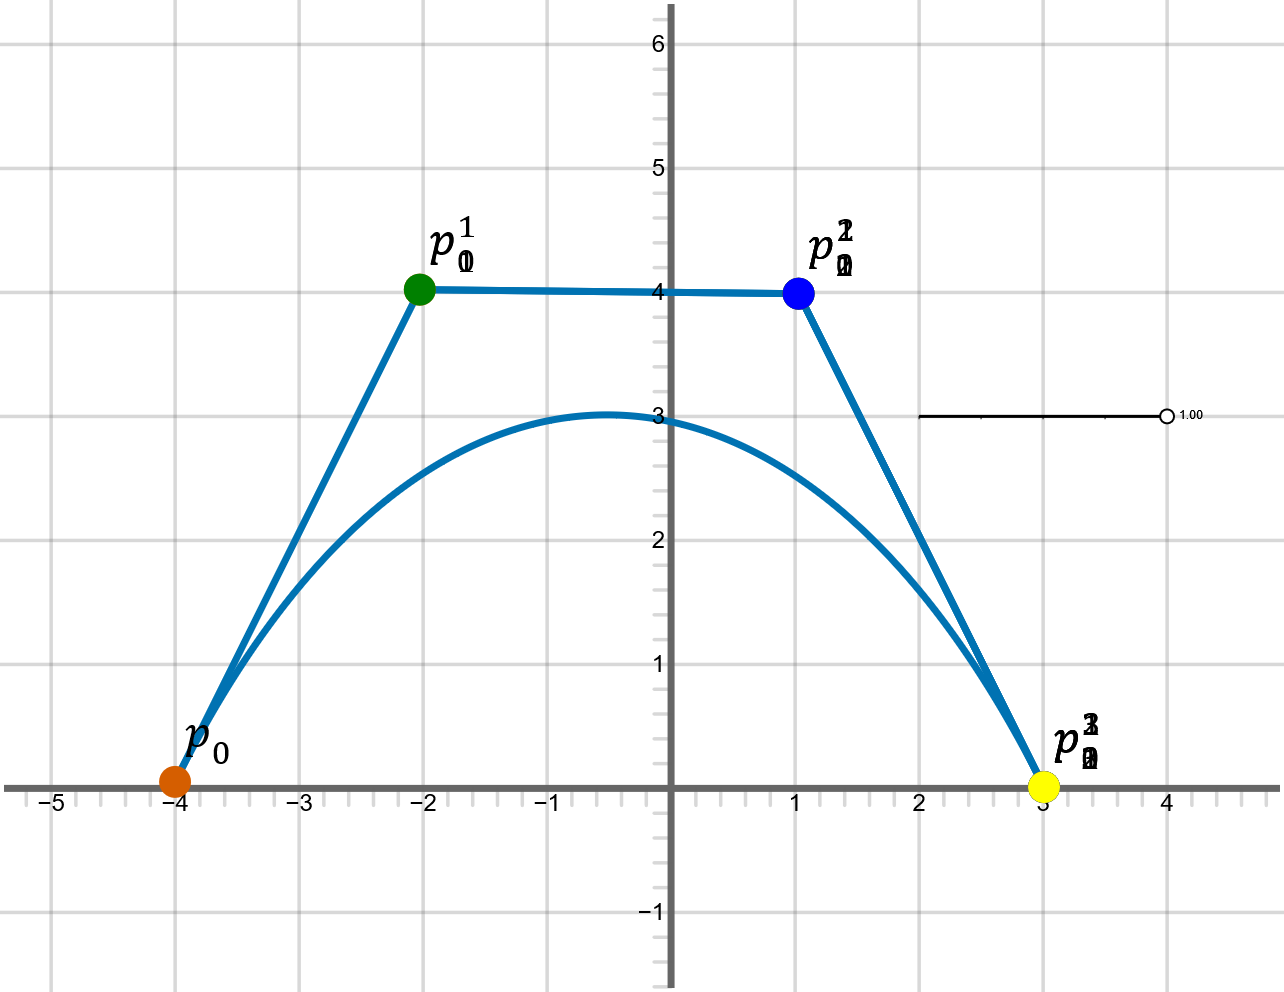
\includegraphics[width = \groupimagewidth]{images/decasteljau-n-3-t-1}}
        \caption{De Casteljaujev algoritem za $n=3$.}
        \label{fig:dec-alg-n3}
    \end{figure}
%    \begin{figure}[h!]
%        \captionsetup[subfigure]{labelformat=empty}
%        \centering
%        \subfloat[$t=0.25$]{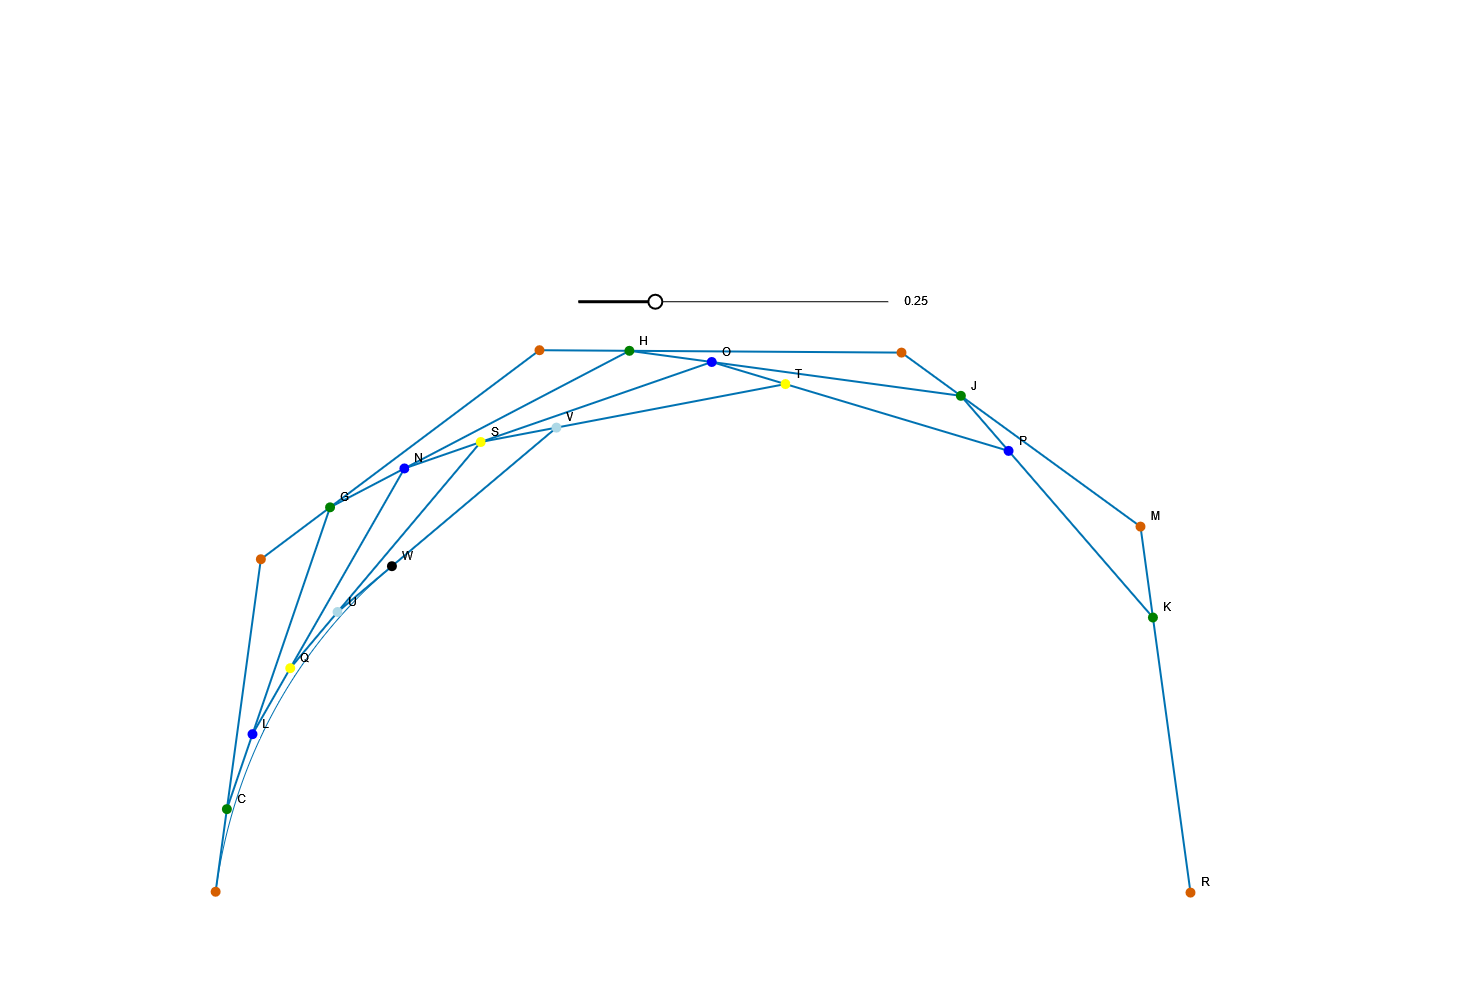
\includegraphics[width = \groupimagewidth]{images/decasteljau-n-5-t-025}}
%        \qquad
%        \subfloat[$t=0.5$]{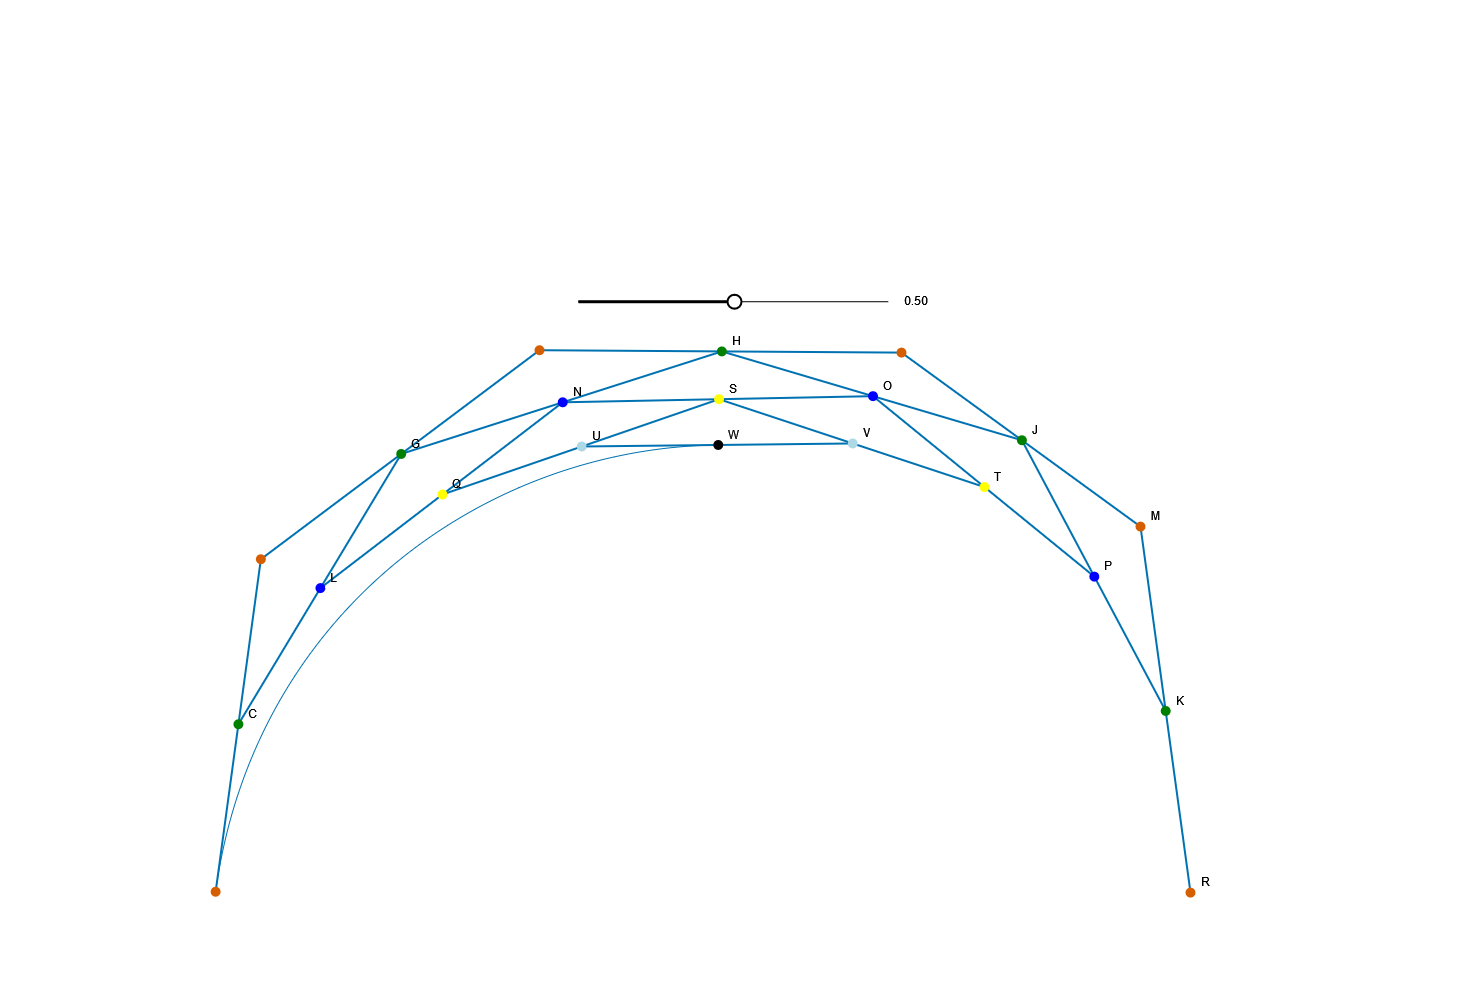
\includegraphics[width = \groupimagewidth]{images/decasteljau-n-5-t-05}}
%        \qquad
%        \subfloat[$t=0.75$]{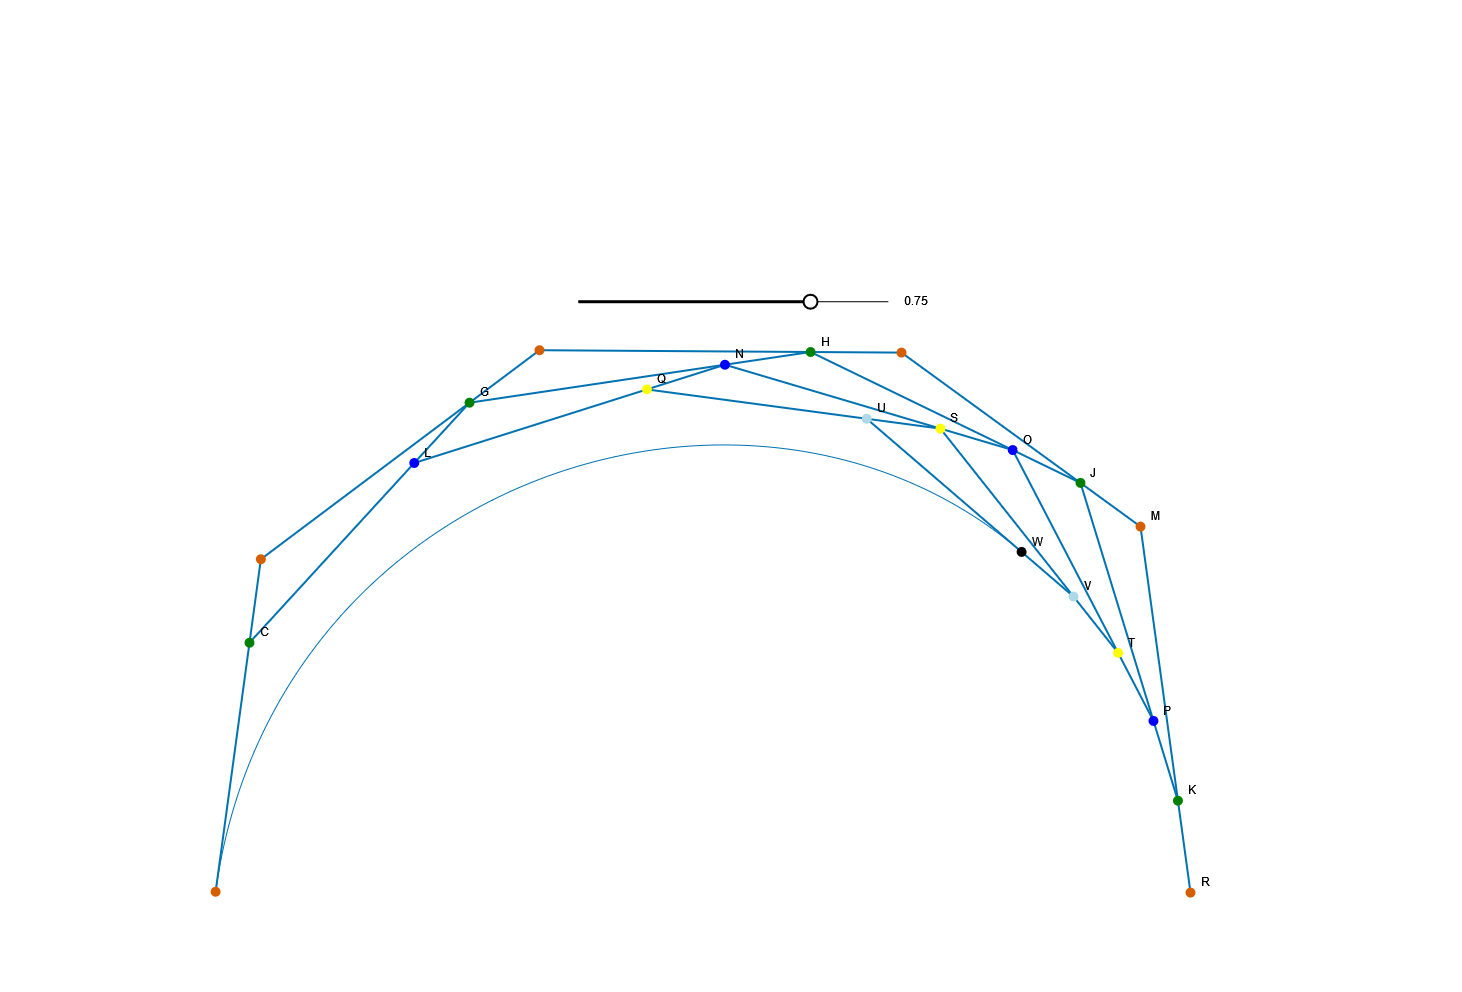
\includegraphics[width = \groupimagewidth]{images/decasteljau-n-5-t-075}}
%        \qquad
%        \subfloat[$t=1$]{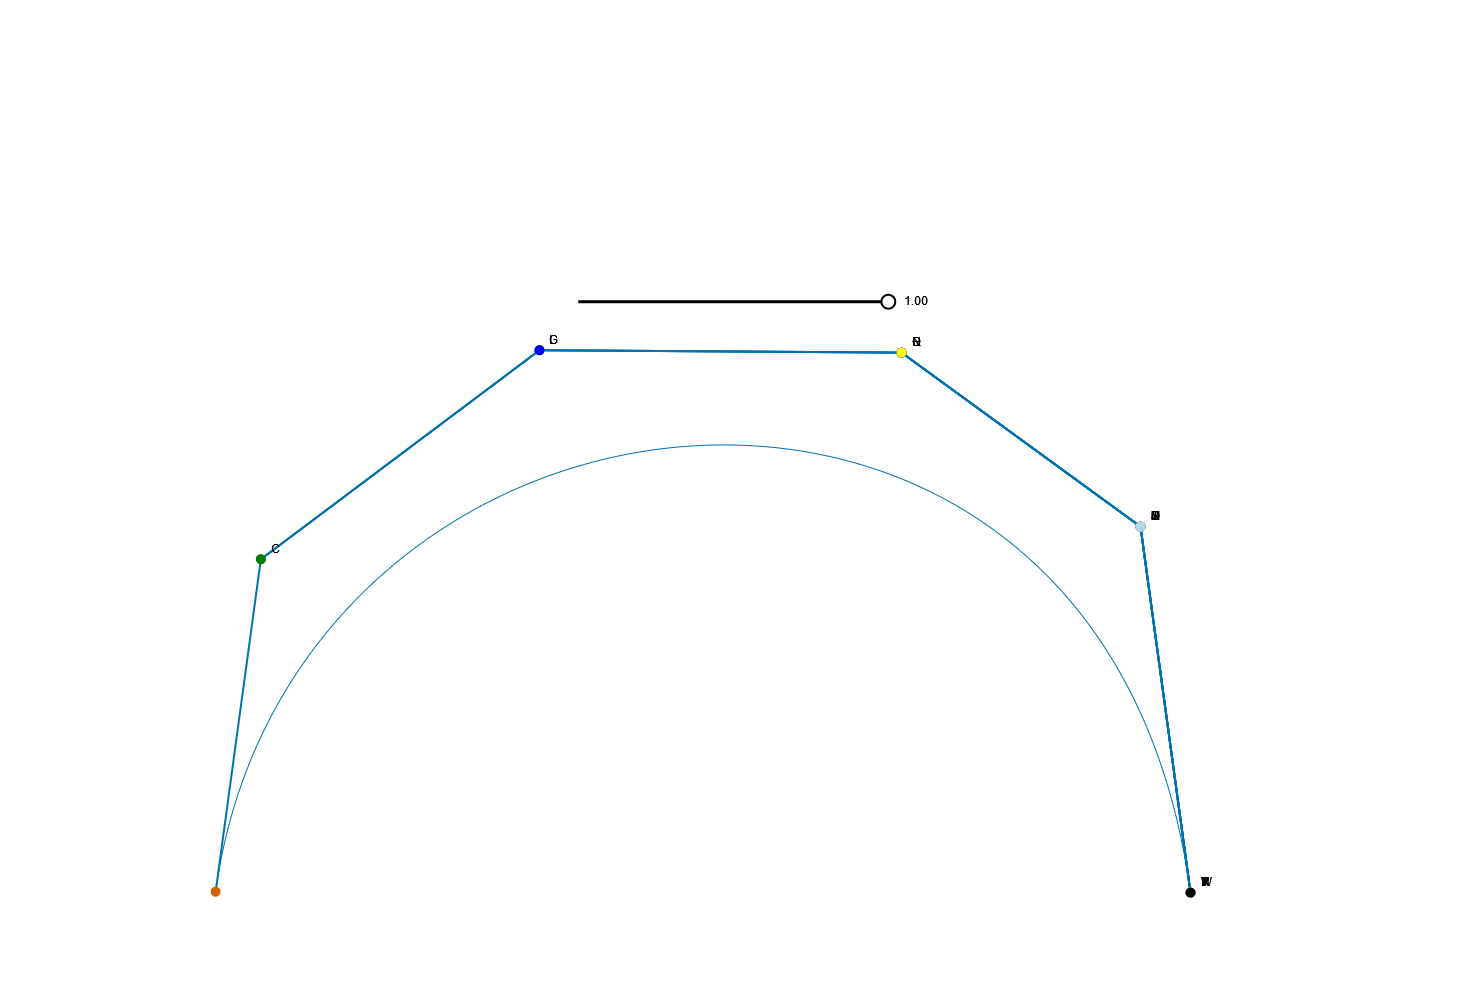
\includegraphics[width = \groupimagewidth]{images/decasteljau-n-5-t-1}}
%        \caption{De Casteljaujev algoritem za $n=5$}
%        \label{fig:dec-alg-n5}
%    \end{figure}

    \subsection{Subdivizija}
    V CAGD in CAD sistemih se mnogokrat zgodi, da uporabnik želi ohraniti le en del Bézierjeve krivulje.
    Naj bo to tisti del krivulje, ki ga dobimo tako, da za prvotno krivuljo parameter $t$ omejimo na interval $[0,t_0]$, za neko pozitivno realno število $t_0<1$.
    Ta del krivulje označimo z $B_{t_0-}$.
    Izkaže se, da lahko krivuljo $B_{t_0-}$ podamo kot Bézierjevo krivuljo s kontrolnimi točkami $\p_0^i(t_0)$ za $i=0,1,\ldots,n$, kjer točke $\p_0^i(t_0)$ dobimo iz de Casteljaujeve sheme pri $t=t_0$.
    Podobno se izkaže tudi to, da lahko preostali del krivulje, $B_{t_0+}$, podamo kot Bézierjevo krivuljo s kontrolnimi točkami $\p_i^i(t_0)$,  $i=0,1,\ldots,n$.
    Procesu deljenja krivulje na dva dela pravimo \textit{subdivizija}.
    Radovedni bralci lahko dokaz trditev najdejo v delu~\ref{placeholder}.
    Primer si lahko ogledamo na sliki~\ref{fig:subdivizija}.
    \begin{figure}[h]
        \centering
        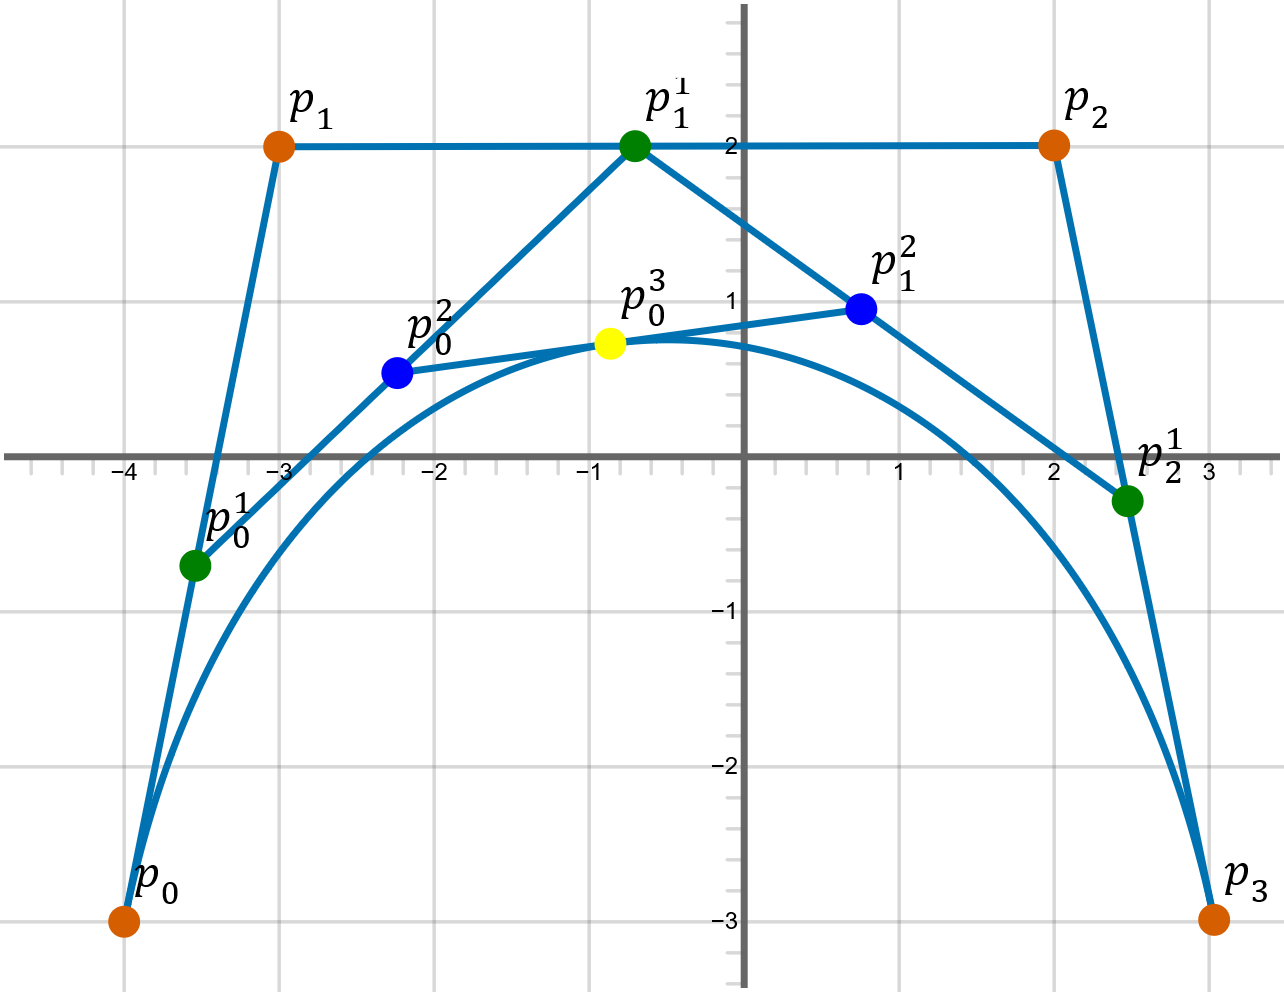
\includegraphics[width=\groupimagewidth]{images/subdivizija}
        \qquad
        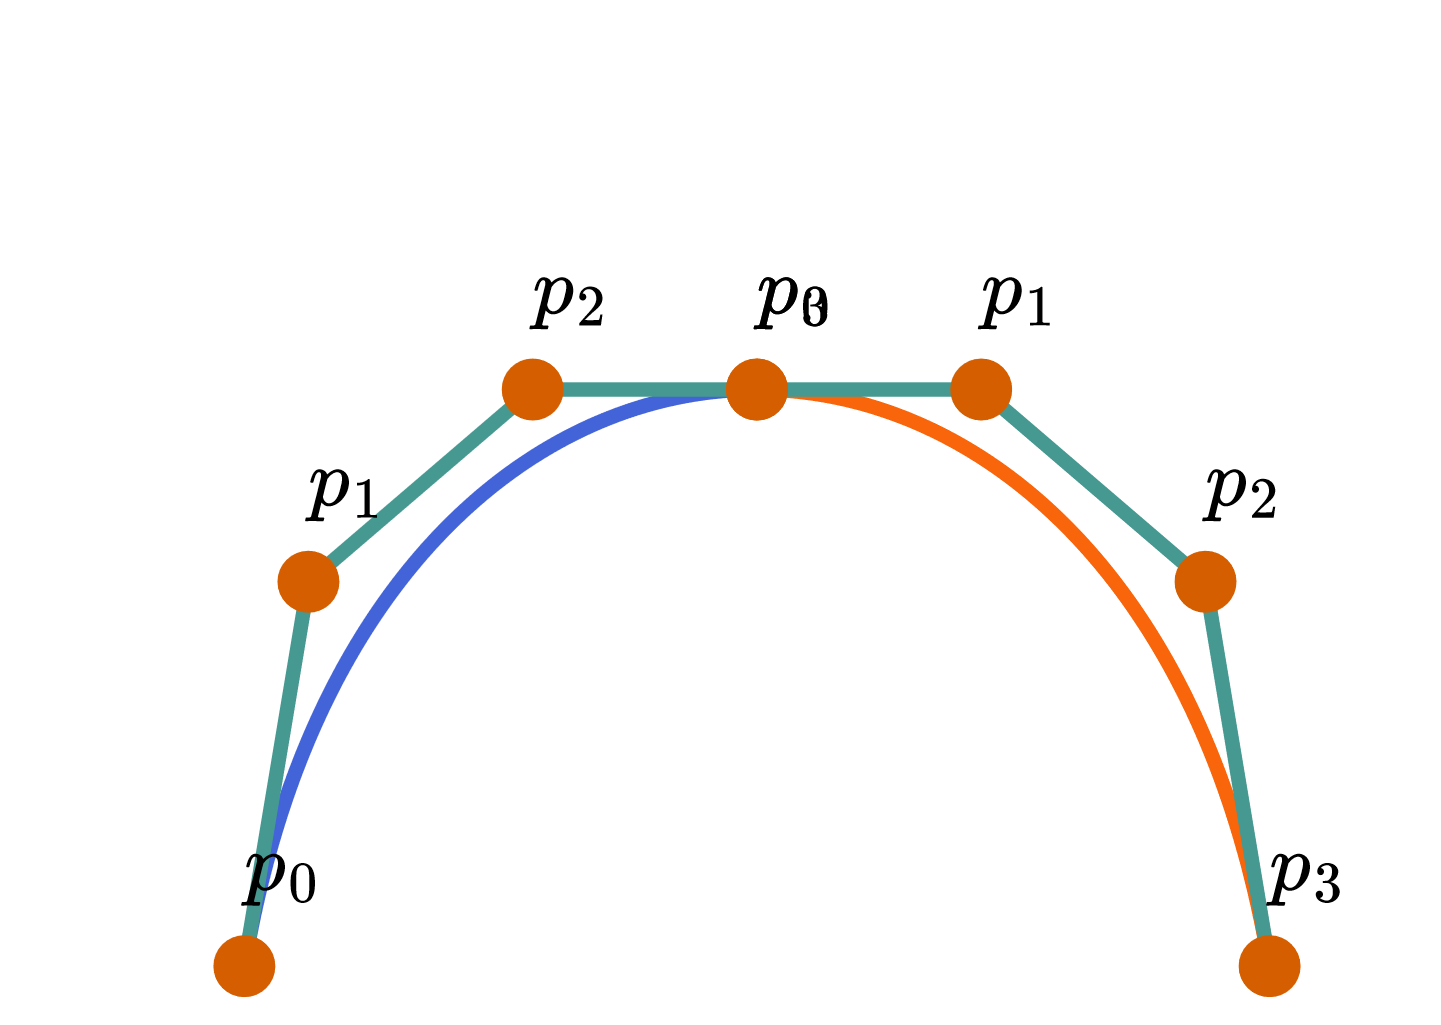
\includegraphics[width=\groupimagewidth]{images/subdivision-split}
        \caption{De Casteljaujeva shema pri $t=t_0$ razdeli krivuljo na dva dela, modrega, $B_{t_0-}$, in oranžnega, $B_{t_0+}$. }
        \label{fig:subdivizija}
    \end{figure}

    Če izberemo sedaj $t_0=\frac{1}{2}$ in krivuljo subdiviziramo, dobimo dve krivulji.
    Če subdivizijo nato na dobljenih krivuljah ponavljamo, dobimo po $k$ korakih $2^k$ krivulj.
    Na sliki~\ref{fig:subdivizija-ponavljanje} si lahko ogledamo postopek za prve tri korake.
    Opazimo, da so kontrolni poligoni dobljenih krivulj zmerom bližje krivulji.
    \begin{figure}[h]
        \captionsetup[subfigure]{labelformat=empty}
        \centering
        \subfloat[začetna krivulja]{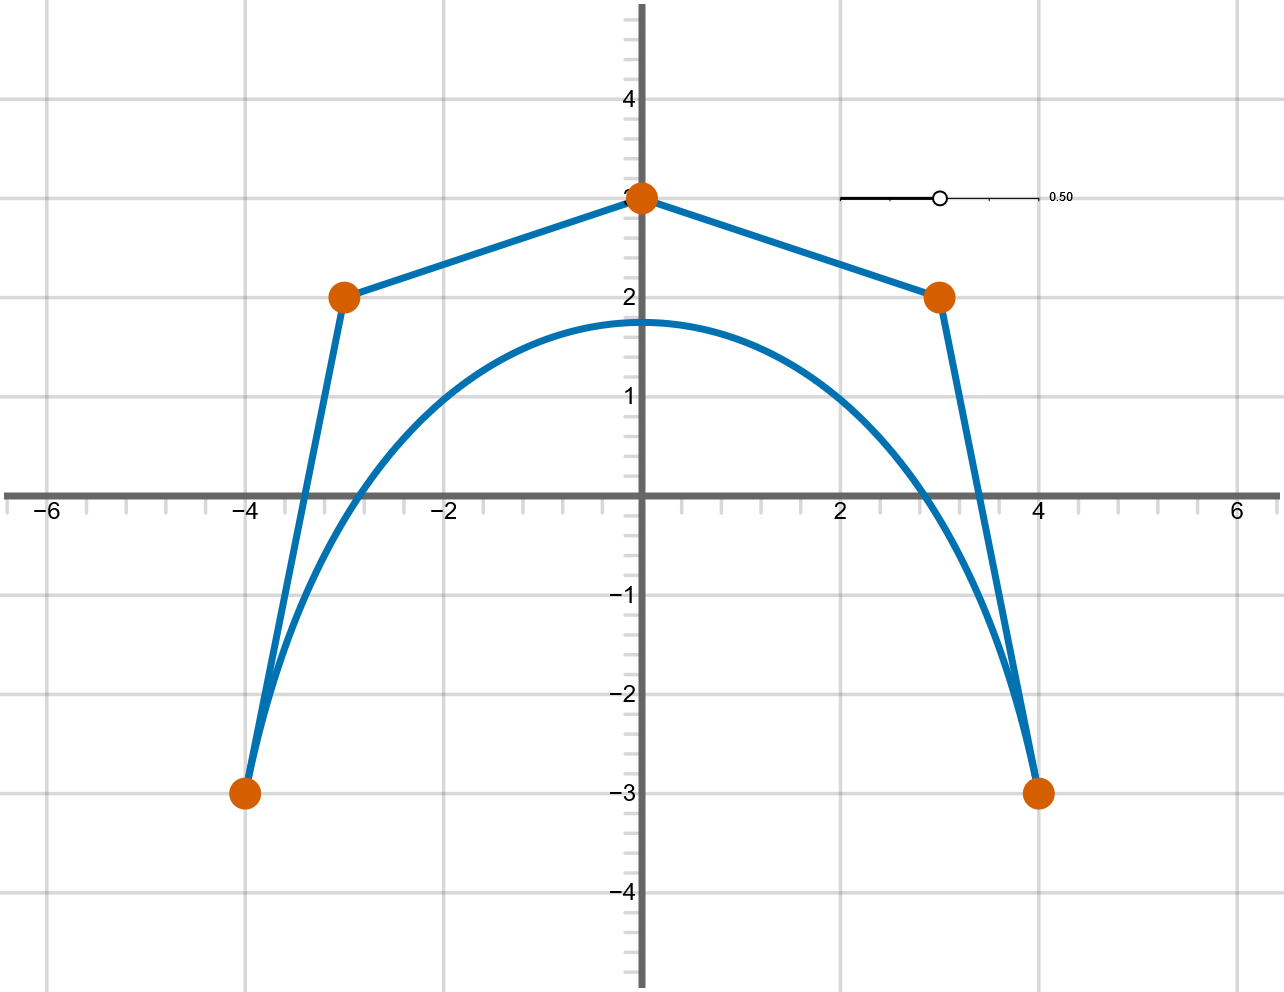
\includegraphics[width = \groupimagewidth]{images/subdivizija-k-0}}
        \qquad
        \subfloat[$2$ krivulji]{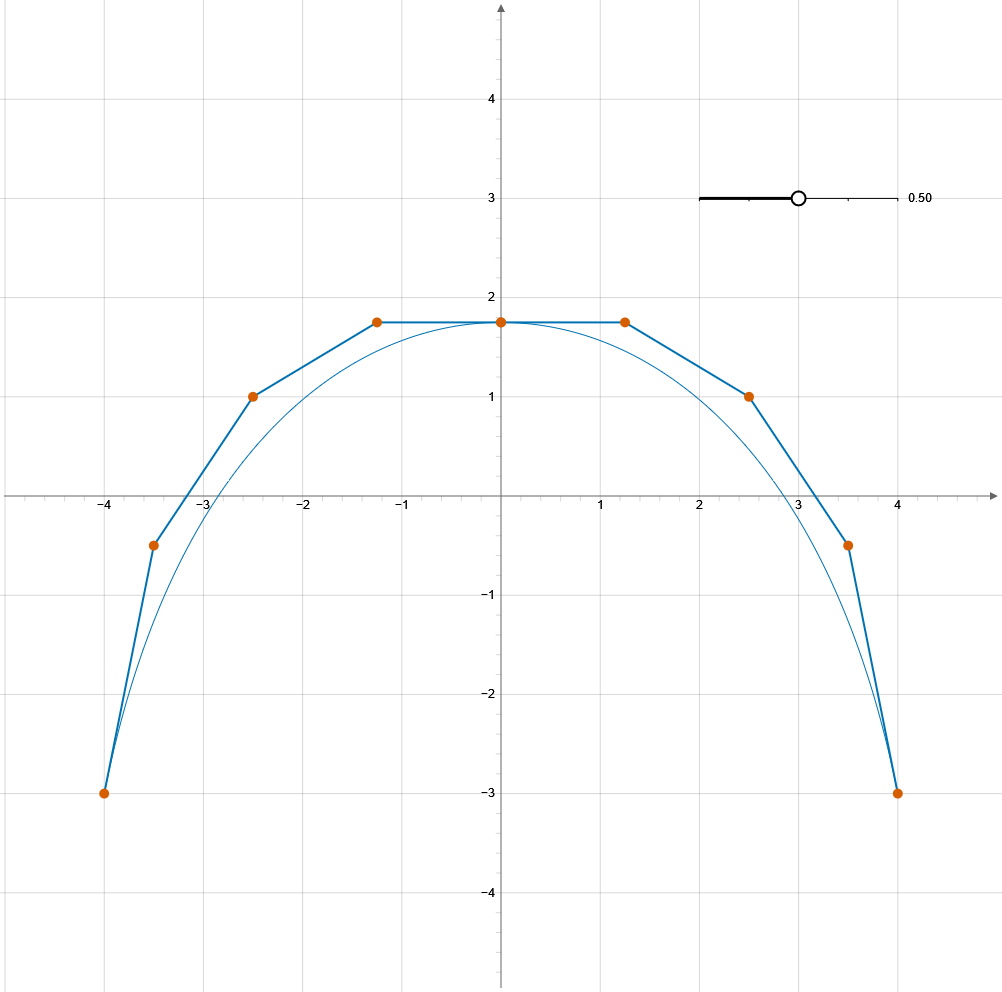
\includegraphics[width = \groupimagewidth]{images/subdivizija-k-1}}

        \subfloat[$4$ krivulje]{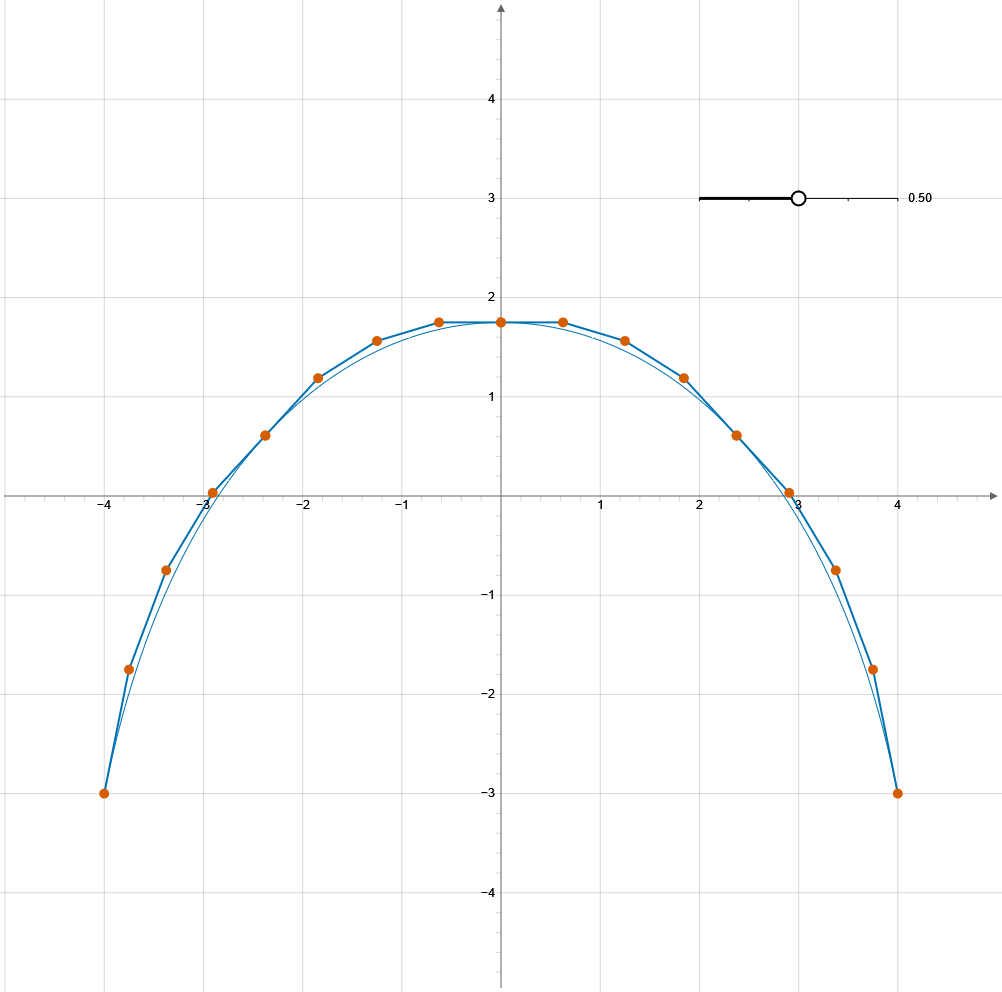
\includegraphics[width = \groupimagewidth]{images/subdivizija-k-2}}
        \qquad
        \subfloat[$8$ krivulj]{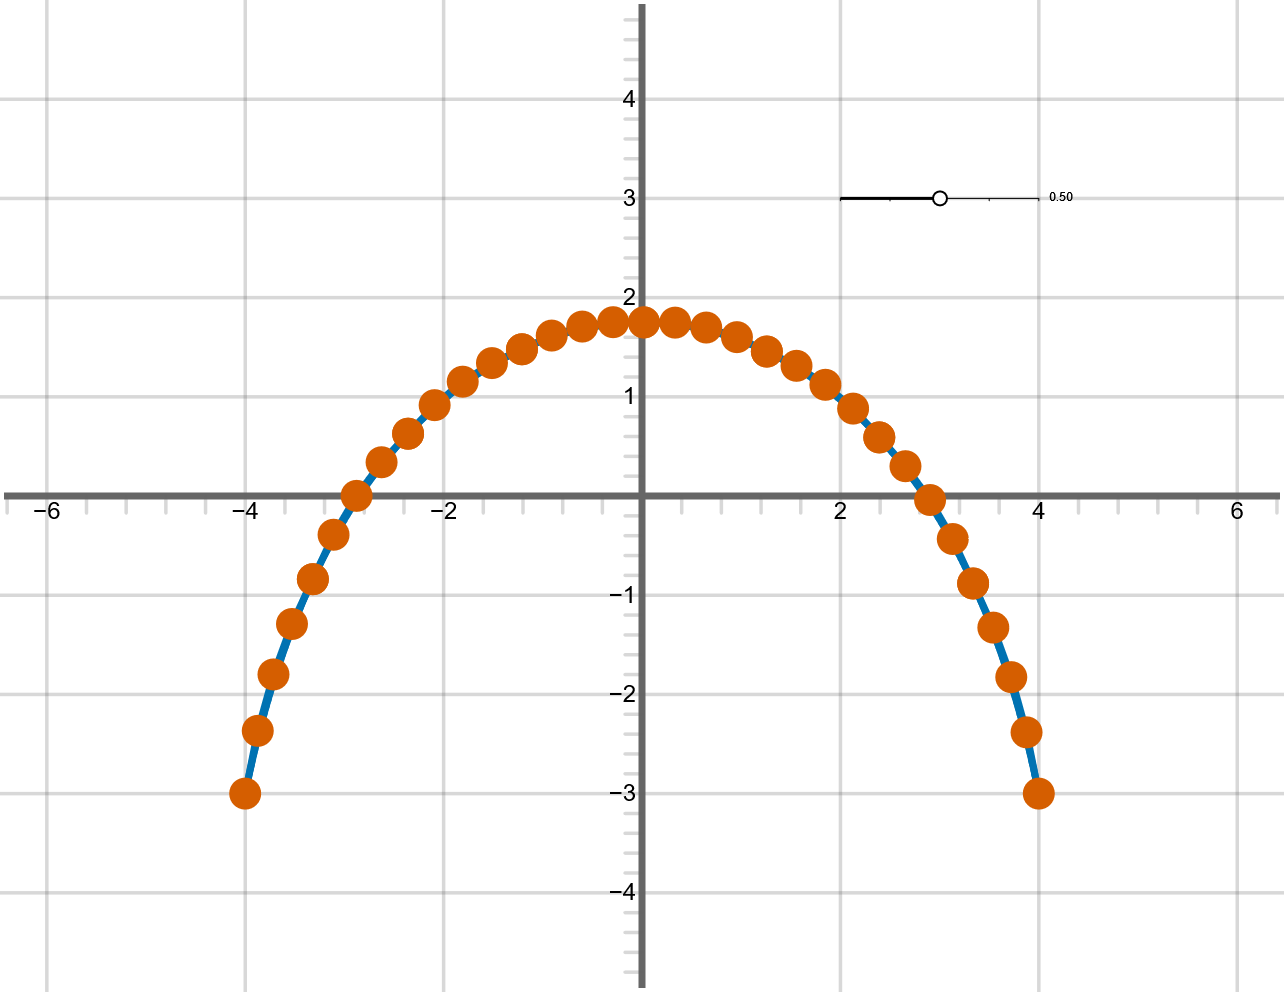
\includegraphics[width = \groupimagewidth]{images/subdivizija-k-3}}
        \caption{Ponavljanje subdivizije.}
        \label{fig:subdivizija-ponavljanje}
    \end{figure}


%    \begin{dokaz}
%        \begin{align*}
%            B_{t_0}(t) = B(t_{0}t) &= \sum_{i=0}^{n}\mathbf{p}_{i}\binom{n}{i}(t_{0}t)^i(1-tt_0)^{n-i}\\
%            &= \sum_{i=0}^{n}\mathbf{p}_{i}\binom{n}{i}(t_{0}t)^i \sum_{j=0}^{n-i} \binom{n-i}{j}(-tt_0)^{j}  \\
%            &= \sum_{i=0}^{n}\mathbf{p}_{i}\binom{n}{i}(tt_0)^i \sum_{j=0}^{n-i} \binom{n-i}{j}(-t)^{j}(t_0)^{j}\\
%            &= \sum_{i=0}^{n}\mathbf{p}_{i}\binom{n}{i}(tt_0)^i \sum_{j=0}^{n-i} \binom{n-i}{j}(-t)^{j}(t_0)^{j}
%        \end{align*}
%        Želimo dobiti
%
%        \begin{align*}
%            \sum_{i=0}^{n}\p_{0}^i(t_0)\binom{n}{i}t^i(1-t)^{n-i} = \sum_{i=0}^{n}\binom{n}{i}t^i(1-t)^{n-i}  \sum_{j=0}^{n-i} \binom{n-i}{j}t_0^j(1-t_0)^{n-i-j}  \p_{j}
%        \end{align*}
%
%    \end{dokaz}

    \subsection{Ekstrapolacija}
    Ker so Bernsteinovi bazni polinomi definirani za vsa realna števila $t$, lahko Bézierjeve krivulje rišemo tudi izven domene $[0,1]$.
    Recimo, da želimo neko Bézierjevo krivuljo risati na domeni $[0,t_0]$, kjer je $t_0>1$.
    Bézierjevo krivuljo na domeni $[0,t_0]$ lahko predstavimo kot Bézierjevo krivuljo na domeni $[0,1]$.
    Pri tem kontrolne točke krivulje preberemo iz de Casteljaujeve sheme, kakor smo to storili za točke krivulje  $B_{t_0-}$ v prejšnjem razdelku. Na sliki~\ref{fig:ekstrapolacija} lahko na prvem grafu vidimo risanje krivulje izven intervala $[0,1]$, na drugem pa ekstrapolirano krivuljo.
    \begin{figure}[h]
        \captionsetup[subfigure]{labelformat=empty}
        \centering
        \subfloat[pred ekstrapolacijo]{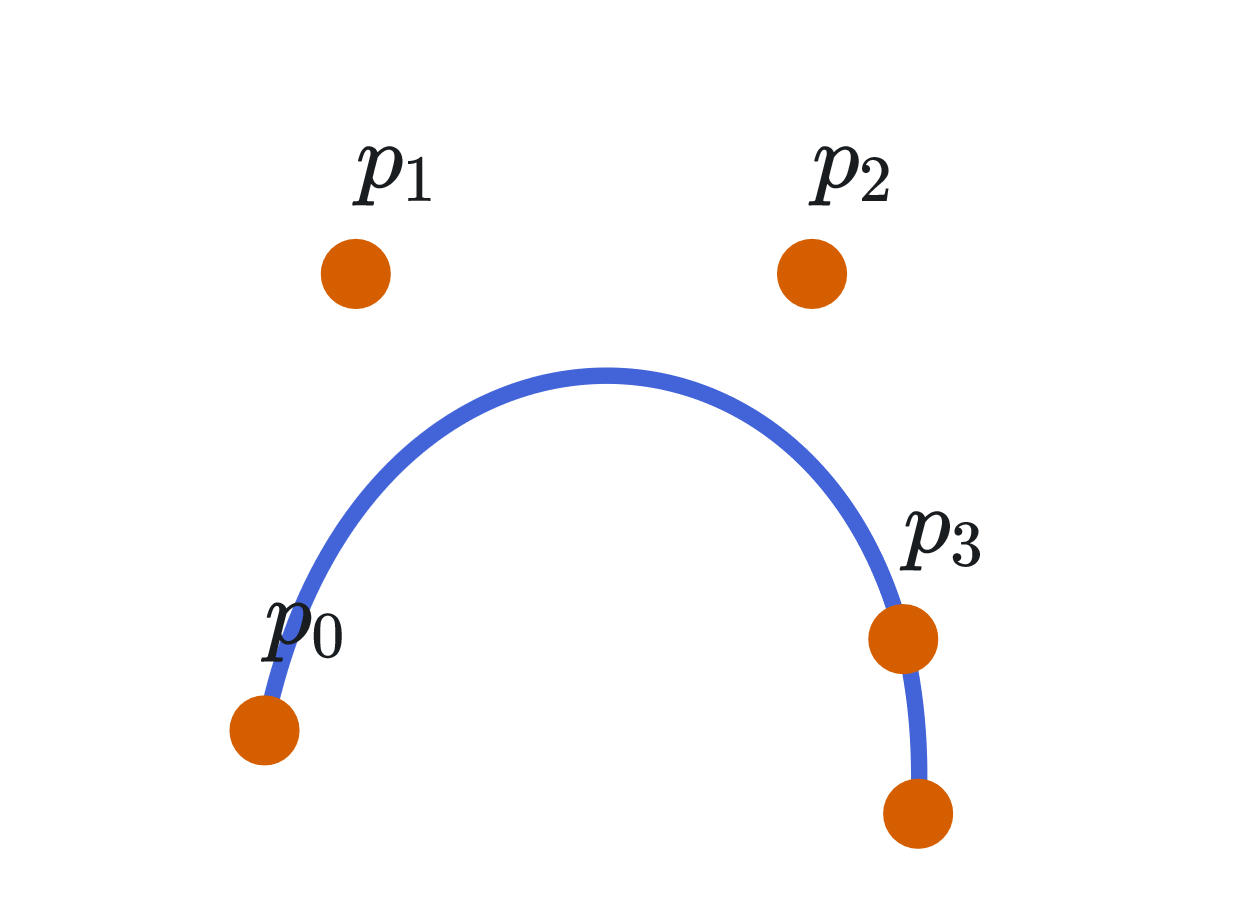
\includegraphics[width = \groupimagewidth]{images/extrapolation-before}}
        \qquad
        \subfloat[po ekstrapolaciji]{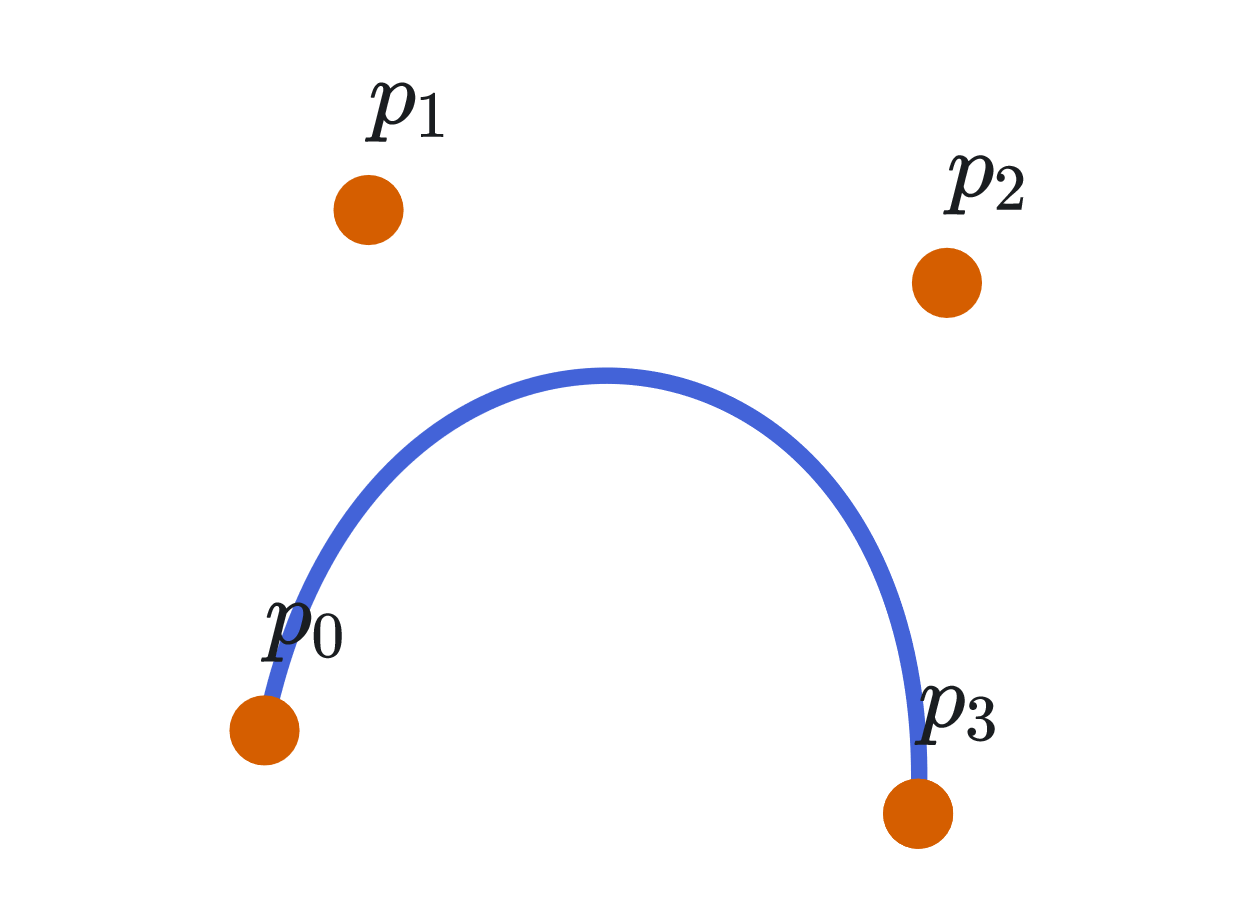
\includegraphics[width = \groupimagewidth]{images/extrapolation-after}}
        \caption{Ekstrapolacija Bézierjeve krivulje.}
        \label{fig:ekstrapolacija}
    \end{figure}

    \subsection{Višanje stopnje}
    Nekateri algoritmi v CAD/CAGD sistemih za vhod potrebujejo dve Bézierjevi krivulji iste stopnje.
    Recimo, da imamo Bézierjevo krivuljo $\B$ stopnje $n$, ki jo želimo predstaviti kot Bézierjevo krivuljo stopnje $n+1$.
    Upoštevajoč $1-t+t=1$, lahko parametrizacijo krivulje $\B$ zapišemo tudi kot
    \begin{align}
        \B(t) = (1-t)\B(t)+t\B(t) = \sum_{i=0}^{n}\mathbf{p}_{i}(1-t)B_i^n(t) +\sum_{i=0}^{n}\mathbf{p}_{i}tB_i^n(t). \label{eq:visanje-param}
    \end{align}
    Če sedaj zvezi za Bernsteinove bazne polinome
    \begin{align*}
    (1-t)
        B_i^n(t) &= & \frac{n+1-i}{n+1} \binom{n+1}{i}&t^i(1-t)^{n+1-i} & &=\frac{n+1-i}{n+1}B_{i}^{n+1}(t), \\
        % &= \frac{n!}{(n-i)!i!}t^i(1-t)^{n+1-i}   &=\frac{n+1-i}{n+1}\frac{(n+1)!}{(n+1-i)!i!}t^i(1-t)^{n+1-i}
        tB_i^n(t) &= & \frac{i+1}{n+1}\frac{(n+1)!}{(n-i)!(i+1)!}&t^{i+1}(1-t)^{n+1-i-1} & &= \frac{i+1}{n+1}B_{n+1}^{n+1}(t),
        %t\binom{n}{i}t^i(1-t)^{n-i} \\
        %&= \frac{n!}{(n-i)!i!}t^{i+1}(1-t)^{n+1-i-1} \\
    \end{align*}
    vstavimo v izraz~\ref{eq:visanje-param}, dobimo
    \begin{align*}
        \B(t) &= \sum_{i=0}^{n}\mathbf{p}_{i}\frac{n+1-i}{n+1}B_{i}^{n+1}(t) +\sum_{i=0}^{n}\mathbf{p}_{i}\frac{i+1}{n+1}B_{i+1}^{n+1}(t)\\
        &= \sum_{i=0}^{n}\mathbf{p}_{i}\frac{n+1-i}{n+1}B_{i}^{n+1}(t) +\sum_{i=1}^{n+1}\mathbf{p}_{i-1}\frac{i}{n+1}B_{i}^{n+1}(t).
%&=\mathbf{p}_{0} + \sum_{i=1}^{n}\left(\mathbf{p}_{i}\frac{n+1-i}{n+1} + \mathbf{p}_{i-1}\frac{i}{n+1}\right)B_{i}^{n+1}(t)+\mathbf{p}_{n}.
    \end{align*}
    Od tod sledi, da lahko krivuljo $\B$ predstavimo kot Bézierjevo krivuljo stopnje $n+1$ s kontrolnimi točkami \[c_0=\p_0, \quad c_i=\mathbf{p}_{i}\frac{n+1-i}{n+1} + \mathbf{p}_{i-1}\frac{i}{n+1},\quad c_{n+1}=\p_n. \]
    Oglejmo si kako višanje stopnje izgleda na neki krivulji.
    Na sliki~\ref{fig:višanje} je na prvem grafu narisana Bézierjeva krivulja stopnje $3$.
    Na drugem grafu, smo stopnjo krivulje zvišali za $1$, na tretjem in četrtem grafu pa smo naredili $10$ oziroma $20$ višanj stopnje začetne krivulje.
    Krivulja je na vseh grafih enaka, imamo le več kontrolnih točk.
    Opaziti je tudi možno, da so kontrolne točke z vsakim višanjem stopnje bližje začetni krivulji, kontrolni poligon pa se zmerom bolj prilega začetni krivulji.
    \begin{figure}[h]
        \captionsetup[subfigure]{labelformat=empty}
        \centering
        \subfloat[začetna krivulja]{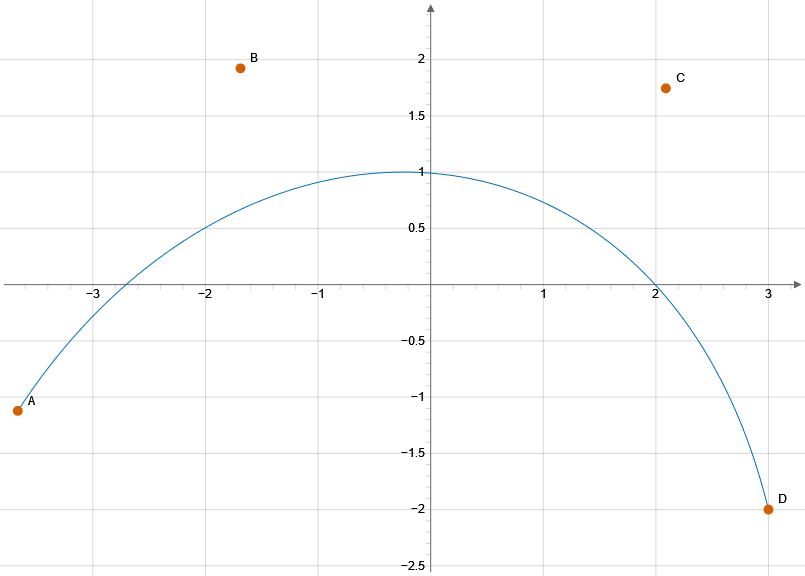
\includegraphics[width = \groupimagewidth]{images/dvig-prej}}
        \qquad
        \subfloat[eno višanje]{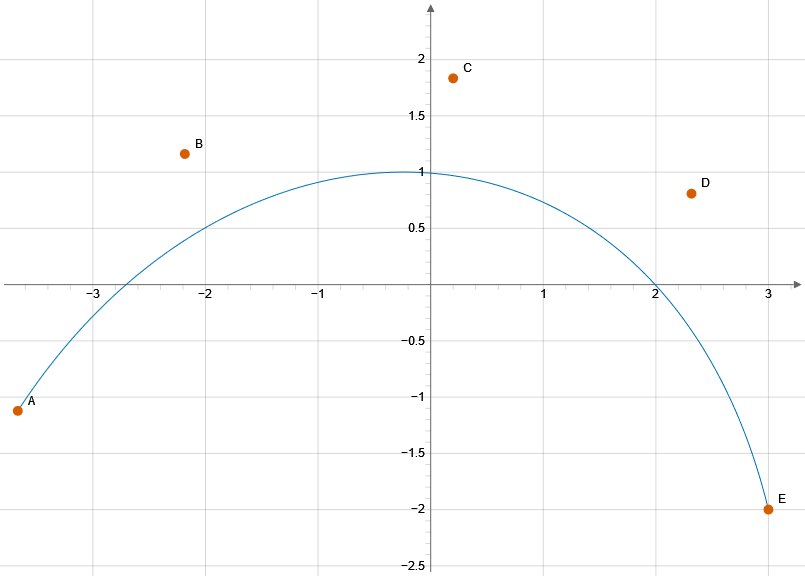
\includegraphics[width = \groupimagewidth]{images/dvig-po}} \\
        \subfloat[10 višanj]{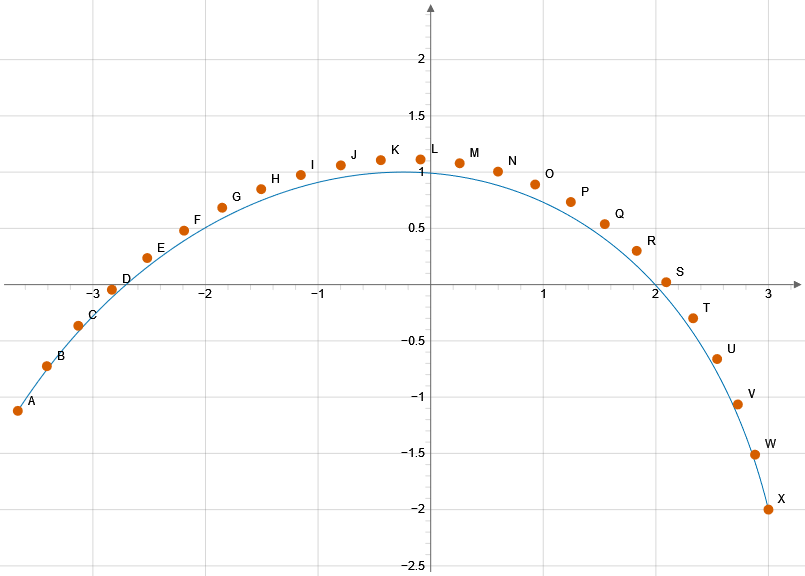
\includegraphics[width = \groupimagewidth]{images/dvig-n}}
        \qquad
        \subfloat[20 višanj]{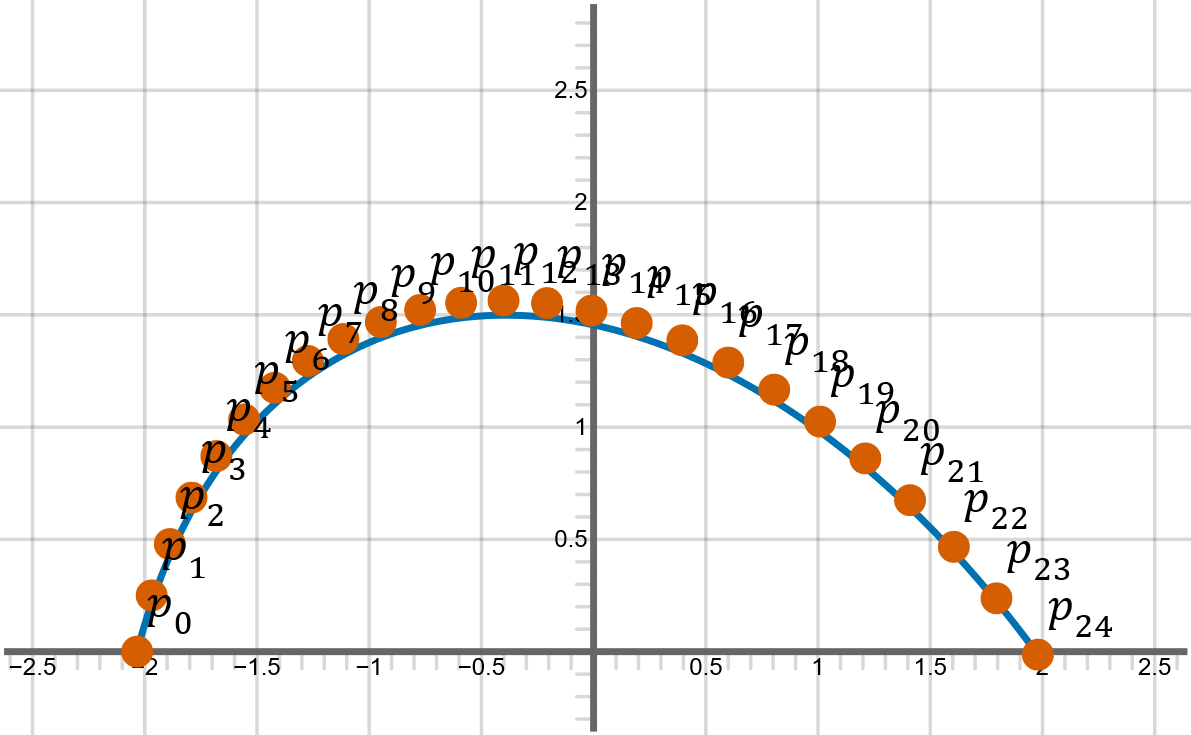
\includegraphics[width = \groupimagewidth]{images/dvig-n2}}
        \caption{Višanje stopnje Bézierjeve krivulje.}
        \label{fig:višanje}
    \end{figure}

    \subsection{Odvodi Bézierjeve krivulje}
    V kasnejših razdelkih bomo potrebovali odvode Bézierjevih krivulj, zato jih na tem mestu izpeljimo.
    Z upoštevanjem izreka o odvodu Bernsteinovih baznih polinomov~\ref{izrek:bernstein-odvod}, dobimo naslednje
    \begin{align*}
        \mathbf{B}'(t) &=   &  &  &\left(\sum_{i=0}^{n}\p_{i}B_i^n(t)\right)' & & & =n \sum_{i=0}^{n}\p_{i}\left(B_{i-1}^{n-1}(t) - B_i^{n-1}(t)\right) \\
        &=            &  & &n \left( \sum_{i=1}^{n}\p_{i}B_{i-1}^{n-1}(t) - \sum_{i=0}^{n-1}\p_{i}B_i^{n-1}(t)\right) & & &= n \sum_{i=0}^{n-1}(\p_{i+1}-\p_{i})B_i^{n-1}(t).
    \end{align*}
    Za krajše zapise višjih odvodov Bézierjeve krivulje, bomo uvedli operator  \textit{prema diferenca}, ki ga označimo z $\Delta$.
    Operator deluje na zaporedni točki $\p_i$, definiramo pa ga rekurzivno kot
    \[\Delta^0\p_i=\p_i,\quad \Delta\p_i=\p_{i+1}-\p_{i}, \quad \Delta^k\p_i=\Delta^{k-1}\p_{i+1}-\Delta^{k-1}\p_{i}.\]
    Za naravno število $k$ lahko v zaključeni obliki podamo ekvivalenten zapis
    \[ \Delta^k\p_i= \sum_{j=0}^k\binom{k}{j}(-1)^{k-j}\p_{i+j}.\]
    \begin{opomba}
        Iz definicije je očitno, da je operator $\Delta^k$ definiran le na kontrolnih točkah z indeksi manjšimi ali enakimi $n-k$.
    \end{opomba}
    \noindent Odvode Bézierjeve krivulje lahko sedaj predstavimo s pomočjo preme diference.
    \begin{izrek}
        \label{izrek:odvod}
        Naj bo $\mathbf{B}$ Bézierjeva krivulja s kontrolnimi točkami $\p_i$, $i=0,1,\ldots,n$.
        Za njene odvode velja
        \[ \mathbf{B}^{(k)}(t) = \frac{n!}{(n-k)!} \sum_{i=0}^{n-k}\Delta^{k}\p_{i}B_i^{n-k}(t),\quad k=0,1,\ldots,n.\]
    \end{izrek}
    \noindent Izrek je enostavno dokazati s pomočjo indukcije, zato bomo dokaz izpustili.
    \newpage

    \section{Racionalne Bézierjeve krivulje}
    Vseh krivulj ne moremo opisati s polinomskimi Bézierjevimi krivuljami.
    Med njimi so tudi takšne, ki so za CAGD sisteme zelo pomembne, na primer izseki krožnice.
    Za opis takšnih krivulj lahko posežemo po racionalnih Bézierjevih krivuljah.
    Racionalno Bézierjevo krivuljo stopnje $n$ v $\R^d$ dobimo tako, da Bézierjevo krivuljo stopnje $n$ v $\R^{d+1}$ projiciramo na hiperravnino $w=1$.
    Točke iz $\R^{d+1}$ pri tem definiramo kot $(w,x_1,\ldots,x_n)$, projekcijo pa s predpisom $(w,\mathbf{x})\to(1,\frac{\mathbf{x}}{w})$.
    Takšna izpeljava privede do naslednje definicije.
    \begin{definicija}
        \label{def:racionalna}
        Racionalna Bézierjeva krivulja stopnje $n\in\N$ je racionalna krivulja podana s kontrolnimi točkami $\p_i\in\R^d$ in \textit{utežmi} $w_i\in\R$, $i=0,1,\ldots,n$, ter parametrizacijo $\mathbf{R}:[0,1]\to \R^d$  določeno s predpisom \[\mathbf{R}(t) = \frac{\sum^{n}_{i=0}w_i\p_i B^n_i(t)}{\sum^{n}_{i=0}w_i B^n_i(t)}.\]
    \end{definicija}
    \noindent Uteži so prosti parametri, ki jih lahko uporabimo pri oblikovanju.
    Kadar so vse uteži enake, je racionalna Bézierjeva krivulja enaka polinomski Bézierjevi krivulji z istimi kontrolnimi točkami.
    Da bi se izognili težavam pri deljenju z $0$ ponavadi privzamemo, da so vse uteži pozitivne.
    Vpliv uteži si poglejmo na sliki~\ref{fig:uteži}.
    Utež spreminjamo le pri kontrolni točki $\p_1$, vse ostale uteži puščamo enake $1$.
    Na grafu (a) je utež nastavljena na število $1$, krivulja na sliki je zato polinomska Bézierjeva krivulja.
    Na grafoma (b) in (c) lahko vidimo, da se z višanjem uteži, krivulja bliža točki $\p_1$.
    Na grafu (c) pa lahko vidimo, da se z nižanjem uteži, krivulja od točke $\p_1$ oddaljuje.
    \begin{figure}[h]
        \centering
        \subfloat[]{\includegraphics[width = \groupimagewidth]{images/racionalnaw1}}
        \qquad
        \subfloat[]{\includegraphics[width = \groupimagewidth]{images/racionalnaw2}}\\
        \subfloat[]{\includegraphics[width = \groupimagewidth]{images/racionalnaw4}}
        \qquad
        \subfloat[]{\includegraphics[width = \groupimagewidth]{images/racionalnaw05}}
        \caption{Vpliv uteži na racionalno Bézierjevo krivuljo.}
        \label{fig:uteži}
    \end{figure}

    Iz zapisa parametrizacije v definiciji~\ref{def:racionalna} lahko hitro vidimo, da množenje vseh uteži s poljubnim neničelnim številom krivulje ne spremeni.
    Tako lahko brez izgube splošnosti poljubno utež fiksiramo na $1$.
    Naslednji izrek pa pove, da lahko to storimo za dve uteži.
    \begin{izrek}
        \label{izrek:racionalne-utezi-1}
        Racionalno Bézierjevo krivuljo s pozitivnimi utežmi $w_i$ in parametrizacijo $\mathbf{R}$, lahko reparametriziramo v parametrizacijo $\mathbf{\tilde{R}}$ s pozitivnimi utežmi $\tilde{w}_i$ tako, da velja $\tilde{w}_0=\tilde{w}_{n}=1.$
    \end{izrek}
    \noindent Dokaz izreka bo konstrukcijske narave.
    Našli bomo torej uteži $\tilde{w}_i$, katere lahko zamenjamo z utežmi $w_i$ tako, da ohranimo isto krivuljo.
    \begin{dokaz}
        Naj bo $\mathbf{R}$ racionalna Bézierjeva funkcija s poljubnimi pozitivnimi utežmi.
        Uporabimo reparametrizacijsko funkcijo $\varphi(t):[0,1]\to[0,1]$ s predpisom $\varphi(t)=\frac{t}{\rho(1-t)+t}$, kjer je $\rho$ pozitivno realno število.
        Če reparametrizacijsko funkcijo vstavimo v $i$-ti Bernsteinov bazni polinom dobimo naslednje
        \begin{align*}
            B^n_i(\varphi(t)) &=  \binom{n}{i}\left(\frac{t}{\rho (1-t)+t}\right)^i\left(1-\frac{t}{\rho (1-t)+t}\right)^{n-i} \\
            &=  \binom{n}{i}\left(\frac{t}{\rho (1-t)+t}\right)^i\left(\frac{\rho(1-t)}{\rho (1-t)+t}\right)^{n-i} \\
            &= \binom{n}{i}\frac{\rho^{n-1}t^{i}(1-t)^{n-i}}{(\rho(1-t)+t)^n} =  \frac{\rho^{n-1}}{(\rho(1-t)+t)^n}B^n_i(t).
        \end{align*}
        Reparametrizirane Bernsteinove bazne polinome sedaj vstavimo v parametrizacijo racionalne Bézierjeve krivulje, da dobimo
        \[\mathbf{\tilde{R}}(t)=\mathbf{R}(\varphi(t)) = \frac{\sum^{n}_{i=0}\rho^{n-i}w_i\p_i B^n_i(t)}{\sum^{n}_{i=0}\rho^{n-i}w_i B^n_i(t)}. \]
        Nove uteži izrazimo s starimi $\hat{w}_i=\rho^{n-i}w_i$.
        Želimo, da bi veljalo $\hat{w}_0=\hat{w}_n$, zato nastavimo $\rho= \sqrt[n]{\frac{w_n}{w_0}}$.
        Ker velja $\hat{w}_n=w_n$ lahko uteži $\hat{w}_i$ delimo z utežjo $w_n$, da dobimo željene uteži \[\tilde{w_i}=\frac{1}{w_n}\hat{w_i} = \frac{w_i}{\sqrt[n]{w^{i}_nw_0^{n-i}}}.\]
    \end{dokaz}
    \begin{posledica}
        Z uvedbo racionalnih Bézierjevih krivulj smo dobili le $n-1$ dodatnih prostih parametrov, glede na polinomske Bézierjeve krivulje z istim številom kontrolnih točk.
    \end{posledica}
    \begin{opomba}
        Če velja $w_0=w_n=1$ pravimo, da je racionalna Bézierjeva krivulja predstavljena v \textit{standardni formi}.
    \end{opomba}
    Brez dokaza povejmo, da lastnosti Bézierjevih krivulj, ki smo jih podali v izreku~\ref{izrek:lastnosti-bezierjevih-krivulj}, veljajo tudi za racionalne Bézierjeve krivulje s pozitivnimi utežmi.
    Subdiviziranje, ekstrapoliranje in višanje stopnje polinomske Bézierjeve krivulje lahko na racionalne Bézierjeve krivulje stopnje $d$ razširimo tako, da krivuljo zapišemo kot polinomsko Bézierjevo krivuljo stopnje $d+1$ s kontrolnimi točkami  $(w_i,w_{i}\p_i)\in R^{d+1}$.
    Polinomsko krivuljo nato subdiviziramo/ekstrapoliramo/ji zvišamo stopnjo in iz dobljenih kontrolnih točk $(\tilde{w}_i,\tilde{w}_{i}\tilde{\p}_i)\in\R^{d+1}$ preberemo nove kontrolne točke $\tilde{\p_i}\in\R^d$ in uteži $\tilde{w_i}\in\R$.
    Pri takšnem procesu samo ekstrapolacija ne ohranja pozitivnosti uteži.
    Primere si lahko ogledamo na sliki~\ref{fig:razsirjene-metode}.
    \begin{figure}[h]
        \centering
        \subfloat[začetna krivulja]{\includegraphics[width = \groupimagewidth]{images/racionalna-start}}
        \qquad
        \subfloat[subdivizija]{\includegraphics[width = \groupimagewidth]{images/racionalna-subdivizija}}\\
        \subfloat[ekstrapolacija]{\includegraphics[width = \groupimagewidth]{images/racionalna-ekstrapolirana}}
        \qquad
        \subfloat[višanje stopnje]{\includegraphics[width = \groupimagewidth]{images/racionalna-dvig}}
        \caption{Subdivizija, ekstrapolacija ter višanje stopnje racionalne Bézierjeve krivulje.}
        \label{fig:razsirjene-metode}
    \end{figure}
%    Interpolacijo točk lahko dokažemo na podoben način, kakor smo to storili pri dokazu izreka~\ref{izrek:lastnosti-bezierjevih-krivulj}.
%    Da dokažemo, da je racionalna Bézierjeva krivulja afino invariantna, ter da leži znotraj konveksne ovojnice kontrolnih točk, pa posežemo po naslednjem zapisu.
%    \[\mathbf{R}(t)=\sum^n_{i=0}\p_i N^n_i, \quad N^n_i(t)\coloneqq \frac{w_i B^n_i(t)}{\sum^n_{i=0}w_i B^n_i(t)}\]
%    Če pri dokazu izreka~\ref{izrek:lastnosti-bezierjevih-krivulj} namesto Bernsteinovih polinomov $B_i^n(t)$ vstavimo funkcijo $N^n_i$ iz zgornjega zapisa, dobimo dokaz lastnosti za racionalne Bézierjeve krivulje.

    \subsection{De Casteljaujev algoritem za racionalne Bézierjeve krivulje}
    Točke racionalnih Bézierjevih krivulj dimenzije $d$ bi lahko računali s pomočjo de Casteljaujevega algoritma za polinomske Bézierjeve krivulje stopnje $d+1$, na podoben način kot smo v prejšnjem razdelku razširili subdivizijo, ekstrapolacijo in višanje stopnje krivulje.
    Takšno računanje točk se izkaže za nestabilno~\ref{placeholder}, zato na tem mestu podamo razširitev de Casteljaujevega algoritma za racionalne Bézierjeve krivulje~\ref{alg:racionalni-decasteljau}, ki točke racionalne Bézierjeve krivulje računa stabilno~\ref{placeholder}.
    \begin{algorithm}[h!]
        \caption{Racionalni de Casteljaujev algoritem}
        \begin{algorithmic}
            \State $\p \gets \p_0,\p_1,\dots,\p_n$
            \State $w\gets w_0,w_1,\dots,w_n$
            \For{$i = 0,1,\dots n$}
                \State $\p_i^0(t)=\p_i$
                \State $w_i^0(t)=w_i$
            \EndFor
            \For{$r = 1,2,\dots n$}
                \For{$i=0,1,\dots,n-r$}
                    \State $w_i^r(t)=(1-t)w_{i}^{r-1}(t)+tw_{i+1}^{r-1}(t)$
                    \State $\p_i^r(t)=(1-t)\frac{w_{i}^{r-1}(t)}{w_{i}^{r}(t)}\p_i^{r-1}(t)+t\frac{w_{i+1}^{r-1}(t)}{w_{i}^{r}(t)}\p_{i+1}^{r-1}(t)$
                \EndFor
            \EndFor
            \State \Return $\p_0^n(t)$
        \end{algorithmic}\label{alg:racionalni-decasteljau}
    \end{algorithm}

    \noindent Brez dokaza z naslednjim izrekom podajmo pravilnost algoritma~\ref{alg:racionalni-decasteljau}.
    \begin{izrek}
        Za vmesne točke $\p_i^r(t)$ iz algoritma~\ref{alg:racionalni-decasteljau} in poljubno realno število $t$ velja izraz
        \[\p_i^r(t)= \frac{\sum^{r}_{j=0}w_{i+j}\p_{i+j} B^r_j(t)}{\sum^{n}_{i=0}w_{i+j} B^r_j(t)}. \]
    \end{izrek}

    \subsection{Farinove točke}
    Uporabniku CAGD sistema želimo nuditi čim bolj naraven način kontroliranja uteži racionalne Bézierjeve krivulje.
    V ta namen lahko uteži predstavimo s \textit{Farinovimi točkami}.
    Farinove točke ležijo na daljicah kontrolnega poligona, kjer $i$-ta Farinova točka $\mathbf{f}_i$ deli $i$-to daljico kontrolnega poligona v razmerju $w_{i+1}:w_{i}$.
    Slednje lahko zapišemo kot \[\frac{|\mathbf{f}_i-\p_i|}{|\mathbf{f}_i-\p_{i+1}|} = \frac{w_{i+1}}{w_{i}}.\]
    S kontrolnimi točkami in utežmi lahko Farinove točke izrazimo takole
    \[\mathbf{f}_i \coloneqq \frac{w_{i}}{w_{i}+w_{i+1}}\p_i +  \frac{w_{i+1}}{w_{i}+w_{i+1}}\p_{i+1}.\]
    Da bi uporabnik lahko s Farinovimi točkami kontroliral uteži, pa želimo obratno — s Farinovimi točkami želimo izraziti uteži.
    Brez izgube splošnosti lahko za prvo utež izberemo $w_0=1$.
    Ostale točke lahko nato rekurzivno izračunamo s pomočjo naslednjega izraza
    \[w_{i+1} = w_i\frac{|\mathbf{f}_i-\p_i|}{|\mathbf{f}_i-\p_{i+1}|}.\]
    Po želji lahko uteži tudi standardiziramo s pomočjo formule \[\tilde{w}_{i} = \frac{w_i}{\sqrt[n]{w_n^i}},\]
    ki sledi iz dokaza izreka~\ref{izrek:racionalne-utezi-1}.

    Na sliki~\ref{fig:farinove-tocke} si lahko ogledamo delovanje Farinovih točk.
    Uteži na sliki niso standardizirane zato, da lahko bolje vidimo razmerja med njimi.
    Na grafu (a) Farinove točke ležijo na sredini pripadajočih daljic.
    Posledično so vsa razmerja $|\p_i-\mathbf{f}_i|:|\p_{i+1}-\mathbf{f}_i|$ enaka in vse uteži enake $1$.
    Na grafu (b) lahko vidimo, da se s premikom prve Farinove točke bližje k točki $\p_0$, k njej približa tudi krivulja.
    Utež $w_1$, ki predstavlja razmerje $|\p_0-\mathbf{f}_0|:|\p_{1}-\mathbf{f}_0|$, je zato manjša kot $1$.
    Na grafu (c) lahko vidimo premik Farinove točke bližje k točki $\p_1$.
    Krivulja se točki približa, utež $w_1$ pa se poveča na več kot $1$.
    Ker na grafoma (b) in (c) druga in tretja Farinova točka ležita na sredini svojih daljic, so uteži $w_1$,$w_2$ in $w_3$ enake.
    Na grafoma (d) in (e) lahko vidimo, kako se krivulja in uteži obnašajo ob premiku druge Farinove točke.
    Na grafoma (f) ter (g) pa lahko vidimo obnašanje krivulje, ko premaknemo prvo ter tretjo Farinovo točko hkrati gor oziroma dol.
    Poglejmo še, kaj se zgodi, če vse tri točke premaknemo pomaknemo tako, da so razmerja na vseh daljicah enaka.
    Na levem grafu slike~\ref{fig:farinove-tocke-2} lahko vidimo, da krivulja izgleda kakor začetna.
    Če uteži standardiziramo, kar smo storili na desnem grafu, vidimo, da je temu res tako.
    Da bi preprečili takšno izbiro Farinovih točk, lahko po vsakem premiku Farinove točke uteži standardiziramo, ter ponovno izračunamo Farinove točke.
    \begin{figure}[h!]
        \centering
        \subfloat[]{\includegraphics[width = \groupimagewidth]{images/farinove-tocke-premik-0}}\\
        \subfloat[]{\includegraphics[width = \groupimagewidth]{images/farinove-tocke-premik-leva-1}}
        \qquad
        \subfloat[]{\includegraphics[width = \groupimagewidth]{images/farinove-tocke-premik-leva-2}}
        \qquad
        \subfloat[]{\includegraphics[width = \groupimagewidth]{images/farinove-tocke-premik-zgornja-1}}
        \qquad
        \subfloat[]{\includegraphics[width = \groupimagewidth]{images/farinove-tocke-premik-zgornja-2}}
        \qquad
        \subfloat[]{\includegraphics[width = \groupimagewidth]{images/farinove-tocke-premik-obe-1}}
        \qquad
        \subfloat[]{\includegraphics[width = \groupimagewidth]{images/farinove-tocke-premik-obe-2}}
        \caption{Kontroliranje krivulje s Farinovimi točkami.}
        \label{fig:farinove-tocke}
    \end{figure}

    \begin{figure}[h!]
        \centering
        \subfloat[]{\includegraphics[width = \groupimagewidth]{images/farinove-tocke-premik-vsetri-0}}
        \qquad
        \subfloat[]{\includegraphics[width = \groupimagewidth]{images/farinove-tocke-premik-vsetri-1}}
        \caption{Krivulja z enakimi premiki vseh Farinovih točk, pred in po standardizaciji.}
        \label{fig:farinove-tocke-2}
    \end{figure}
    \newpage

%    \subsubsection{Izsek krožnice}
%    V uvodu podrazdelka smo povedali, da se nekaterih krivulj ne da opisati z navadnimi Bézierjevimi krivuljami.
%    Kot enega izmed primerov smo podali izsek krožnice.
%    V tem delu podrazdelka bomo izpeljali kontrolne točke in uteži racionalne Bézierjeve krivulje, da bo krivulja predstavljala izsek krožnice s polmerom $R$ in \mycomment{kotom $\alpha$}.
%    Izsek krožnice bomo podali s kvadratičnimi racionalnimi Bézierjevimi krivuljami.
%    Za konstrukcijo imamo na voljo kontrolne točke $\p_0,\p_1$ in $\p_2$, ter uteži $w_0,w_1$ in $w_2$.
%    Iz izreka~\ref{izrek:racionalne-utezi-1} sledi, da lahko robni uteži fiksiramo na $w_0=w_2=1$.
%    Točki $\p_0$ in $\p_2$ morata ležati na začetku ter koncu izseka krožnice, saj racionalne Bézierjeve krivulje interpolirajo končne točke.
%    Ker so racionalne Bézierjeve krivulje afino invariantne, lahko brez izgube splošnosti postavimo točki $\p_0$ in $\p_2$ tako, da velja $\p_0=-\p_2$.
%    Parametrizacija željene krivulje izgleda takole
%    \[\mathbf{R}(t) = \frac{\sum^{2}_{i=0}w_i\p_i B^2_i(t)}{\sum^{2}_{i=0}w_i B^2_i(t)} = \frac{\p_0 (1-t)^2 + w_1\p_1 2t(1-t) + \p_2 t^2}{(1-t)^2 + w_1 2t(1-t) + t^2}.\]
%    Velja torej $T=R(\frac{1}{2})= \frac{w_1\p_1}{w_1+1}$.
%    Poglejmo si sliko\mycomment{referenca}.
%    Iz nje lahko razberemo zvezi
%    \begin{align*}
%        |OT|=|ST|-|SO| = R - R\sin\frac{\alpha}{2} = R(1-\sin\frac{\alpha}{2})\\
%        |O\p_1| = |S\p_1|-|SO| = \frac{R}{\sin\frac{\alpha}{2}} - R\sin\frac{\alpha}{2} = R\frac{1-\sin^2\frac{\alpha}{2}}{\sin\frac{\alpha}{2}}
%    \end{align*}
%    Iz zveze $\frac{|OT|}{|O\p_1|} = \frac{\sin\frac{\alpha}{2}}{\sin\frac{\alpha}{2}+1} = \frac{w_1}{w_1+1}$ nato sledi $w_1=\sin\frac{\alpha}{2}$.
%    Pričakujemo, da bo točka $\p_1$ oblike $(0,y)$.
%    Velja torej $|O\p_1|=y=R\frac{1-\sin^2\frac{\alpha}{2}}{\sin\frac{\alpha}{2}}$.
%
%%
%%
%%%    po komponentah pa
%%%    \begin{align*}
%%%        x(t) &= \frac{(1-t)^2 + w_1R\cos\left(\frac{\alpha}{2}\right) 2t(1-t) + \cos(\alpha)t^2}{(1-t)^2 + w_1 2t(1-t) + t^2} \\
%%%        y(t) &= \frac{w_12t(1-t)R\sin\left(\frac{\alpha}{2}\right) + \sin(\alpha)t^2}{(1-t)^2 + w_1 2t(1-t) + t^2}.
%%%    \end{align*}
%%    Tangenta na enotsko krožnico je v točki $(1,0)$ vzporedna z ordinatno osjo, zato mora veljati $x'(0)=0$.
%%    \mycomment{Odvod racionalne Bézierjeve krivulje v točki $(1,0)$ je enak $2(\p_{1}-\p_{0}) = 2\left(R\sin\left(\frac{\alpha}{2}\right)-r,R\cos\left(\frac{\alpha}{2}\right)\right)$.}
%%    Iz česar sledi $R=\frac{r}{\cos\left(\frac{\alpha}{2}\right)}$.
%%    \begin{align*}
%%        w_1\left(\frac{r}{\sin\left(\frac{\alpha}{2}\right)}-r\right)\sin\left(\frac{\alpha}{2}\right)  &= r\sin\left(\frac{\alpha}{2}\right) - \frac{r}{2}\sin(\alpha) \\
%%        w_1 &= \frac{r\sin\left(\frac{\alpha}{2}\right) - \frac{r}{2}\sin(\alpha)}{\left(\frac{r}{\sin\left(\frac{\alpha}{2}\right)}-r\right)\sin\left(\frac{\alpha}{2}\right) }
%%    \end{align*}
%%
%%
%%    Zaradi simetrije mora krivulja v $t=\frac{1}{2}$ interpolirati točko $\left(\cos\left(\frac{\alpha}{2}\right),\sin\left(\frac{\alpha}{2}\right)\right)$ iz česar sledi
%%    \begin{align*}
%%        x\left(\frac{1}{2}\right) &= \frac{\frac{1}{4} +  \frac{1}{2}w_1R\cos\left(\frac{\alpha}{2}\right) + \frac{1}{4}\cos(\alpha)}{\frac{1}{4}+ w_1\frac{1}{2} + \frac{1}{4}} = \frac{ \frac{1}{2} + w_1R\cos\left(\frac{\alpha}{2}\right) + \frac{1}{2}\cos(\alpha)}{1+w_1} = \cos\left(\frac{\alpha}{2}\right) \\
%%        y\left(\frac{1}{2}\right) &= \frac{\frac{w_1}{2}R\sin\left(\frac{\alpha}{2}\right) + \frac{1}{4}\sin(\alpha)}{\frac{1}{4}+ w_1\frac{1}{2} + \frac{1}{4}} =  \frac{w_1R\sin\left(\frac{\alpha}{2}\right) + \frac{1}{2}\sin(\alpha)}{1+w_1} = \sin\left(\frac{\alpha}{2}\right).
%%    \end{align*}
%%    Iz enačbe izpostavimo $w_1$
%%    \begin{align*}
%%        \frac{1}{2} + w_1R\cos\left(\frac{\alpha}{2}\right) + \frac{1}{2}\cos(\alpha) &= (1+w_1)\cos\left(\frac{\alpha}{2}\right) \\
%%        w_1R\cos\left(\frac{\alpha}{2}\right) - w_1\cos\left(\frac{\alpha}{2}\right) &= \cos\left(\frac{\alpha}{2}\right)-\frac{1}{2} - \frac{1}{2}\cos(\alpha) \\
%%        w_1(R-1)\cos\left(\frac{\alpha}{2}\right) &= \left(\cos\left(\frac{\alpha}{2}\right)-\frac{1}{2} - \frac{1}{2}\cos(\alpha)\right)
%%    \end{align*}
%%    NEXT
%%    \begin{align*}
%%        w_1R\sin\left(\frac{\alpha}{2}\right) + \frac{1}{2}\sin(\alpha) &= (1+w_1)\sin\left(\frac{\alpha}{2}\right) \\
%%        w_1(R-1)\sin\left(\frac{\alpha}{2}\right)  &= \sin\left(\frac{\alpha}{2}\right) - \frac{1}{2}\sin(\alpha)
%%    \end{align*}
%%
%%    \begin{align*}
%%        \frac{r}{2} + w_1R\cos\left(\frac{\alpha}{2}\right) + \frac{r}{2}\cos(\alpha) &=(1+w_1) r\cos\left(\frac{\alpha}{2}\right) \\
%%        w_1R\cos\left(\frac{\alpha}{2}\right) - w_1r\cos\left(\frac{\alpha}{2}\right) &= r\cos\left(\frac{\alpha}{2}\right)-\frac{r}{2}\cos(\alpha)-\frac{r}{2} \\
%%        w_1(R-r)\cos\left(\frac{\alpha}{2}\right) &= r\cos\left(\frac{\alpha}{2}\right)-\frac{r}{2}\cos(\alpha)-\frac{r}{2} \\
%%        w_1 &=\frac{r\cos\left(\frac{\alpha}{2}\right)-\frac{r}{2}\cos(\alpha)-\frac{r}{2}}{(R-r)\cos\left(\frac{\alpha}{2}\right)}\\
%%        w_1 &=\frac{r\cos\left(\frac{\alpha}{2}\right)-\frac{r}{2}\cos(\alpha)-\frac{r}{2}}{(R=\frac{r}{\cos\left(\frac{\alpha}{2}\right)}-r)\cos\left(\frac{\alpha}{2}\right)}
%%    \end{align*}
%%
%%
%%
%%    \begin{align*}
%%        w_1\left(\frac{r}{\sin\left(\frac{\alpha}{2}\right)}-r\right)\sin\left(\frac{\alpha}{2}\right)  &= r\sin\left(\frac{\alpha}{2}\right) - \frac{r}{2}\sin(\alpha) \\
%%        w_1 &= \frac{r\sin\left(\frac{\alpha}{2}\right) - \frac{r}{2}\sin(\alpha)}{\left(\frac{r}{\sin\left(\frac{\alpha}{2}\right)}-r\right)\sin\left(\frac{\alpha}{2}\right) }
%%    \end{align*}
%%    Izračunajmo sedaj za $r=1$ in $\alpha = \frac{\pi}{2}$. $R=\frac{1}{\cos\left(\frac{\pi}{4}\right)} = \sqrt{2}.$
%%    \[ w_1 = \frac{\frac{\sqrt{2}-1}{2}}{(\sqrt{2}-1)\frac{\sqrt{2}}{2}} = \frac{\sqrt{2}-1}{(\sqrt{2}-1)\sqrt{2}} = \frac{\sqrt{2}}{2} \]
%
    \newpage

    \section{Zlepki Bézierjevih krivulj}
    Če si ponovno ogledamo de Casteljaujev algoritem~\ref{alg:decasteljau}, lahko hitro opazimo, da je časovna kompleksnost algoritma $O(n^2)$.
    Računanje točk kompleksnejše Bézierjeve krivulje, z veliko kontrolnimi točkami,  je zato zamudno.
    Da bi ohranili uporabniku naravno kontrolo krivulj ter hiter izračun točk, posežemo po zlepkih Bézierjevih krivulj.
    \begin{definicija}
        Zlepek krivulj $\mathbf{S}:[a,b]\to \R^d$ nad zaporedjem stičnih točk \[a=u_0 < u\_1 < \cdots < u_{m-1} < u_m = b\] je parametrično podana krivulja stopnje $n\in\N$, katere komponente so odsekoma polinomske funkcije $\mathbf{S}|_{[u_{l-1},u_l]} \in \Pn^d$.
    \end{definicija}
    \noindent Želimo si, da bi zlepki tvorili gladko neprekinjeno krivuljo, saj so takšne krivulje v CAGD sistemih najbolj uporabne.
    Krivulja je po definiciji na posameznih odsekih polinomska in zato tudi gladka, problem je le v stičnih točkah.
    Naj bo
    \[\mathbf{S}(u) = \begin{dcases}
                          \mathbf{S_1}(u) = \sum_{i=0}^n \p_i^{(1)}B_i^n\left(\frac{u-u_0}{\Delta u_0}\right), & u \in [u_0,u_1),  \\
                          \mathbf{S_2}(u) = \sum_{i=0}^n \p_i^{(2)}B_i^n\left(\frac{u-u_1}{\Delta u_1}\right), & u \in [u_1,u_2],
    \end{dcases}\]
    zlepek dveh Bézierjevih krivulj.
    Da bo zlepek zvezen, mora v stični točki $u_1$ veljati $\mathbf{S}_1(u_1) = \mathbf{S}_2(u_1)$ oziroma
    \begin{align}
        \label{c0-zlepek-ref}
        \p_n^{(1)} = \p_0^{(2)}.
    \end{align}
    Takšen zlepek, si lahko ogledamo na sliki~\ref{fig:zlepek-c0}.
    \begin{figure}[h]
        \centering
        \includegraphics[width = 0.50\textwidth]{images/zlepek-c0}
        \caption{$C^0$ zlepek dveh Bézierjevih krivulj.}
        \label{fig:zlepek-c0}
    \end{figure}

    \noindent Da bo zlepek vsaj zvezno odvedljiv, mora veljati~\eqref{c0-zlepek-ref}, morata pa v stični točki sovpadati tudi odvoda $\mathbf{S_1}'(u_1) = \mathbf{S_2}'(u_1)$.
    Iz izreka~\ref{izrek:odvod} sledi, da mora zato veljati
    \begin{align}
        \frac{\p_{n}^{(1)} - \p_{n-1}^{(1)}}{\Delta u_0} = \frac{\p_{1}^{(2)} - \p_{0}^{(2)}}{\Delta u_1}.
    \end{align}
    Upoštevajoč~\eqref{c0-zlepek-ref} lahko enačbo zapišemo tudi kot
    $$\p_{n}^{(1)} =  \p_{0}^{(2)}  = \frac{\Delta u_0\p_{1}^{(2)}}{\Delta u_0+\Delta u_1} + \frac{\Delta u_1\p_{n-1}^{(1)}}{\Delta u_0+\Delta u_1} ,$$
    od koder je moč prebrati geometrijski pomen pogoja.
    Skupna točka $\p_{n}^{(1)} =  \p_{0}^{(2)}$ mora namreč deliti daljico $\p_{n-1}^{(1)}\p_{1}^{(2)}$ v razmerju $\frac{\Delta u_0}{\Delta u_1}$.
    Primer takšnega zlepka si lahko ogledamo na sliki~\ref{fig:zlepek-c1}.
    \begin{figure}[h]
        \centering
        \includegraphics[width = 0.50\textwidth]{images/zlepek-c1}
        \caption{$C^1$ zlepek dveh Bézierjevih krivulj, kjer je $\Delta u_0=\Delta u_1$.}
        \label{fig:zlepek-c1}
    \end{figure}
    Podobno lahko iz izreka~\ref{izrek:odvod} preberemo pogoje gladkosti za $C^r([a,b])$,
    $$ \frac{1}{(\Delta u_0)^k}\Delta^k\p^{(1)}_{n-k}= \frac{1}{(\Delta u_1)^k}\Delta^k\p^{(2)}_{0}, \quad k=0,\dots,r.$$
    Primer $C^2$ oziroma $C^3$ zlepka si lahko ogledamo na sliki~\ref{fig:zlepek-c2} oziroma sliki~\ref{fig:zlepek-c3}.
    \begin{figure}[h]
        \centering
        \includegraphics[width = 0.50\textwidth]{images/zlepek-c2}
        \caption{$C^2$ zlepek dveh Bézierjevih krivulj, kjer je $\Delta u_0=\Delta u_1$.}
        \label{fig:zlepek-c2}
    \end{figure}
    \begin{figure}[h]
        \centering
        \includegraphics[width = 0.50\textwidth]{images/zlepek-c3}
        \caption{$C^3$ zlepek dveh Bézierjevih krivulj, kjer je $\Delta u_0=\Delta u_1$.}
        \label{fig:zlepek-c3}
    \end{figure}
    \newpage




    \subsection{Geometrijska zveznost}
    Da bi zlepki bili gladki ne potrebujemo zvezne odvedljivosti v analitičnem smislu, dovolj je zvezna odvedljivost v geometrijskem smislu.
    \begin{definicija}
        \label{def:geometrijska-zveznost}
        Zlepek krivulj \[\mathbf{s}(u) = \begin{cases}
                                             \mathbf{s_1}(u), & u \in [u_0,u_1),  \\
                                             \mathbf{s_2}(u), & u \in [u_1,u_2],
        \end{cases}\] je $k$-krat geometrijsko zvezno odvedljiv, $G^k$, če v okolici stične točke $u_1$ obstaja takšna regularna reparametrizacijska funkcija $\varphi$, da je $\varphi(u_1)=u_1$ in zlepek krivulj
        \[\mathbf{s}(u) = \begin{cases}
                              \mathbf{s_1}(u), & u \in [u_0,u_1),  \\
                              \mathbf{s_2}(\varphi(u)), & u \in [u_1,u_2],
        \end{cases}\]
        $k$-krat zvezno odvedljiv.
    \end{definicija}
    \noindent Izpeljimo sedaj pogoje gladkosti za $G^k$, $k=0,1,2$.
    Za $G^0$ mora veljati $$\mathbf{s_1}(u_1) =  \mathbf{s_2}(\varphi(u_1))$$ kar je enak pogoj, kakor za $C^0$.
    Za $G^1$ mora veljati prejšnje in $$ \mathbf{s_1'}(u_1) = \mathbf{s_2'}(\varphi(u_1))\varphi'(u_1) = \mathbf{s_2'}(u_1)\varphi'(u_1).$$
    Za $G^2$ pa mora veljati prejšnje ter $$\mathbf{s_1''}(u_1) = \mathbf{s_2''}(\varphi(u_1))(\varphi'(u_1))^2 +  \mathbf{s_2'}(\varphi(u_1))\varphi''(u_1) =\mathbf{s_2''}(u_1)(\varphi'(u_1))^2 +  \mathbf{s_2'}(u_1))\varphi''(u_1).$$
    Če sedaj označimo odvode reparametrizacijske funkcije v točki $u_1$ z $\beta_i = \varphi^{(i)}(u_1)$, lahko pogoje za $G^2$ zveznost izrazimo s povezovalno matriko
    $$
    \begin{bmatrix}
        \mathbf{s_1'}(u_1) \\
        \mathbf{s_1''}(u_1)
    \end{bmatrix}
    =
    \begin{bmatrix}
        \beta_1 & 0         \\
        \beta_2 & \beta_1^2
    \end{bmatrix}  \begin{bmatrix}
                       \mathbf{s_2'}(u_1) \\
                       \mathbf{s_2''}(u_1)
    \end{bmatrix}.$$
    Lahko pa naredimo tudi obratno - pri izbranih $\beta_i$ lahko konstruiramo reparametrizacijsko funkcijo, ki ustreza pogojem $\varphi'>0$,  $\varphi'(u_1)=\beta_1$ in $\varphi'(u_1)=\beta_2$. Vzamemo lahko namreč kar Taylorjev polinom
    $$\varphi(u) = u_1 + \beta_1(u-u_1) + \frac{1}{2}\beta_2(u-u_1)^2.$$

    Oglejmo si sedaj, kako pogoji za geometrijsko zveznost vplivajo na zlepke Bézierjevih krivulj.
    Naj bosta $s_1$ in $s_2$ Bézierjevi krivulji. \mycomment{iz prejšnjega zlepka?}
    Za $G^1$ mora veljati  $\mathbf{s_1'}(u_1) = \beta_1\mathbf{s_2'}(u_1)$, iz česar sledi
    $$\frac{\p_{n}^{(1)} - \p_{n-1}^{(1)}}{\Delta u_0} = \beta_1\frac{\p_{1}^{(2)} - \p_{0}^{(2)}}{\Delta u_1}.$$
    Če označimo sedaj $\alpha_1=  \frac{\beta_1\Delta u_0}{\Delta u_1}$ pa lahko pogoj zapišemo kot
    $$\p_{n}^{(1)} - \p_{n-1}^{(1)}= \alpha_1(\p_{1}^{(2)} - \p_{0}^{(2)}).$$
    Glede na $C^1$ smo torej pridobili prosti parameter, ki ga lahko v CAGD sistemih uporabimo za dodatno kontrolo nad krivuljo.
    $G^1$ zlepek in vpliv izbora $\beta_1$ si lahko ogledamo na sliki~\ref{fig:zlepek-g1}.
    \begin{figure}[h]
        \centering
        \subfloat[$\beta_1=1$]{\includegraphics[width = \groupimagewidth]{images/zlepek-g1}}
        \qquad
        \subfloat[$\beta_1<1$]{\includegraphics[width = \groupimagewidth]{images/zlepek-g1-2}}
        \qquad
        \subfloat[$\beta_1>1$]{\includegraphics[width = \groupimagewidth]{images/zlepek-g1-3}}
        \caption{Vpliv izbora $\beta_1$ pri $G^1$ zlepku.}
        \label{fig:zlepek-g1}
    \end{figure}
%
%    \subsection{Alfa parametrizacije}
%    Pri zlepkih se nam lahko zgodi, da imamo nekatere odseke krajše kakor druge.
%    Pri izbiri ekvidistantnih $t$ dobimo potem razmike na zlepku $s(t_i)-s(t_{i+1})$, ki lahko zelo varirajo.
%    Želeli bi, da so razmiki čimbolj podobni.
%    Pomagamo si lahko tako, da intervale definiramo glede na razdaljo med stičnimi točkami.
%    \[d_i=|T_i-T_{i-1}|^{\alpha}\]
%    \mycomment{NE
%    NE
%    NE
%    Tisto je bilo nekaj drugega. Te alfa parametrizacije so za zlepke!! Ma mentor je najbrz mislil, da bi ne o tem a?
%    Ker to bi prislo prav, ce naredim tudi zlepke PH krivulj (kar naceloma ne bi smelo bit tako problematicno...).
%    }

    \newpage


    \section{PH Krivulje}
    Motivacija: fajn so nam takšne parametrizacije, da se isto hitro premikamo po njih. (ce karkoli rises recimo)
    V poglavju se bomo osredotočili (mogoce celo samo govorili?) o krivuljah v $\R^2$.

    \subsection{Dolžina krivulje kot racionalna funkcija}
    Dolžina krivulje podane s parametrizacijo  $\mathbf{r}(t) = \left(x(t),y(t)\right)$ je definirana z enačbo $\int_0^t \sqrt {x^{'2}(t)+y^{'2}(t)}$.
    Integrandu v enačbi pravimo \textit{parametrična hitrost} krivulje, označimo ga z $\sigma(t)$.
    Idealno bi bilo, da je hitrost $\sigma(t) = 1$ za vsak $t\in [0,t_0]$, saj bi v tem primeru veljalo $s(t)=t$.
    Takšna parametrizacija je zlahka dosegljiva za črte, tudi za odseke krožnice (z rabo trigonometričnih funkcij), v splošnem pa ne.
    Dokaz da nobena krivulja ne more biti parametrizirana z racionalnimi funkcijami svoje dolzine.???

    \subsection{Polinomska parametrična hitrost}
    Kot smo zgoraj dokazali, ne moremo doseči racionalne parametrizacije krivulje, ki bi imela hitrost enako $1$.
    Če krivulje nekoliko omejimo, lahko dosežemo, da bo funkcija hitrosti vsaj polinom.
    To dosežemo tako, da zahtevamo, da je polinom $x^{'2}(t)+y^{'2}(t)$ popoln kvadrat.
    V takšnem primeru se namreč koren v integrandu izraza REFNAENACBO pokrajša, pod integralom pa ostane polinom.
    Krivuljam za katere to drži pravimo \textit{krivulje s pitagorejskimi hodografi} oziroma \textit{PH krivulje}.
    Integral polinoma je tudi polinom, iz česar sledi, da lahko dolžino PH krivulje izračunamo tako, da evalviramo polinom.
    V naslednjih razdelkih bomo videli, da nam tale lastnost omogoča več, kot samo

    \begin{definicija}
        Hodograf krivulje podane s parametrizacijo $\mathbf{r}(t)\in \R^n$ je krivulja katere parametrizacija je odvod parametrizacije prvotne krivulje.
        \mycomment{V primeru, da komponente parametrizacije hodografa krivulje tvorijo
        Krivulja podana s parametrizacijo $\mathbf{r}(t)\in \R^n$ je krivulja s pitagorejskim hodografom, če komponente hodografa tvorijo pitagorejsko $(n+1)$-terko. (???????????????? se tako rece?)}
    \end{definicija}

    Pri konstrukciji Bézierjevih PH krivulj bomo potrebovali polinome, ki tvorijo pitagorejske trojice.
    Pomagali si bomo z naslednjim izrekom.

    \begin{izrek}              % (tvorijo pitagorejsko trojico??)
        Polinomi $a,b$ in $c$ tvorijo pitagorejsko trojico, tj.\ zadoščajo enačbi
        \vspace{-0.3cm}
        \begin{align}
            a^2(t)+b^2(t)=c^2(t), \label{eq:abc}
        \end{align}
        natanko tedaj, ko obstajata tuja si polinoma $u$ in $v$ ter nek polinom  $w$ za katere velja
        \vspace{-0.3cm}
        \begin{align}
            &a(t)=[u^2(t)-v^2(t)]w(t), \nonumber \\
            &b(t)=2u(t)v(t)w(t),        \nonumber \\
            &c(t)=[u^2(t)+v^2(t)]w(t). \label{eq:uvw}
        \end{align}
    \end{izrek}
    \noindent Izrek tudi dokažimo.
    \begin{dokaz}
        \mbox{}\\
        ($\Leftarrow$) Dokaz je enostaven, saj lahko vrednosti polinomov $a$,$b$ in $c$ iz enačbe ~\eqref{eq:uvw} vstavimo v enačbo ~\eqref{eq:abc} in preverimo. \\
        ($\Rightarrow$) Najprej definiramo polinom $w(t)=\gcd(a(t),b(t),c(t))$.
        Pri tako definiranem polinomu $w$, so si polinomi $\tilde{a}(t)=\frac{a(t)}{w(t)}, \tilde{b}(t)=\frac{b(t)}{w(t)}, \tilde{c}(t)=\frac{c(t)}{w(t)}$ tuji in zadoščajo enačbi $\tilde{a}^2(t)+\tilde{b}^2(t)=\tilde{c}^2(t)$.
        Enačbo zapišemo nekoliko drugače \[\tilde{b}^2(t)= \tilde{c}^2(t)-\tilde{a}^2(t) = [\tilde{c}(t)+\tilde{a}(t)][\tilde{c}(t)-\tilde{a}(t)].\]
        Polinoma $\tilde{c}(t)+\tilde{a}(t)$ in $\tilde{c}(t)-\tilde{a}(t)$ ne moreta imeti skupnih ničel, saj bi to impliciralo skupne ničle polinomov $\tilde{a},\tilde{b},\tilde{c}$, kar bi bilo v nasprotju z njihovo definicijo.
        Ker skupnih ničel nimata, mora biti vsaka ničla polinoma $\tilde{b}$ tudi ničla sode stopnje enega izmed polinomov $\tilde{c}(t)+\tilde{a}(t)$ ali $\tilde{c}(t)-\tilde{a}(t)$.
        Tako lahko definiramo tuja si polinoma $u$ in $v$, da velja $\tilde{c}(t)+\tilde{a}(t)=2u^2(t)$ in $\tilde{c}(t)-\tilde{a}(t)=2v^2(t)$.
        Iz enačb potem hitro sledi \[\tilde{a}=u^2(t)-v^2(t),\quad\tilde{b}(t)=2u(t)v(t), \quad\tilde{c}(t)=u^2(t)+v^2(t).\]
        Če enačbe pomnožimo s polinomom $w$ dobimo željeno obliko~\eqref{eq:uvw}. \qedhere
    \end{dokaz}
    Iz konstrukcije dokaza lahko hitro vidimo, da je za pitagorejske trojice pri katerih je največji skupni delitelj konstanta, konstanten tudi polinom $w$ ter $\gcd(u(t),v(t))$.
    Takšnim trojicam pravimo \textit{primitivne pitagorejske trojice}.
    Parametrizacijo ravninske PH krivulje $\mathbf{r}(t)=(x(t),y(t))$ lahko dobimo tako, da vstavimo tuja si polinoma $u,v$ in polinom $w$ v izraza
    \begin{align}
        x'(t)=[u^2(t)-v^2(t)]w(t),\quad y'(t)=2u(t)v(t)w(t)  \label{eq:hodograf-splosni}
    \end{align} in integriramo.
    Brez izgube splošnosti lahko $x'$ oziroma $y'$ asociramo z $a$ ali $b$****** (pac kateri izraz kateremo pripopamo, ma je treba to dokazat).
    Nekateri izbori polinomov $u,v,w$ porodijo izrojene(????) krivulje, takšne izbore bi radi izločili.
    Izbori, ki porodijo izrojene krivulje so sledeči:
    \vspace{-0.3cm}
    \begin{enumerate}
        \itemsep0em
        \item $w(t)=0$ ali $u(t)=v(t)=0$, hodograf je v takšnem primeru enak $x'(t)=y'(t)=0$.
        Takšen hodograf ne definira krivulje ampak točko.
        \item  Če so polinomi $w(t),u(t),v(t)$ konstantni in ne ustrezajo točki (a), potem je konstanten tudi hodograf.
        Takšen hodograf definira enakomerno parametrizirano premo črto.
        \item  Če sta polinoma $u$ in $v$ konstantna ter vsaj en neničelen, polinom $w$ pa ni konstanten.
        Potem hodograf spet definira premo črto, a tokrat parametrizacija ni enakomerna. (hitrost ni konstanta)
        \item Enako kot v točki (c) dobimo tudi v primeru, ko je polinom $w$ neničelen in en izmed polinomov $u$ in $v$ je ničelen.
    \end{enumerate}
    \vspace{-0.3cm}
    \noindent Neizrojene PH krivulje dobimo torej pri izborih neničelnih polinomov $u,v$ in $w$, kjer vsaj en izmed polinomov $u$ in $v$ ni konstanten.

    S številom $\lambda$ označimo stopnjo polinoma $w$, s številom $\mu$ pa $\max(\deg(u(t)),\deg(v(t)))$.
    PH krivulja, pridobljena z integracijo zgornjega hodografa, je stopnje $n=\lambda + 2\mu + 1$.
    Prostih parametrov pa je manj.
    Vsak izmed polinomov $u$ in $v$ je namreč definiran z največ $\mu + 1$ parametri.
    Brez izgube splošnosti lahko vodilni koeficient polinoma $w$ fiksiramo na $1$.
    Polinom $w$ je zato definiran z $\lambda$ parametri.
    Integracijska konstanta pri integriranju hodografa nam poda še $2$ prosta parametra.
    Skupno je prostih parametrov zato $\lambda + 2(\mu+1)+2=\lambda + 2\mu+4 = n+3$.
    Kjer zadnja enakost sledi iz zgornje enačbe za stopnjo PH krivulje.
    Vseh parametrov ne moremo porabiti za obliko krivulje.
    Dva parametra nam določi izbor začetne točke, en parameter nam določi usmerjenost/rotacija/(???) krivulje, še dva nam določi izbor parametrizacije, saj substitucija $t\to at+b$ ne spremeni oblike ali stopnje krivulje.
    Ostane nam $n-2$ prostih parametrov za obliko krivulje.

    \subsection{Kontrolne točke Bézierjevih PH krivulj}
    V tem podrazdelku bomo s kontrolnimi točkami Bézierjevih krivulj karakterizirali \textit{Bézierjeve PH krivulje}, to so Bézierjeve krivulje katerih hodograf je pitagorejska trojica.
    Osredotočili se bomo na hodografe primitivnih pitagorejskih trojic.
    Takšni hodografi definirajo regularne PH krivulje, saj za njih velja $\mathbf{r}(t) \neq 0$ pri vsakem realnem številu $t$.
    Tako dobljene PH krivulje so lihe stopnje $n=2\mu+1$.

    Najbolj osnovne netrivialne PH krivulje dobimo tako, da za polinoma $u$ in $v$ izberemo Bernsteinova polinoma
    \[u(t)=u_0B_{0}^{1}(t)+u_1B_{1}^{1}(t),\quad v(t)=v_0B_{0}{1}(t)+v_1B_{1}^{1}(t)\]
    pri katerih mora veljati $u_0v_1-u_1v_0\neq 0$ in $(u_1-u_0)^2+(v_1-v_0)^2\neq 0$, da sta si polinoma $u$ in $v$ tuja, ter da vsaj en od njiju ni konstanten.
    Za polinom $w$ izberemo konstanten polinom $w(t)=1$.
    Ko polinome vstavimo v enačbo REFERENCANAENACBO, dobimo hodograf
% Realno to ni tako ocitno, bi blo fajn dejansko izpeljat!
    \begin{align*}
        x'(t) &=(u_0^2-v_0^2)B_{0}^{2}(t)+(u_0u_1-v_0v_1)B_{1}^{2}(t) + (u_1^2-v_1^2)B_{2}^{2}(t)\\
        y'(t) &= 2u_0 v_0 B_{0}^{2}(t)+(u_0v_1+u_1v_0)B_{1}^{2}(t)+2u_1 v_1 B_{2}^{2}(t).
    \end{align*}

    Hodograf sedaj integriramo tako, da uporabimo lastnost~\ref{izrek:bernsteinovi_lastnosti:integral} iz izreka~\ref{izrek:bernsteinovi_lastnosti}.
    Če upoštevamo še, da so Bernsteinovi polinomi razčlenitev enote dobimo
    \begin{align*}
        x(t) = &\ \ \ x_0(B_{0}^{3}(t) + B_{1}^{3}(t) + B_{2}^{3}(t)+ B_{3}^{3}(t)) \\
        &+ \frac{1}{3}(u_0^2-v_0^2)(B_{1}^{3}(t) + B_{2}^{3}(t)+ B_{3}^{3}(t)) \\
        &+ \frac{1}{3}(u_0u_1-v_0v_1)(B_{2}^{3}(t)+ B_{3}^{3}(t)) \\
        &+ \frac{1}{3} (u_1^2-v_1^2)B_{3}^{3}(t)\\
        y(t) = &\ \ \  y_0(B_{0}^{3}(t) + B_{1}^{3}(t) + B_{2}^{3}(t)+ B_{3}^{3}(t)) \\
        &+ \frac{1}{3}2u_0 v_0(B_{1}^{3}(t) + B_{2}^{3}(t)+ B_{3}^{3}(t)) \\
        &+ \frac{1}{3}(u_0v_1+u_1v_0)(B_{2}^{3}(t)+ B_{3}^{3}(t)) \\
        &+ \frac{1}{3} 2u_1 v_1 B_{3}^{3}(t),
    \end{align*}
    kar ustreza Bézierjevi krivulji s kontrolnimi točkami
    \begin{align}
        \p_1 &=\p_0+\frac{1}{3}(u_0^2-v_0^2,2u_0v_0), \nonumber\\
        \p_2 &= \p_1+\frac{1}{3}(u_0u_1-v_0v_1, u_0v_1+u_1v_0),\nonumber\\
        \p_3 &= \p_2 + \frac{1}{3}(u_1^2-v_1^2, 2u_1v_1) \label{eq:ph-kontrolne}
    \end{align}
    kjer je točka $\p_0=(x_0,y_0)$, $x_0$ in $y_0$ pa sta integracijski konstanti.

    Kontrolni poligoni, karakterizirani z enačbo~\eqref{eq:ph-kontrolne} imajo tudi geometrijsko interpretacijo....

    \mycomment{ Kam zdej zapeljat? Se bomo sli kompleksnih stevil ali ne? Mater tezka odlocitev.... pogledat je treba racionalne odmike in shit, ce je slucjano treba dejansko nujno zapeljat v kompleksne vode.... sej so lepe samo nocem prevec balasta.}

    Kot smo v prejšnjem razdelku povedali, ima PH krivulja $n$-te stopnje $n-2$ parametrov, ki jih definirajo obliko.
    Pri pravkar definiranih krivuljah to pomeni, da ima krivulja le en prosti parameter, ki jih definira obliko.
    Takšne krivulje so v CAD sistemih neuporabne, saj uporabniku ne nudijo dovolj kontrole.
    Če želimo podoben nivo kontrole, kakor pri kubičnih Bézierjevih krivuljah, moramo poseči po \textit{kvintičnih} Bézierjevih PH krivuljah.
    Podobno kakor prej, za polinom $w$ izberemo $w(t)=1$, za polinoma $u$ in $v$ pa izberemo Bernsteinova polinoma, le da tokrat izberemo polinoma stopnje $2$
    \[u(t)=u_0B_{0}^{2}(t)+u_1B_{1}^{2}(t)+u_2B_{2}^{2}(t),\quad v(t)=v_0B_{0}^{2}(t)+v_1B_{1}^{2}(t)+v_2B_{2}^{2}(t).\]
    Da sta si polinoma $u$ in $v$ tuja, mora tukaj veljati $(u_2 v_0 -u_0 v_2)^2 \neq 4(u_0 v_1 - u_1 v_0)(u_1 v_2-u_2v_1)$.
    Vstavimo ju v hodograf in integriramo, da dobimo Bézierjevo krivuljo z naslednjimi kontrolnimi točkami
    \begin{align}
        \p_1 &=\p_0+\frac{1}{5}(u_0^2-v_0^2,2u_0v_0), \nonumber\\
        \p_2 &= \p_1+\frac{1}{5}(u_0u_1-v_0v_1, u_0v_1+u_1v_0),\nonumber\\
        \p_3 &= \p_2 + \frac{2}{5}(u_1^2-v_1^2, 2u_1v_1) + \frac{1}{5}(u_0u_2-v_0v_2, u_0v_2+u_2v_0) \nonumber \\
        \p_4 &= \p_3+\frac{1}{5}(u_1u_2-v_1v_2, u_1v_2+u_2v_1),\nonumber\\
        \p_5 &=\p_4+\frac{1}{5}(u_2^2-v_2^2,2u_2v_2).  \label{eq:ph-kontrolne-5}
    \end{align}

    \begin{lema}
        Kvintična Bézierjeva PH krivulja, definirana s kontrolnimi točkami podanimi z izrazi~\eqref{eq:ph-kontrolne-5} ima ali dva prevoja, ali pa prevoja nima, odvisno od pozitivnosti števila \[\Delta = (u_2v_0-u_0v_2)^2 - 4(u_0v_1-u_1v_0)(u_1v_1-u_2v_1).\]
    \end{lema}

    \begin{dokaz}
        \mycomment{DRUGAČE, referenciraj se na hodograf kvintične krivulje.... Odvajaj tisto.... bedno bo, tak je lajf.}


        Ker smo za polinom $w$ izbrali konstanten polinom $w(t)=1$, velja $x'(t)=u^2(t)-v^2(t),\quad y'(t)=2u(t)v(t)$.
        Če polinoma $x'$ in $y'$ odvajamo, dobimo $x''(t) = 2(u(t)-v(t))$ in $y''(t) = 2(u'(t)v(t)+u(t)v'(t))$.
        Polinome $x',y',x''$ in $y''$ vstavimo v enačbo za ukrivljenost $k=\frac{x'y''-y'x''}{(x'^2+y'^2)^{\frac{3}{2}}}$.
        Ker je imenovalec zmeraj pozitiven, nas zanima le števec.
        \begin{align*}
            x'(t)y''(t)-y'(t)x''(t) &= 2(u^2(t)-v^2(t))(u'(t)v(t)+u(t)v'(t)) - 4u(t)v(t)(u(t)-v(t))
        \end{align*}

    \end{dokaz}

    \subsection{Parametrična hitrost in dolžina krivulje}

    Parametrična hitrost PH krivulje podane s parametrizacijo $\mathbf{r}(t)=(x(t),y(t))$ je dana s polinomom
    \[\sigma(t) = |\mathbf{r}'(t)| = \sqrt{x'^2(t)+y'^2(t)} = u^2(t)+v^2(t).\]
    Če je krivulja stopnje $n$, potem morata biti polinoma $u$ in $v$ stopnje $m=\frac{1}{2}(n-1)$.
    Zapišimo polinome $u,v$ in $\sigma$ v Bernsteinovi obliki \[u(t)=\sum_{j=0}^{m}u_j B_{j}^{m}, \quad v(t)=\sum_{j=0}^{m}v_j B_{j}^{m}, \quad \sigma(t)=\sum_{j=0}^{n-1}\sigma_j B_{j,m}\]
    S pomočjo pravila za množenje Bernsteinovih polinomov iz izreka~\ref{izrek:bernsteinovi_lastnosti}, lahko koeficiente $\sigma_j$ izrazimo s koeficienti polinomov $u$ in $v$:
    \[\sigma_j = \sum_{k=\max(0,j-m)}^{\min(m,j)} = \frac{\binom{m}{k}\binom{m}{j-k}}{\binom{n-1}{j}}(u_k u_{j-k}+v_k v_{j-k}).\]
    Pridobili smo funkcijo parametrične hitrosti PH krivulje, ki je zapisana v Bernsteinovi bazi.
    To je zelo super(enadrugabeseda dej), saj znamo vrednosti takšnih polinomov računati hitro*** in stabilno******, poleg tega pa takšen zapis dopušča enostavno integracijo v zaprte sisteme.
    Izpeljimo še funkcijo dolžine PH krivulje.
    Da pridobimo dolžino PH krivulje moramo izračunati določeni itegral polinoma hitrosti $\int_0^t\sigma(\tau)d\tau=s(t)$.
    Integral izračunamo s pomočjo integracijskega pravila iz izreka~\ref{izrek:bernsteinovi_lastnosti:mnozenje}.
    Tako dobimo dolžino PH krivulje izraženo kot polinom v Bernsteinovi bazi
    \[s(t)=\sum_{k=0}^n s_k \binom{n}{k}(1-t)^{n-k}t^k,\]
    kjer je koeficient $s_0=0$ in koeficienti $s_k = \frac{1}{n}\sum^{k-1}_{j=0}\sigma_j$.
    Iz zapisa je hitro mogoče videti, da je dolžina Bézierjeve PH krivulje enaka $s(1)=\frac{\sigma_0+\sigma_1+\cdots+\sigma_{n-1}}{n}$.
    Ker velja $\int_a^b \sigma(t)dt = \int_0^b\sigma(t)dt - \int_0^a\sigma(t)dt = s(b)-s(a)$, lahko dolžino odseka izračunamo tako, da Bernsteinov polinom $s$ evalviramo v točkah $b$ in $a$ ter vzamemo razliko.
    To je seveda spet super, ker je takšno računanje hitro in natančno (pri navadnih polinomih ponavadi uporabljamo aproksimacije).
    Lastnosti funkcije $s$ bomo v naslednjem podrazdelku uporabili tudi pri enakomerni parametrizaciji.

    \subsection{Enakomerna parametrizacija}
    MOTIVACIJA: Želimo definirati enakomerno oddaljene točke na krivulji. Takšni problemi se naravno pojavijo pri ...... \newline

    Krivuljo želimo s parametri $\{t_i\}_{i=0}^{N}$ razdeliti na $N$ kosov.
    Če to naredimo tako, da parametre $t_i$ postavimo ekvidistantno, tj. $\Delta t=t_i-t_{i-1}$ je enak za vse $i$, točke na krivulji ne bodo enako oddaljene druga od druge (glede na dolžino odseka med njima), ker parametrična hitrost krivulje $\sigma(t)$ ni konstantna.
    Slednje lahko vidimo na sliki~\ref{fig:enakomerni-t}.
    \begin{figure}[h]
        \centering
        \includegraphics[width = 0.80\textwidth]{images/enakomerni-t}
        \caption{20 točk na krivulji pri ekvidistantnih $t_i$}
        \label{fig:enakomerni-t}
    \end{figure}
    Čeprav parametrična hitrost PH krivulje niti ni konstantna, lahko njen enostaven izračun izkoristimo, da najdemo parametre $\{t_i\}^{N}_{i=0}$  za katere velja $s(t_k)=k\Delta s$, kjer je $\Delta s = \frac{s(1)}{N}$.
    Ker je parametrična hitrost $\sigma(t)=s'(t)$ pozitivna za vsa realna števila $t\in[0,1]$(ko sta u,v tuja\ldots ampak a ni da to smo mi ze privzeli prej(?) :/),
    je funkcija dolžine krivulje pri parametru $t$, $s(t)$, strogo naraščajoča.
    Parametri $t_i$ so zato enolično določeni in ležijo med $t_{i-1}$ in $1$.
    Uporabimo lahko Newton-Raphsonovo iteracijo.
    Za začetni približek vzamemo $t_k^{(0)} = t_{k-1} + \frac{\Delta s}{\sigma(t_{k-1})}$ popravljamo pa ga z iteriranjem
    \[ t_k^{(r)} = t_k^{r-1} - \frac{s(t_k^{(r-1)})}{\sigma(t_k^{(r-1)})}, \quad r=1,2,\ldots .\]
    Takšna iteracija pri začetnih približkih, ki so dovolj blizu parametra $t_k$, konvergira s kvadratično hitrostjo. (referenca na bor plestenjak? :D)
    Za večino primerov zato izračun približka $t_k$, do natančnosti reda $10^{-12}$, potrebuje le dva do tri korake iteracije.
    V praksi so takšni približki ponavadi zadovoljivi.
    Točke na PH krivulji pridobljene s takšnimi približki si lahko ogledamo na sliki~\ref{fig:enakomerni-s}.
    \begin{figure}[h]
        \centering
        \includegraphics[width = 0.80\textwidth]{images/enakomerni-s}
        \caption{20 točk na krivulji pri ekvidistantnih $t_i$}
        \label{fig:enakomerni-s}
    \end{figure}

    \subsection{Tangenta, normala in ukrivljenost}
    V prejšnjem razdelku smo pokazali, da je parametrična hitrost PH krivulje (pridobljene tocno s tistim integralom...) $\sigma$ polinom.
    V tem razdelku bomo pa pokazali, da so tangenta, normala in ukrivljenost PH krivulje racionalne funkcije.

    \begin{izrek}
        Tangenta, normala in ukrivljenost PH krivulje, glede na parameter $t$ so izražene kot racionalne funkcije
        \[\mathbf{t}=\frac{(u^2-v^2,2uv)}{\sigma}, \quad \mathbf{n}=\frac{(2uv,v^2-u^2)}{\sigma},\quad \mathbf{\kappa}=2\frac{uv'-u'v}{\sigma^2}.\]
    \end{izrek}
    Izrek tudi dokažimo.
    \begin{dokaz}
        Dokaza za tangento in normalo sta enostavna, saj hodograf REFNAHODOGRAF le vstavimo v enačbi in upoštevamo, da je polinom $\sigma = u^2+v^2$ da dobimo željeno.
        Dokažimo za ukrivljenost $\kappa$.
        V enačbo za ukrivljenost  $\kappa = \frac{x'y''-y'x''}{(x'^2+y'^2)^{3/2}}$ vstavimo hodograf REFNAHODOGRAF, ter druga odvoda $x'' = 2(uu'-vv')$ in $y'' = 2(u'v+uv')$.
        \begin{align*}
            \kappa &= 2\frac{(u^2-v^2)(u'v+uv') - 2uv(uu'-vv')}{(\sigma^2)^{3/2}}\\
            &= 2\frac{u^2vu' + u^3v' - v^3u' - v^2uv' - 2u^2vu'+2uv^2v'}{\sigma^{3}} \\
            &= 2\frac{(u^2-v^2+2v^2)uv' - (-u^2+v^2+2u^2)u'v}{\sigma^{3}} \\
            &= 2\frac{(u^2+v^2)uv' - (u^2+v^2)u'v}{\sigma^{3}} \\
            &= 2\frac{(u^2+v^2)(uv' - u'v)}{\sigma^{3}} = 2\frac{uv' - u'v}{\sigma^{2}}
        \end{align*}
    \end{dokaz}

    \subsection{Racionalne odmične krivulje}
    Odmična krivulja z razdaljo $d$ od krivulje $\mathbf{r}(t)$, je krivulja podana s parametrizacijo \[\mathbf{r}_d(t)=\mathbf{r}(t) + d\mathbf{n}(t).\]
    Takšne krivulje v splošnem niso racionalne, saj v imenovalcu enačbe za smer normale $\mathbf{n}(t)$ nastopa koren.
    V prejšnjem razdelku smo pokazali, da je smer normale $\mathbf{n}(t)$ za PH krivulje racionalna funkcija, iz česar sledi, da je tudi odmična krivulja PH krivulje racionalna funkcija.
    Še več, takšno odmično krivuljo lahko izrazimo kot racionalno Bézierjevo krivuljo s kontrolnimi točkami, ki jih lahko izrazimo s kontrolnimi točkami PH krivulje.
    Zapišimo kontrolne točke $PH$ krivulje $\mathbf{r}(t)$ v homogenih koordinatah
    \[\mathbf{P}_k = (W_k,X_k,Y_k) = (1,x_k,y_k), \quad k=0,1\ldots,n. \]
    Preme diference takšnih točk izgledajo takole
    \[\Delta\mathbf{P}_k = \mathbf{P}_{k+1}-\mathbf{P}_k = (0,\Delta x_k,\Delta y_k), \quad k=0,1,\ldots,n-1.\]
    Označimo še pravokotno smer $\Delta\mathbf{P}_k^{\perp} =  (0,\Delta y_k, -\Delta x_k)$.
    Parametrizacijo odmične krivulje lahko izrazimo kot
    \[\mathbf{r}_d(t)=\left(\frac{X(t)}{W(t)}, \frac{Y(t)}{W(t)}\right),\]
    kjer so polinomi $W,X$ in $Y$ stopnje $2n-1$, njihovi koeficienti (v Bernsteinovi bazi??)
    \[\mathbf{O}_k=(W_k,X_k,Y_k),\quad k=0,\ldots,2n-1  \]
    pa definirajo kontrolne točke odmične racionalne Bézierjeve krivulje v homogenih koordinatah.
    Homogene koordinate odmične krivulje $\mathbf{O}_k$ lahko v zaključeni obliki izrazimo s kontrolnimi točkami prvotne krivulje

    \[\mathbf{O}_k= \sum_{j=\max(0,k-n)}^{\min(n-1,k)} \frac{\binom{n-1}{j}\binom{n}{k-j} }{\binom{2n-1}{k}}(\sigma_j\mathbf{P}_{k-j} + dn\Delta \mathbf{P}_j^{\perp}),\quad k=0,\ldots,2n-1.        \]
    Za pokušino si sedaj oglejmo kako izgledajo kontrolne točke odmične krivulje kubične PH krivulje.
    \mycomment{Ostalih stopenj ne bomo razpisali, saj bomo v nadaljevanju predstavili zapis, ki bo vse to olajšal.}
    \begin{align*}
        \mathbf{O}_0 &= \sigma_0\mathbf{P}_0+3d\Delta\mathbf{P}_0^{\perp},  \\
        \mathbf{O}_1 &= \frac{1}{5} \left[ 2\sigma_1\mathbf{P}_0+ 3\sigma_0\mathbf{P}_1 + 3d(3\Delta\mathbf{P}_0^{\perp} + 2\Delta\mathbf{P}_1^{\perp})\right], \\
        \mathbf{O}_2 &= \frac{1}{10} \left[\sigma_2\mathbf{P}_0+ 6\sigma_1\mathbf{P}_1 + 3\sigma_0\mathbf{P}_2 + 3d(3\Delta\mathbf{P}_0^{\perp} + 6\Delta\mathbf{P}_1^{\perp}+\Delta\mathbf{P}_2^{\perp})\right], \\
        \mathbf{O}_3 &= \frac{1}{10} \left[3\sigma_2\mathbf{P}_1+ 6\sigma_1\mathbf{P}_2 + 3\sigma_0\mathbf{P}_3 + 3d(\Delta\mathbf{P}_0^{\perp} + 6\Delta\mathbf{P}_1^{\perp}+3\Delta\mathbf{P}_2^{\perp})\right], \\
        \mathbf{O}_4 &= \frac{1}{5} \left[3\sigma_2\mathbf{P}_2+ 2\sigma_1\mathbf{P}_3 + 3d(2\Delta\mathbf{P}_1^{\perp} + 3\Delta\mathbf{P}_2^{\perp})\right], \\
        \mathbf{O}_5 &= \sigma_2\mathbf{P}_3+3d\Delta\mathbf{P}_2^{\perp}
    \end{align*}
    \mycomment{Tukaj lahko razpišem $\mathbf{O}_k$ za kvintične in kubične PH.
    Dodam slike različnih offsetov in kontrolne poligone.
    Lahko dodam v program, da se narisejo te crtkane crte po katerih se premikajo kontrolne točke te odmične krivulje...}
    \begin{figure}[h]
        \centering
        \subfloat{\includegraphics[width = \groupimagewidth]{images/ph-cubic-offsets}}
        \qquad
        \subfloat{\includegraphics[width = \groupimagewidth]{images/ph-cubic-offsets-w-controlpoints}}
        \caption{Odmične krivulje (levo) skupaj z njihovimi kontrolnimi točkami (desno)}
        \label{fig:kontrolne-točke-offset}
    \end{figure}
    Na sliki~\ref{fig:kontrolne-točke-offset} lahko vidimo, da se kontrolne točke odmične krivulje v odvisnosti od razdalje premikajo po premicah.

    \newpage


    \section{Orodje za grafični prikaz konceptov}
    Vsi koncepti predstavljeni v magistrskem delu so tudi implementirani na spletni strani.
    Slikovno gradivo skozi magistrsko delo je bilo ustvarjeno s pomočjo orodja.
    Za risanje grafov sem uporabil odprtokodno knjižnico JSxGraph.
    Za oblikovanje spletne strani sem uporabil ogrodje bootstrap.
    Za ogrodje same spletne strani pa React.

    \subsection{Implementacija konceptov magistrskega dela}

    \subsection{Orodja}
    Na levi strani vsakega grafa se nahaja kartica~\ref{fig:bezeg:kartica-z-orodji} s funkcionalnostmi za vse grafe.
    V naslednjih podrazdelkih bomo predstavili posamezno funkcionalnost.

    \subsubsection{Izvoz slik}
    Uporabnik lahko s stiskom na gumb SVG oziroma PNG izvozi sliko v izbranem formatu.
    Pri izvozu v SVG format, zaradi pomankljivosti knjižnice JSXGraph, izgubimo oznake točk.

    \subsubsection{Ponastavitev grafa}
    Na kartici se nahaja priročen gumb za ponastavljanje grafa.
    Ob pritisku se graf ponastavi na izbrano prednastavitev.

    \subsubsection{Prikaz mreže}
    Če uporabnik ne želi prikazovati mreže koordinatnega sistema, lahko za to uporabi preklopnik za prikaz mreže.

    \subsubsection{Povečava}
    Drsnik za povečavo omogoča povečavo elementov na grafu.

    \subsubsection{Prednastavitve}
    Uporabnik lahko na posameznem grafu pripravi željeni prikaz in ga nato s poljubnim imenom shrani kot prednastavitev.
    Prednastavitve se shranjujejo lokalno v uporabnikovem brskalniku.
    Če uporabnik želi svoje prednastavitve prenesti na drug računalnik, lahko to stori tako, da pritisne gumb izvozi.
    S pritiskom na gumb se sproži prenos datoteke s podatki o prednastavitvah.
    Na drugem računalniku lahko nato datoteko uvozi s pritiskom na gumb uvozi.
    Uporabnik ima tudi možnost generirati slike svojih prednastavitev.
    Ob pritisku na gumb 'Generiraj slike' začne orodje preklapljati med prednastavitvami ter izvažati slike.
    Slike izvozi pod imenom prednastavitve, v PNG formatu.

    \subsubsection{Preklopnik za oznake točk}
    Preklopnik uporabniku omogoča izklop oznak točk na grafu.

    \begin{figure}[h]
        \centering
        \includegraphics[width = 0.30\textwidth]{images/bezeg/orodja}
        \caption{Kartica z orodji}
        \label{fig:bezeg:kartica-z-orodji}
    \end{figure}

    \subsection{Ukazi izbrane krivulje}
    Na desni strani vsakega grafa se, v primeru, da imamo izbrano krivuljo, prikazujejo ukazi izbrane krivulje.
    V naslednjih podrazdelkih bomo predstavili katere ukaze premore kateri tip krivulje.

    \subsubsection{Vse krivulje}
    Vse krivulje omogočajo preklapljanje prikazovanja kontrolnega poligona, konveksne ovojnice kontrolnih točk, ter kontrolnih točk samih.

    \subsubsection{Bézierjeva krivulja}
    Bézierjeva krivulja premore poleg osnovih ukazov še ukaze za subdivizijo, ekstrapolacijo, skrčitev, višanje stopnje, ter prikazovanje decasteljaujeve sheme.
    Premik miške na posamezni ukaz na grafu predstavi nekakšen predogled rezultata ukaza.
    % tukaj lahko dam slike za subdivizijo ekstrapolacijo skrčitev itd

    \subsubsection{Racionalna Bézierjeva Krivulja}
    Poleg funkcionalnosti bezierjeve krivulje ima še dodane ukaze za prikaz in spreminjanje uteži, ter drsnik za preklapljanje forme uteži.

    \subsubsection{PH Bézierjeva krivulja}
    PH Bézierjeve krivulje nimajo ukazov, ki so jih imele Bézierjeve krivulje, saj se pri nekaterih ukazih izgubi lastnost PH.
    Premorejo pa naslednje ukaze.
    Prikazovanje odmičnih krivulj in spreminjanje odmika.
    Prikaz kontrolnih točk odmik krivulj ter prikazovanje premic na katerih ležijo.
    Dodajanje/odstranjevanje odmik krivulj.
    Koordinatni sistem s hodografi, ki jih premikamo za premikanje krivulje.
    Gumba za povečanje ter pomanjšanje krivulje.

    \subsubsection{Zlepki}
    Zlepki imajo le ukaze osnovne krivulje.

    \subsection{Transformacije krivulje}
    Uporabnik lahko izbere krivuljo tako, da nanjo klikne.
    Ob kliku se okoli krivulje prikaže črtkan pravokotnik, ki izbrano krivuljo označuje.
    Uporabnik lahko nato s transformacijo pravokotnika transformira tudi izbrano krivuljo.
    Klik na oglišče pravokotnika zažene spreminjanje velikosti krivulje \missingref{slika}.
    Klik ob stranici pravokotnika pa zažene rotiranje krivulje \missingref{slika}.
    Klik znotraj pravokotnika zažene premikanje krivulje \missingref{slika}.





















    \newpage


    \section{Integrali po \texorpdfstring{$\omega$}{ω}-kompleksih}

    \subsection{Definicija}
    \begin{definicija}
        Neskončno zaporedje kompleksnih števil, označeno z $\omega = (\omega_1, \omega_2, \ldots)$,
        se imenuje \emph{$\omega$-kompleks}.\footnote{To ime je izmišljeno.}

        Črni blok zgoraj je tam namenoma. Označuje, da \LaTeX{} ni znal vrstice prelomiti pravilno
        in vas na to opozarja. Preoblikujte stavek ali mu pomagajte deliti problematično besedo z
        ukazom \verb|\hyphenation{an-ti-ko-mu-ta-ti-ven}| v preambuli.
    \end{definicija}
    \begin{trditev}[Znano ime ali avtor]
        \label{trd:obstoj-omega}
        Obstaja vsaj en $\omega$-kompleks.
    \end{trditev}
    \begin{proof}
        Naštejmo nekaj primerov:
        \begin{align}
            \omega &= (0, 0, 0,& &= \dots), \label{eq:zero-kompleks} \\
            \omega &= (1, i, & &=-1, -i, 1, \ldots), \nonumber \\
            \omega &= (0,& &= 1, 2, 3, \ldots). \nonumber \qedhere  % postavi QED na zadnjo vrstico enačbe
        \end{align}
    \end{proof}
\end{document}
